\documentclass[pdflatex,sn-nature]{sn-jnl}

% Standard packages for Nature journals
\usepackage{graphicx}
\usepackage{amsmath,amssymb,amsfonts}
\usepackage{booktabs}
\usepackage{multirow}
\usepackage{textcomp}
\usepackage{longtable}
\usepackage{array}
\usepackage{calc}
\usepackage{tabularx}
\usepackage{fp}  % For \real command in table calculations

% Define pandocbounded macro for pandoc compatibility
\makeatletter
\def\pandocbounded#1{%
  \begingroup
  % Override any existing includegraphics settings to ensure proper sizing
  \setkeys{Gin}{width=1.0\linewidth,height=1.0\textheight,keepaspectratio}%
  #1%
  \endgroup
}
\makeatother

% Define \real command for table calculations (used by pandoc)
\makeatletter
\def\real#1{#1}
\makeatother

% Define pandoc-generated list commands
\providecommand{\tightlist}{%
  \setlength{\itemsep}{0pt}\setlength{\parskip}{0pt}}

% Define other common pandoc commands that might be missing
\providecommand{\passthrough}[1]{#1}
\providecommand{\BeginKnitrBlock}[1]{}
\providecommand{\EndKnitrBlock}[1]{}

% Handle pandoc's CSL citations if they appear
\newcommand{\cslhangindent}[1]{}
\newcommand{\cslentryspacingunit}[1]{}
\newcommand{\cslreferences}[2]{}

% Document metadata
\title{Joint Somatic Phasing and Purity Estimation Incorporating Loss of Heterozygosity in Tumor-Only Long-Read Sequencing}
\author{\fnm{Yao-Ting} \sur{Huang} \email{ythuang@cs.ccu.edu.tw}}
\author{\fnm{Zhen-Yu} \sur{Chen}}
\affil{\orgdiv{Department of Computer Science and Information Engineering}, \orgname{National Chung Cheng University}}








% \setcounter{secnumdepth}{0}
\begin{document}

\abstract{
The characterization of somatic haplotypes from tumor-only long-read sequencing data is critical for precision oncology but is confounded by interdependent challenges, including large-scale Loss of Heterozygosity (LOH) and unknown tumor purity. Existing analytical approaches often fail to model these biological phenomena jointly, leading to fragmented and inaccurate genomic interpretations. This thesis introduces LongPhase-TO, a novel, integrated bioinformatics pipeline designed to overcome these limitations. Using a unified statistical framework, LongPhase-TO simultaneously performs somatic phasing, detects chromosome-scale LOH, refines somatic variant calls, and estimates tumor purity from a single tumor specimen. Validation on well-characterized cancer cell lines and in-silico mixtures demonstrates that LongPhase-TO achieves superior phasing contiguity compared to standard germline phasers and accurately identifies LOH events with high concordance to gold-standard microarray data. Furthermore, the pipeline significantly enhances the precision of upstream somatic variant callers by leveraging haplotype information as a post-processing filter. A key capability is its highly accurate prediction of tumor purity derived from haplotype imbalance signals, obviating the need for a matched normal sample and outperforming established methods. Qualitative visualizations confirm its power to resolve the specific parental origin of somatic mutations, even when co-occurring with large structural events. By providing a comprehensive, haplotype-resolved genomic profile from a single tumor sample, LongPhase-TO establishes a powerful new methodology for cancer genomics, advancing the utility of long-read sequencing for both fundamental research and clinical applications where only tumor material is available.

}

\keywords{Long-read sequencing, Tumor-only, Somatic phasing, Loss of Heterozygosity (LOH), Tumor purity estimation}

\maketitle





\section{Introduction}\label{introduction}

Cancer is fundamentally a disease of the genome, initiated and propelled by the accumulation of somatic mutations~\cite{vogelstein2013, stratton2009, vogelstein2004}. These acquired genetic alterations, which arise in a specific cell during an individual's lifetime, are distinct from the germline variants inherited from one's parents and present in every cell of the body. This distinction is paramount in oncology, as identifying the unique landscape of somatic mutations within a tumor is essential for elucidating its biological behavior, diagnosing its subtype, and selecting targeted therapies. While the advent of high-throughput sequencing has transformed cancer research by enabling the comprehensive cataloging of these mutations, a mere inventory of variants is insufficient. To fully comprehend their functional impact, it is necessary to resolve their chromosomal context, a process known as haplotype phasing.

Haplotype phasing is the computational process of assigning variants to their chromosome of origin, thereby reconstructing the distinct genetic sequences inherited from each parent. This resolution is critical because the functional consequence of multiple mutations is contingent upon whether they occur on the same chromosome copy (in cis) or on different copies (in trans)~\cite{gamundi2008, ambrodji2024}. The emergence of long-read sequencing technologies has significantly advanced phasing capabilities~\cite{warburton2023, maestri2020, gupta2024}. By generating reads that span tens of thousands of base pairs, these platforms can physically link numerous heterozygous variants on a single DNA molecule, facilitating the reconstruction of long, contiguous haplotype blocks. This technological leap has largely resolved the challenge of germline phasing, which aims to reconstruct the two stable, inherited haplotypes of an individual.

In the domain of germline variant analysis, sophisticated computational methods have been developed to leverage the power of long-read data. A key challenge in this field is distinguishing true genetic variants from the inherent noise of sequencing errors. State-of-the-art tools, such as DeepVariant and Clair3, employ deep learning models that analyze patterns in aligned sequencing reads to render highly accurate predictions, effectively separating the biological signal from technological artifacts~\cite{poplin2018, zheng2022}. These methods first phase the reads into two haplotype-specific groups and subsequently supply this partitioned data to a neural network, demonstrating that phasing is a foundational step for achieving high-fidelity variant calling. This principle of utilizing phase information to enhance signal has been successfully extended to cancer genomics.

The gold standard for identifying somatic mutations has historically been the comparative analysis of paired tumor and normal samples from the same patient~\cite{simpson2024, li2024}. This approach permits the direct subtraction of the germline background, thereby isolating variants unique to the tumor. Modern somatic variant callers designed for long-read data, including DeepSomatic, ClairS, and Severus, have adopted a phase-centric strategy~\cite{park2024, keskus2025}. By first phasing the reads from the tumor sample, they concentrate the signal of a somatic mutation, which typically arises on a single haplotype, into one partition of the data (Figure~\ref{fig:int-page-5-cropped-jpg}). This segregation markedly improves the signal-to-noise ratio, enabling machine learning models to more readily distinguish a low-frequency somatic variant from randomly distributed sequencing errors.

\begin{figure}
\centering
\pandocbounded{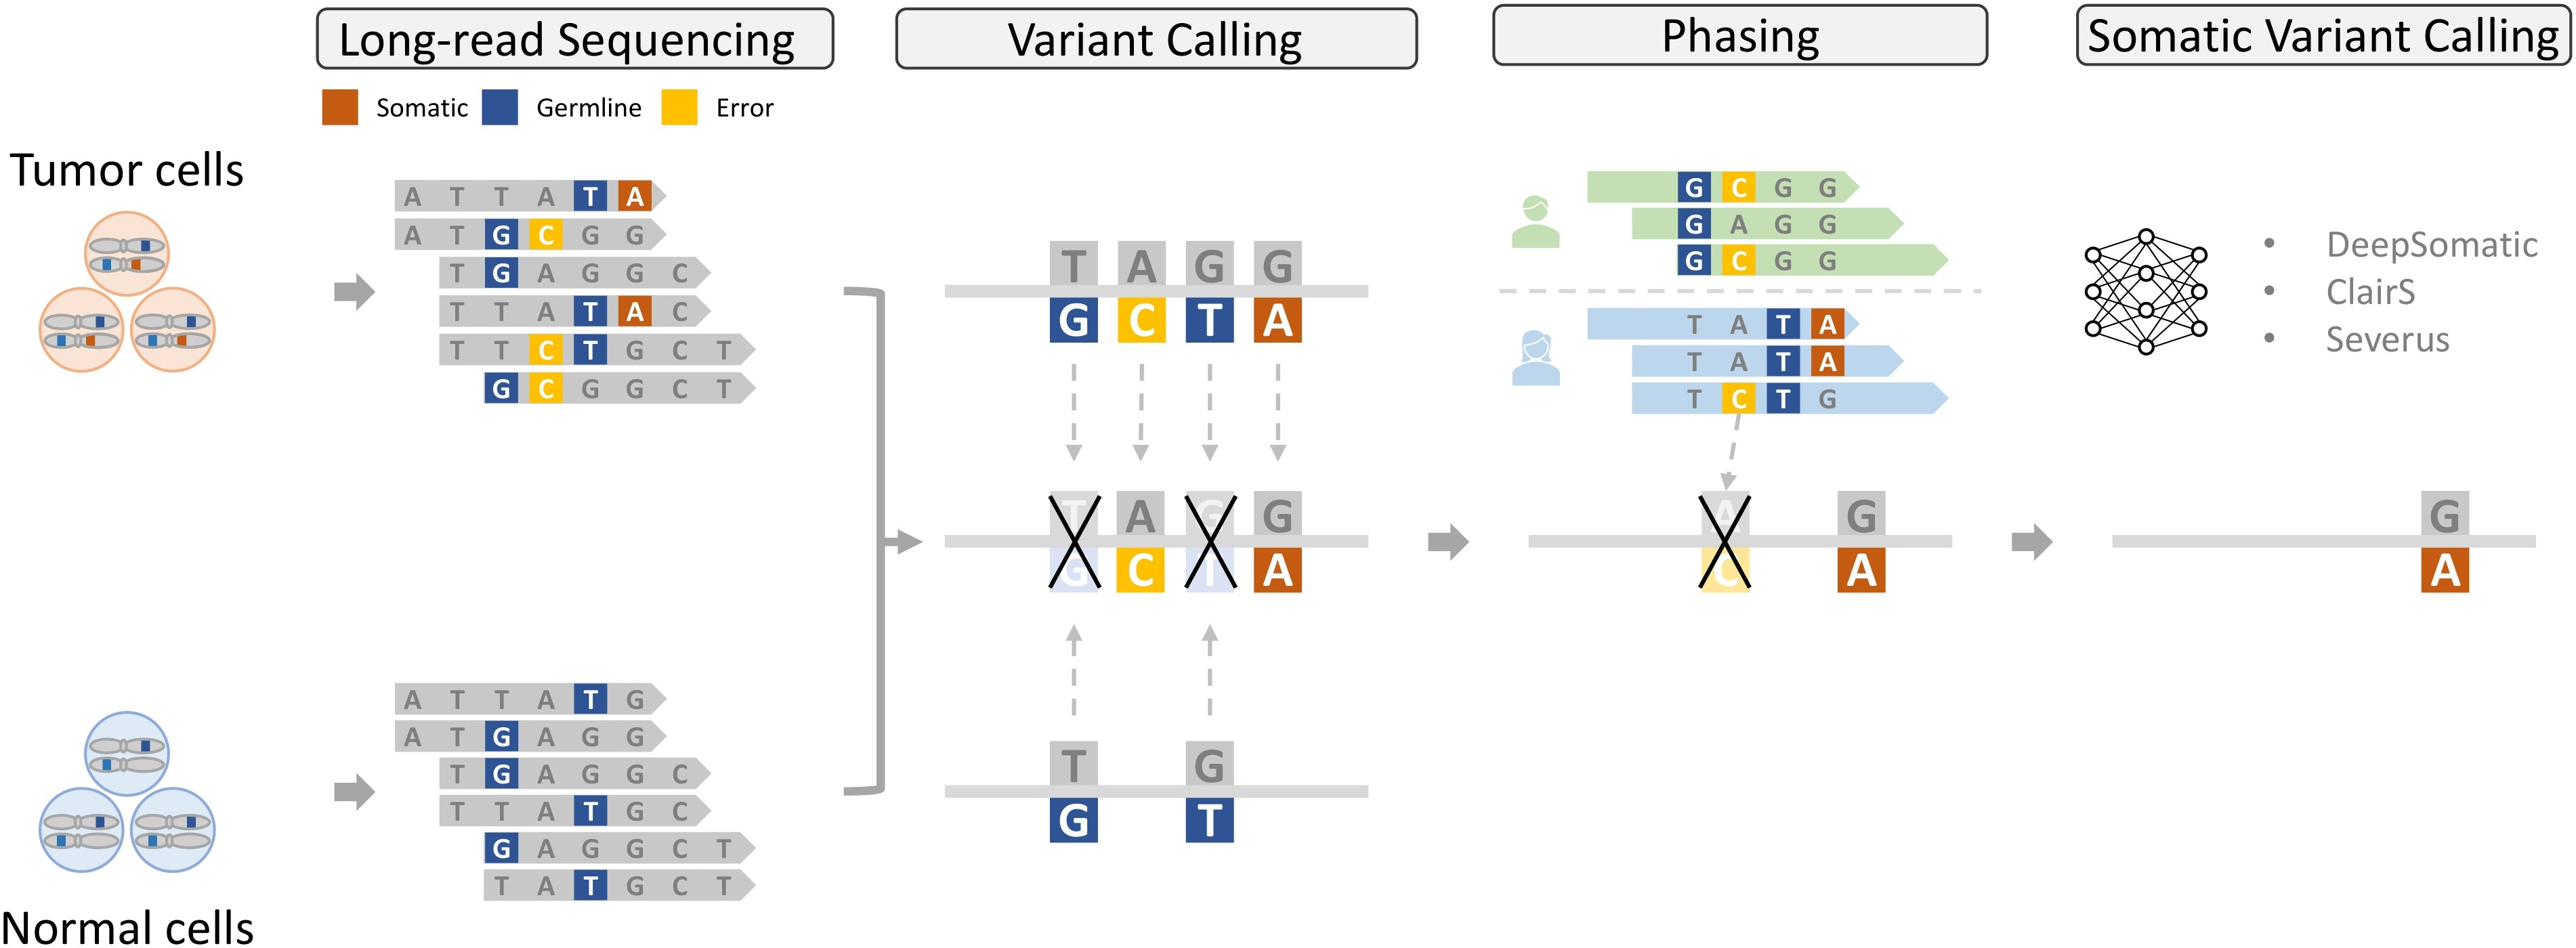
\includegraphics[keepaspectratio,alt={Workflow for somatic variant calling using paired tumor-normal long-read data. After sequencing both samples, variants are called and then phased in the tumor sample. The phasing step (Step 3) segregates reads by haplotype, concentrating the signal of a somatic mutation (orange) onto one haplotype and separating it from the wild-type allele, which improves the signal-to-noise ratio for machine learning-based callers like DeepSomatic or ClairS.}]{page_5_cropped.jpg}}
\caption{Workflow for somatic variant calling using paired tumor-normal long-read data. After sequencing both samples, variants are called and then phased in the tumor sample. The phasing step (Step 3) segregates reads by haplotype, concentrating the signal of a somatic mutation (orange) onto one haplotype and separating it from the wild-type allele, which improves the signal-to-noise ratio for machine learning-based callers like DeepSomatic or ClairS.}\label{fig:int-page-5-cropped-jpg}
\end{figure}

In many clinical and research settings, however, a matched normal sample is unavailable, which necessitates a tumor-only workflow. This scenario presents a significant analytical challenge: differentiating a true, low-frequency somatic mutation from a rare germline variant without a constitutional baseline from the same individual~\cite{sun2018, hiltemann2015, chin2023}. The standard mitigation strategy involves filtering candidate variants against a Panel of Normals (PON), a database of common germline variants and recurrent technical artifacts compiled from a large cohort of healthy individuals~\cite{cibulskis2013}. Although this method effectively eliminates many non-somatic variants, the substantial inter-individual variability means that no database can comprehensively capture all mutations. Consequently, specialized tumor-only callers such as ClairS-TO continue to rely on phasing to enhance the somatic signal, underscoring its indispensable role even in the most challenging data contexts.

Despite these advances, a critical gap persists in the field: the inability of current tools to perform true somatic phasing. Existing methods excel at germline phasing within a tumor sample, meaning that they can separate reads according to the two inherited parental haplotypes. However, they are incapable of reconstructing the novel, complex somatic haplotypes that are the products of a tumor's evolution. Cancer is a dynamic process characterized by clonal evolution, where successive rounds of mutation and selection give rise to a heterogeneous population of subclones, each possessing a unique genetic identity~\cite{nowell1976}. Reconstructing the specific somatic haplotypes of these clones is essential for understanding co-mutation patterns, tracing tumor lineage, and deciphering the cooperative mechanisms that drive malignancy. This represents a frontier in cancer genomics that current methodologies have yet to cross.

The path toward accurate somatic phasing is obstructed by two major biological and computational hurdles inherent to cancer genomes. The first is the prevalence of large-scale structural changes, particularly Loss of Heterozygosity (LOH), where vast regions of a chromosome lose one of the two parental copies~\cite{zheng2005, zhang2021, hwang2021}. Such events disrupt the continuity of heterozygous markers upon which standard algorithms depend, leading to algorithmic failure and the production of fragmented, biologically inaccurate phase blocks. Achieving contiguous, chromosome-scale phasing requires a framework that can explicitly model and navigate these genomic discontinuities. The second challenge is tumor purity; clinical tumor samples are almost invariably a mixture of cancer cells and contaminating normal cells~\cite{yadav2015, zheng2017, rhee2018}. This cellular heterogeneity introduces conflicting haplotype signals into the sequencing data, which confounds phasing algorithms and prevents the reliable determination of the haplotype of somatic origin.

This thesis aims to overcome these fundamental limitations by developing \textbf{LongPhase-TO}, an integrated computational framework for the comprehensive analysis of tumor-only long-read sequencing data. The primary objective is to advance beyond conventional variant calling to achieve true somatic phasing. Through the development of novel algorithms, this method is designed to reconstruct the evolutionary lineage of somatic haplotypes that define a tumor's clonal architecture; to robustly handle chromosome-scale LOH, ensuring contiguous and accurate phasing across complex genomic rearrangements; and to jointly estimate tumor purity, thereby deconvolving the mixed signals from tumor and normal cells to prevent phasing errors. By addressing these challenges within a unified model, this work seeks to provide a more precise and complete reconstruction of the cancer genome, enabling deeper insights into the evolutionary dynamics of tumorigenesis.

\section{Results}\label{results}

This chapter presents the empirical evaluation of the developed methodologies for analyzing tumor-only long-read sequencing data. The results are structured to first establish the superiority of a somatic-aware phasing approach, followed by an in-depth analysis of its application to key downstream tasks, including Loss of Heterozygosity (LOH) detection, somatic variant calling refinement, and tumor purity estimation. The chapter concludes with qualitative visualizations that demonstrate the power of the integrated pipeline in resolving complex genomic events within cancer samples.

\subsection{Superiority of Somatic-Aware Phasing for Tumor-Only Data}\label{superiority-of-somatic-aware-phasing-for-tumor-only-data}

A fundamental prerequisite for analyzing allele-specific events in tumors is the accurate phasing of genetic variants into parental haplotypes. Standard germline phasing tools are designed to handle only heterozygous variants; however, in somatic cell lines, loss of heterozygosity (LOH) frequently eliminates heterozygosity. In this context, LongPhase-TO extends the capability by also incorporating homozygous variants, thereby enabling more comprehensive phasing. To evaluate this approach, the performance of the standard germline phaser LongPhase was compared with the proposed somatic-aware phaser LongPhase-TO. Both tools were tested on eight cancer cell line datasets, using variant calls generated by ClairS-TO in two different modes (ssrs and ss) as input. Performance was assessed based on phasing completeness (Phased Ratio) and contiguity (Block N50) (Figure~\ref{fig:met-page-29-cropped-jpg}).

\begin{figure}
\centering
\pandocbounded{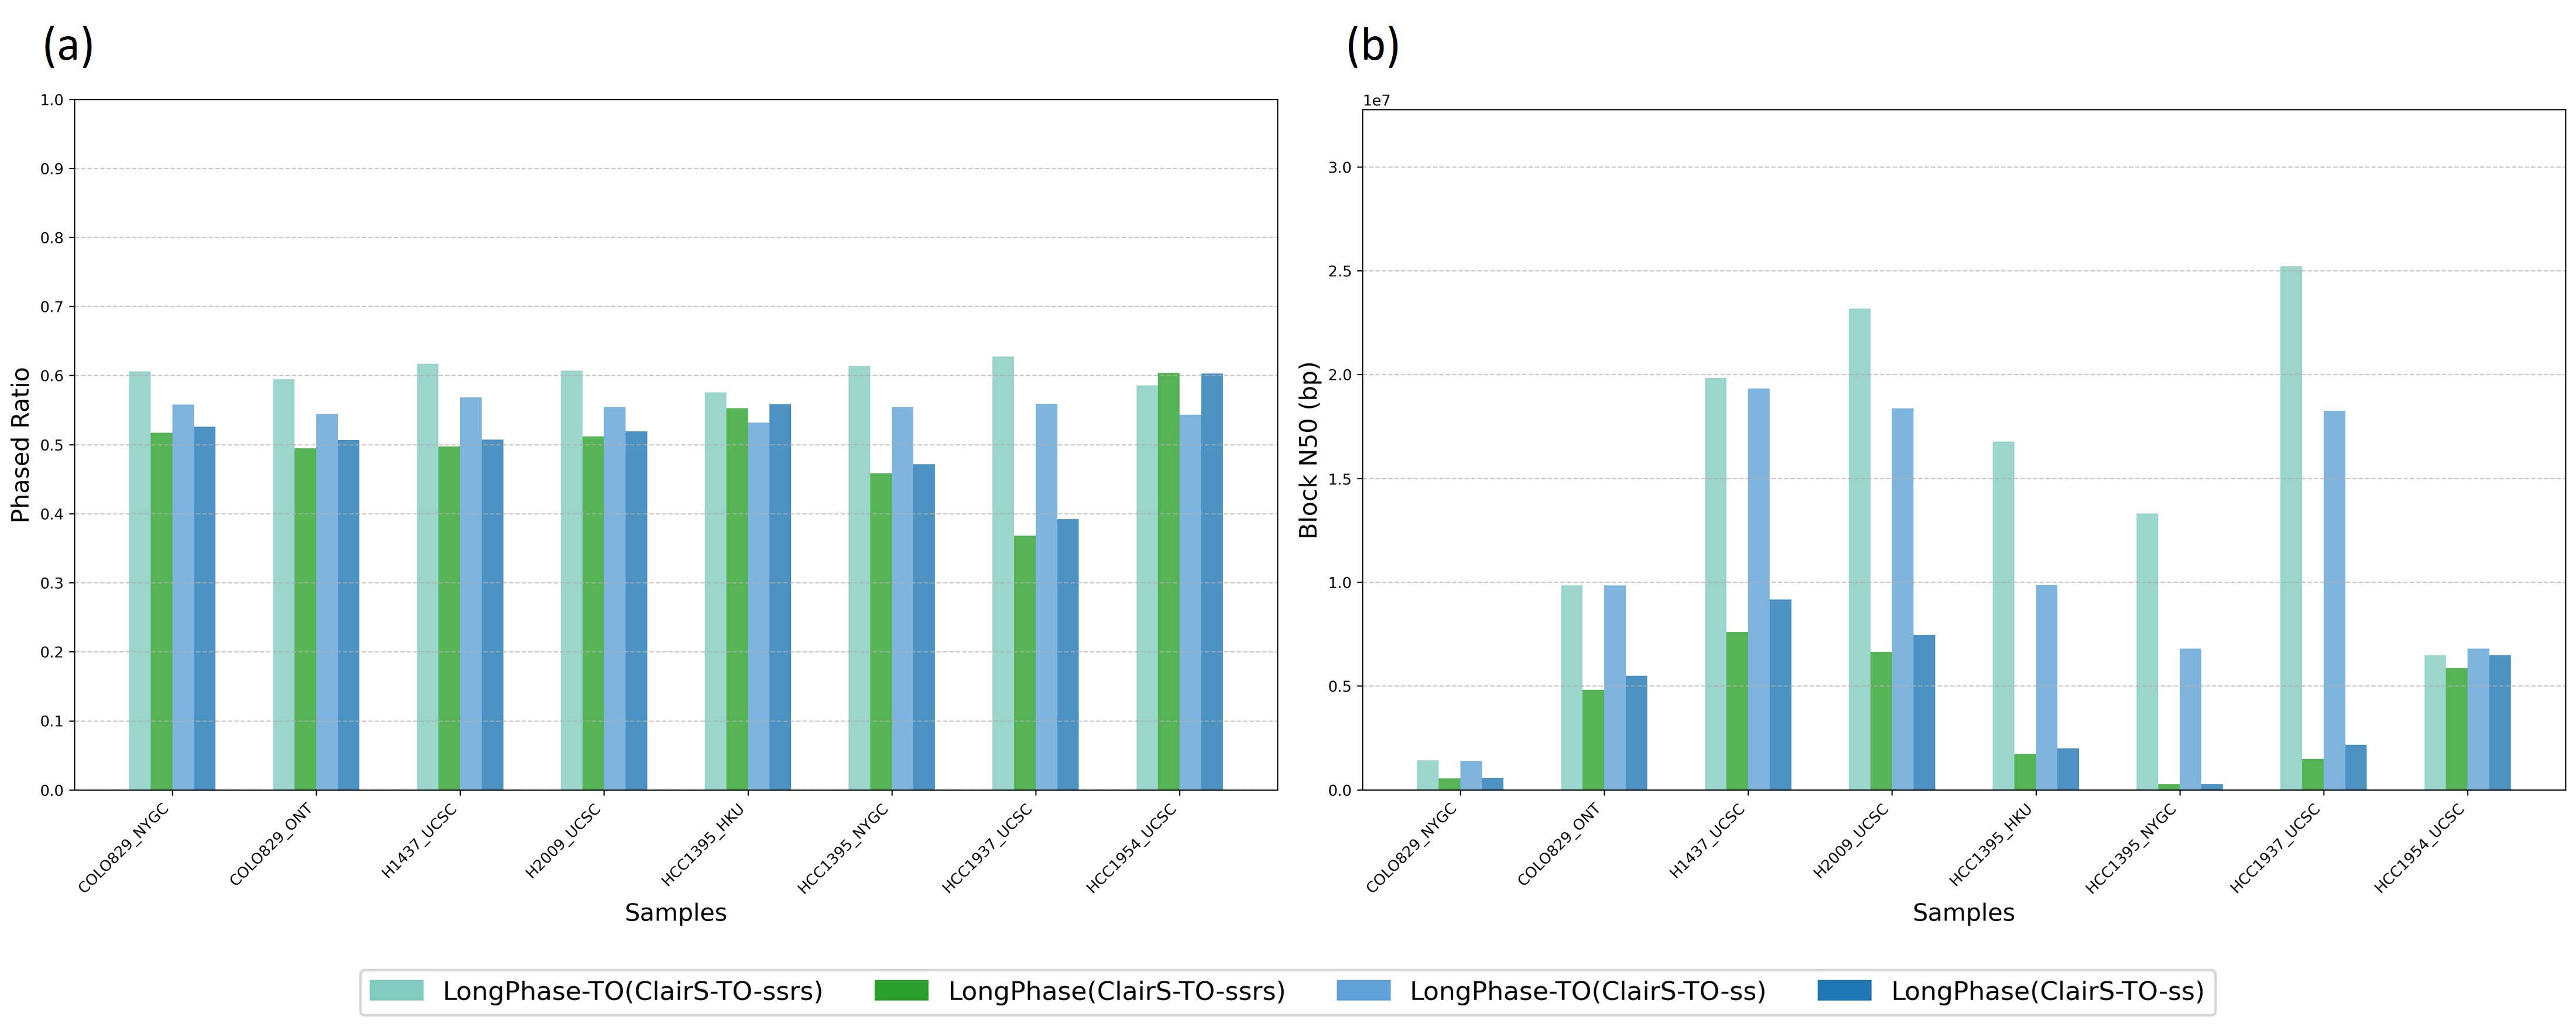
\includegraphics[keepaspectratio]{page_29_cropped.jpg}}
\caption[Comparison of Somatic-aware and Germline Phasers]{Performance comparison of LongPhase-TO (somatic-aware) and LongPhase (germline) across eight cancer cell line datasets. Bars represent four pipelines: LongPhase-TO with ClairS-TO-ssrs calls (teal) and ClairS-TO-ss calls (light blue), and LongPhase with the same two variant sets (green and dark blue). (a) Phased Ratio: LongPhase-TO consistently achieves higher phasing completeness across all samples and input variant sets, typically in the range of 0.55–0.62. (b) Block N50: LongPhase-TO produces substantially longer phase blocks—often spanning several megabases and, in some datasets, reaching 20–25 Mb—whereas LongPhase results in shorter N50 values. These results indicate that incorporating homozygous sites through somatic-aware phasing improves both completeness and contiguity in tumor-only sequencing data.}\label{fig:met-page-29-cropped-jpg}
\end{figure}

The results demonstrate a clear advantage for the somatic-aware LongPhase-TO tool. LongPhase-TO consistently achieved higher Phased Ratios across multiple cancer cell line samples, irrespective of the input variant set. This reflects its ability to account for tumor genome complexities, including variable allele frequencies, the presence of somatic mutations, and the frequent occurrence of homozygous regions caused by LOH.

This advantage is even more pronounced when considering phasing contiguity, a critical metric for the analysis of large-scale genomic events. A second analysis revealed a dramatic difference in Block N50 values. The LongPhase-TO pipelines produced highly contiguous phase blocks, with N50 values frequently ranging between 10 and 25 million base pairs (Mbp). In contrast, the germline LongPhase tool consistently failed to generate long-range phase information, with Block N50 values typically falling below 1 Mbp. This vast improvement in contiguity underscores the necessity of a somatic-aware model for reconstructing long, continuous haplotypes from tumor sequencing data. The ability to generate such long-range phase blocks is essential for accurately identifying structural variations such as LOH. In summary, these findings validate the use of LongPhase-TO as the core phasing engine for all subsequent analyses in this study.

\subsection{Application and Validation of Phasing for LOH Detection}\label{application-and-validation-of-phasing-for-loh-detection}

Having established the superior phasing capabilities of LongPhase-TO, we next evaluated its direct application in detecting Loss of Heterozygosity (LOH), a common and significant event in cancer~\cite{ryland2015, nichols2020}. This evaluation involved two stages: first, optimizing the input for the LOH detection pipeline, and second, validating the final pipeline against a gold-standard orthogonal technology.

\subsubsection{Impact of Input Somatic Variant Calls on LOH Detection}\label{impact-of-input-somatic-variant-calls-on-loh-detection}

To evaluate the feasibility of detecting chromosome-scale loss of heterozygosity (LOH) in tumor cell lines, three distinct variant-calling inputs were analyzed using LongPhase-TO across multiple cancer samples. The results revealed consistent overall trends among datasets, while substantial inter-sample variation was observed (Figure~\ref{fig:met-page-28-cropped-jpg}).

In terms of LOH ratio, the COLO sample exhibited LOH in approximately 30\% of the genome. Comparable patterns were observed in other cell lines, with HCC1395 displaying nearly half of its genome under LOH. Regarding the largest LOH segments, the COLO sample contained a segment of approximately 110 Mb, corresponding to nearly half the length of chromosome 1; other cell lines also harbored similarly large segments.

In contrast, the HCC1954\_UCSC sample showed lower LOH ratios and shorter LOH segments relative to the other cell lines. Overall, these findings demonstrate pronounced variability in LOH across tumor cell lines and underscore the effectiveness of LongPhase-TO in detecting chromosome-scale genomic alterations.

\begin{figure}
\centering
\pandocbounded{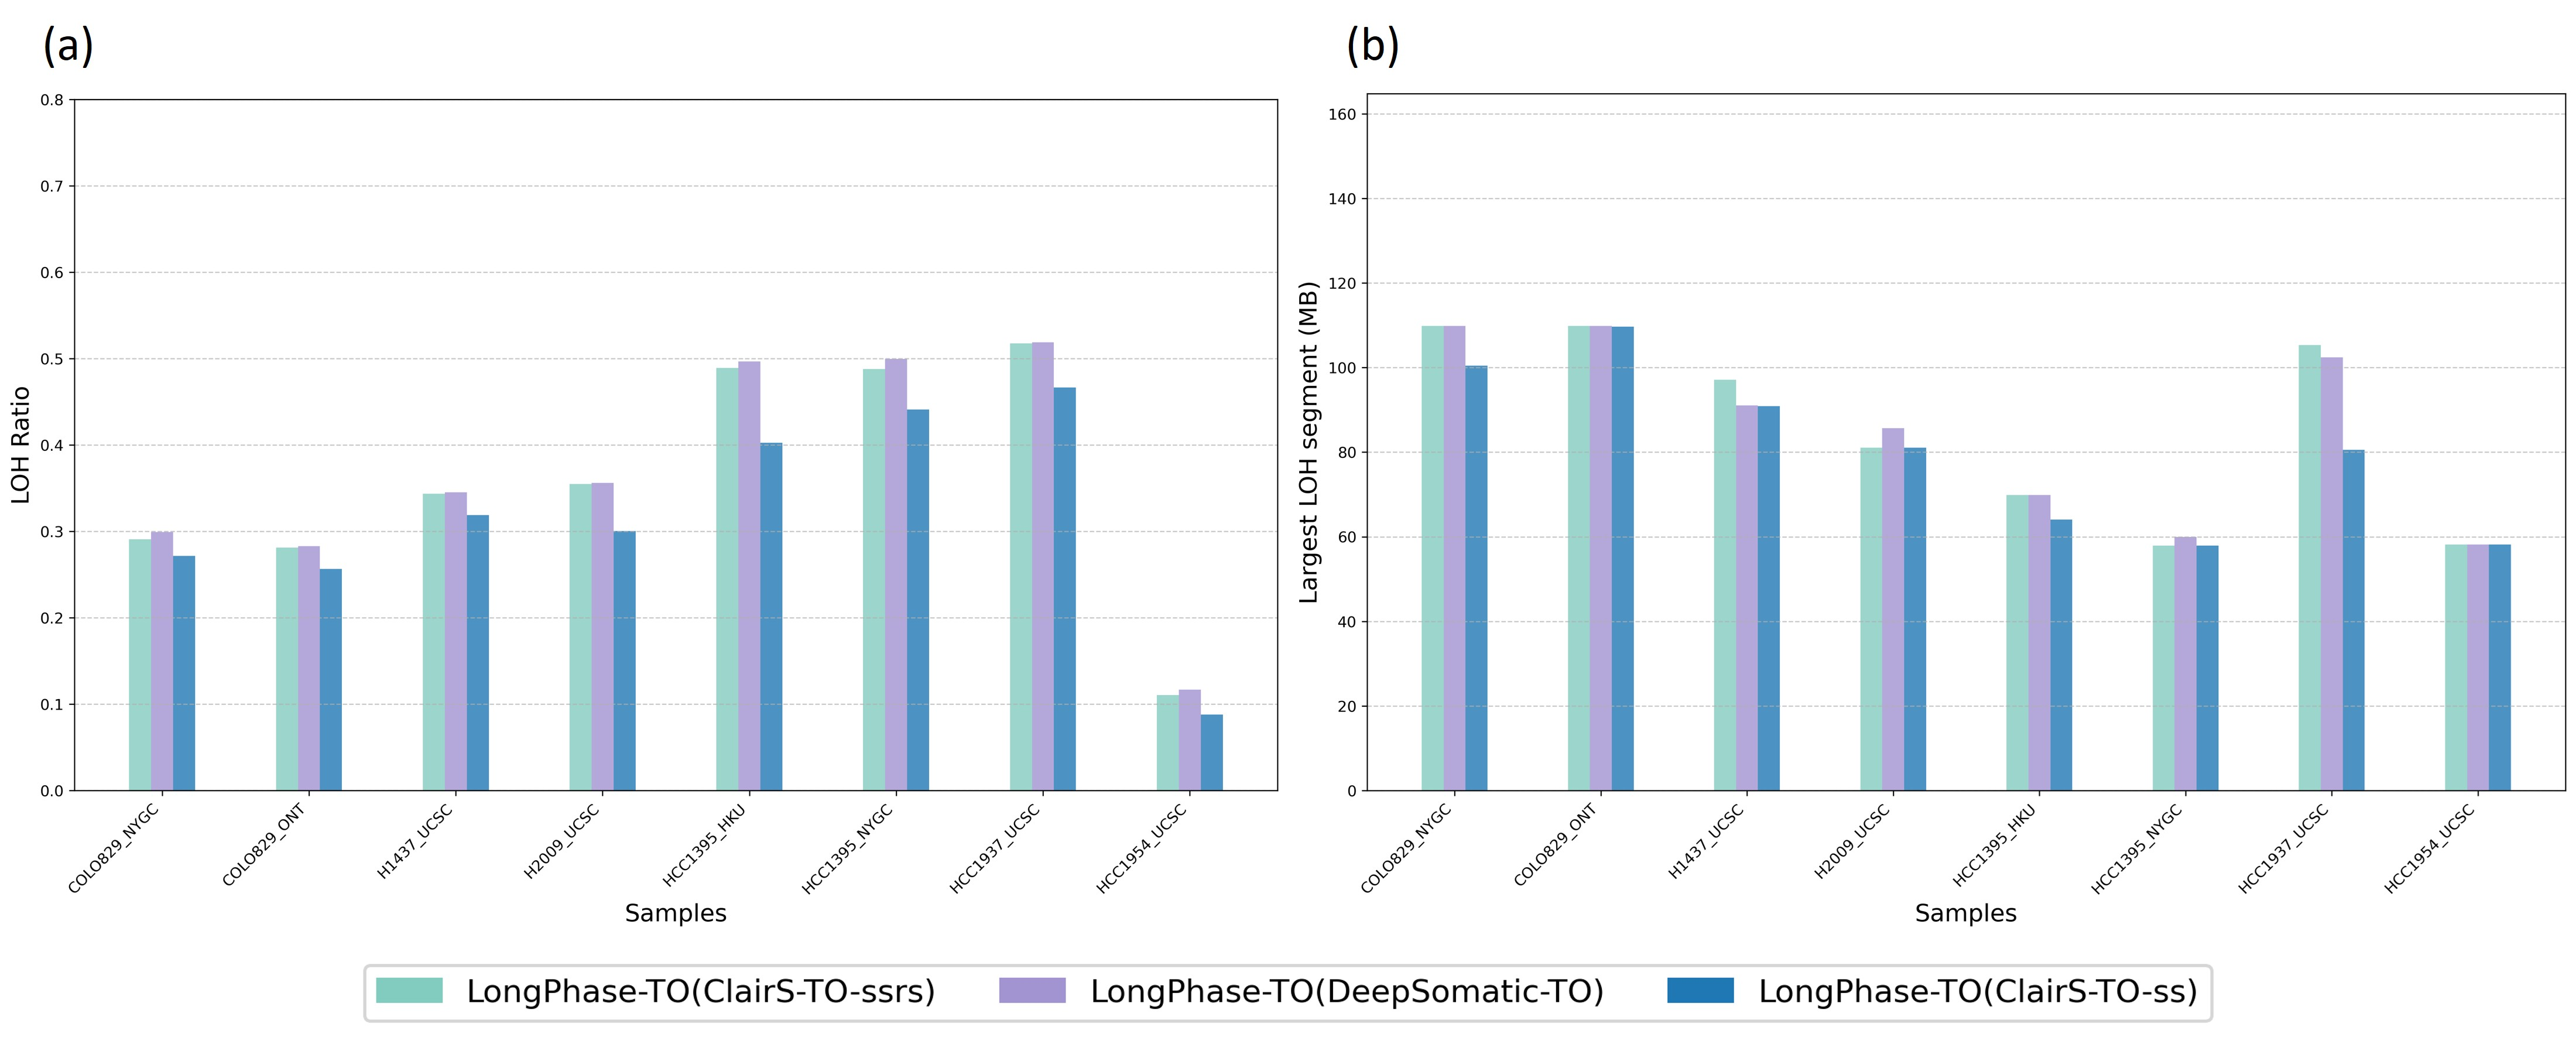
\includegraphics[keepaspectratio]{page_28_cropped.jpg}}
\caption[Comparison of LOH Detection Ratios]{Comparison of LOH ratio across multiple cancer samples using three different LongPhase-TO configurations. Panel (a) shows LOH ratio distributions for each sample, while panel (b) presents the size of the largest LOH segment in megabases. Consistent trends were observed across the different variant-calling inputs, although substantial variation was evident among individual cell lines.}\label{fig:met-page-28-cropped-jpg}
\end{figure}

\subsubsection{Validation Against Microarray-Based LOH Profiles}\label{validation-against-microarray-based-loh-profiles}

To validate the accuracy of our sequencing-based LOH detection method, we performed a head-to-head comparison against results from the Affymetrix CytoScan HD array, a widely used and well-established microarray platform for detecting copy number alterations and LOH~\cite{garciadiez2019, fang2021}. This analysis was conducted on the HCC1395\_HKU cancer cell line, with LOH calls from our LongPhase-TO pipeline compared against the CytoScan HD reference across the entire genome (Figure~\ref{fig:met-page-30-cropped-jpg}).

\begin{figure}
\centering
\pandocbounded{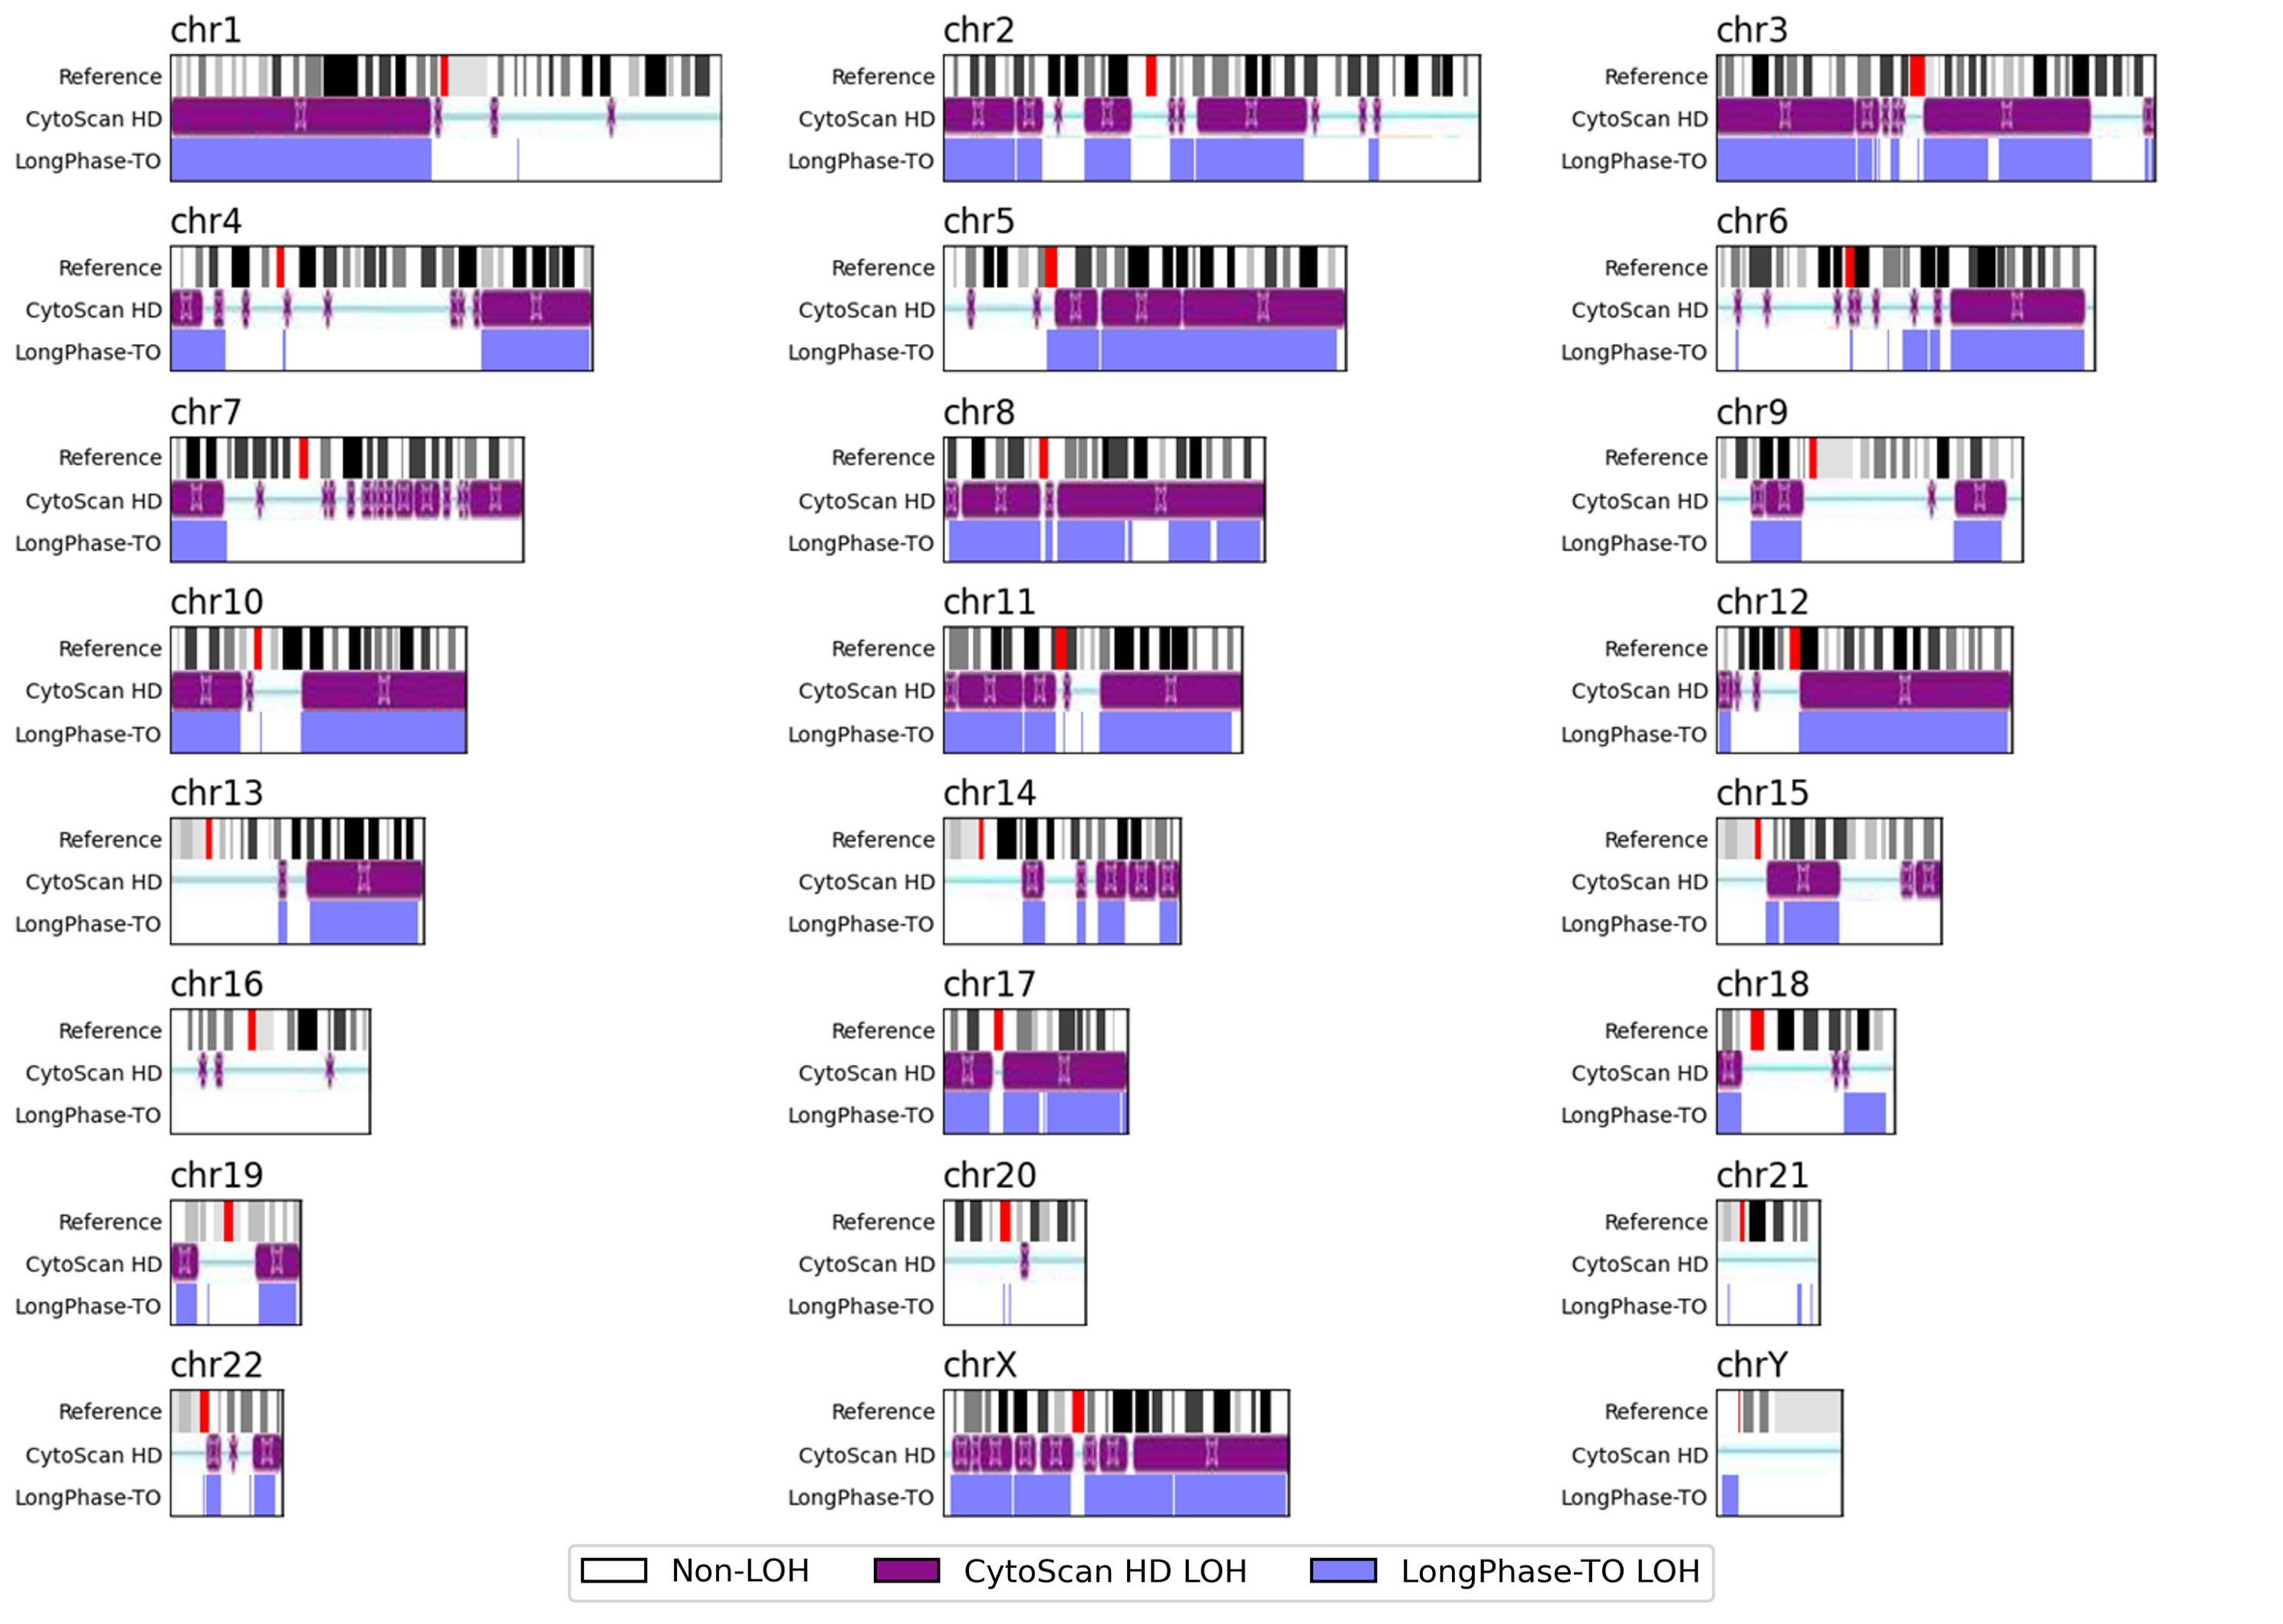
\includegraphics[keepaspectratio]{page_30_cropped.jpg}}
\caption[Genome-wide validation of LOH detection]{Genome-wide comparison of LOH profiles between the sequencing-based LongPhase-TO pipeline (blue) and the Affymetrix CytoScan HD array (purple) in the HCC1395\_HKU cancer cell line. Across all chromosomes, a high degree of concordance is observed between the two platforms, indicating that LongPhase-TO reliably recapitulates microarray-based LOH detection at chromosome scale.}\label{fig:met-page-30-cropped-jpg}
\end{figure}

A genome-wide visualization, presenting each chromosome from 1 to 22, \(X\), and \(Y\), reveals a remarkably high level of concordance between the two methods. For each chromosome, the LOH regions detected by the LongPhase-TO pipeline (represented by blue bars in the corresponding figure) show near-perfect overlap with the LOH regions detected by the CytoScan HD array (purple bars). This strong agreement is evident across numerous chromosomes, including large-scale events on chromosomes 1, 3, 5, 8, 10, 11, 12, 17, and \(X\). The long, contiguous LOH blocks identified by LongPhase-TO are a direct manifestation of its superior long-range phasing capability. This visual validation provides compelling evidence that the LongPhase-TO-based methodology accurately identifies known, large-scale LOH events, confirming its efficacy and reliability as a tool for LOH analysis from tumor-only long-read sequencing data.

\subsection{Refining Somatic Variant Calls with Phasing Information}\label{refining-somatic-variant-calls-with-phasing-information}

Beyond LOH detection, haplotype information can be leveraged to refine the accuracy of upstream somatic variant calling~\cite{zhou2024}. We investigated the impact of integrating LongPhase-TO as a post-processing filter for somatic single nucleotide variant (SNV) calls. This was assessed by comparing the performance of base callers with and without the LongPhase-TO refinement step, using models trained on both real and simulated data.

\subsubsection{Performance on Models Trained with Real Data}\label{performance-on-models-trained-with-real-data}

We first evaluated the impact of LongPhase-TO on two state-of-the-art somatic callers, ClairS-TO-ssrs and DeepSomatic-TO, using models trained on real sequencing data. The performance of four pipelines—the two base callers alone and the two in combination with LongPhase-TO—was benchmarked across eight cancer cell line datasets at varying levels of simulated tumor purity (20\% to 100\%). Performance was measured using the F1-score, precision, and recall (Figure~\ref{fig:met-page-31-cropped-jpg}).

The results, presented in a comprehensive grid of performance plots, show that applying LongPhase-TO as a filter has a distinct and significant effect on each base caller. For ClairS-TO-ssrs, the addition of LongPhase-TO consistently improves both precision and the overall F1-score across nearly all datasets and purity levels. This indicates that LongPhase-TO acts as an effective filter, removing false positives from the ClairS-TO-ssrs call set and thereby increasing its overall accuracy. In the case of DeepSomatic-TO, the baseline caller exhibited very high recall but insufficient precision. Incorporating LongPhase-TO markedly enhanced its precision, thereby improving the reliability of the resulting call set. Together, these observations demonstrate that LongPhase-TO can systematically refine outputs from distinct somatic callers, albeit with caller-specific trade-offs.

For the HCC1937 dataset, precision exhibited a marked improvement of approximately 20\% across tumor purity levels ranging from 0.2 to 0.8, while recall showed modest reductions that varied with purity. Nevertheless, the overall F1-score consistently increased, reflecting the net gain in accuracy. Similar patterns were observed across the other cancer cell line datasets: precision was substantially improved in nearly all cases, whereas recall showed varying degrees of reduction. Importantly, when integrated into the F1-score, these trade-offs consistently resulted in an overall enhancement of performance.

As expected, the performance of all tested pipelines generally improved with increasing tumor purity, as the higher proportion of tumor DNA makes somatic variants more readily distinguishable from the germline background. These results validate LongPhase-TO as a powerful refinement tool that can enhance the accuracy of somatic variant calling.


\begin{figure}
\centering
\pandocbounded{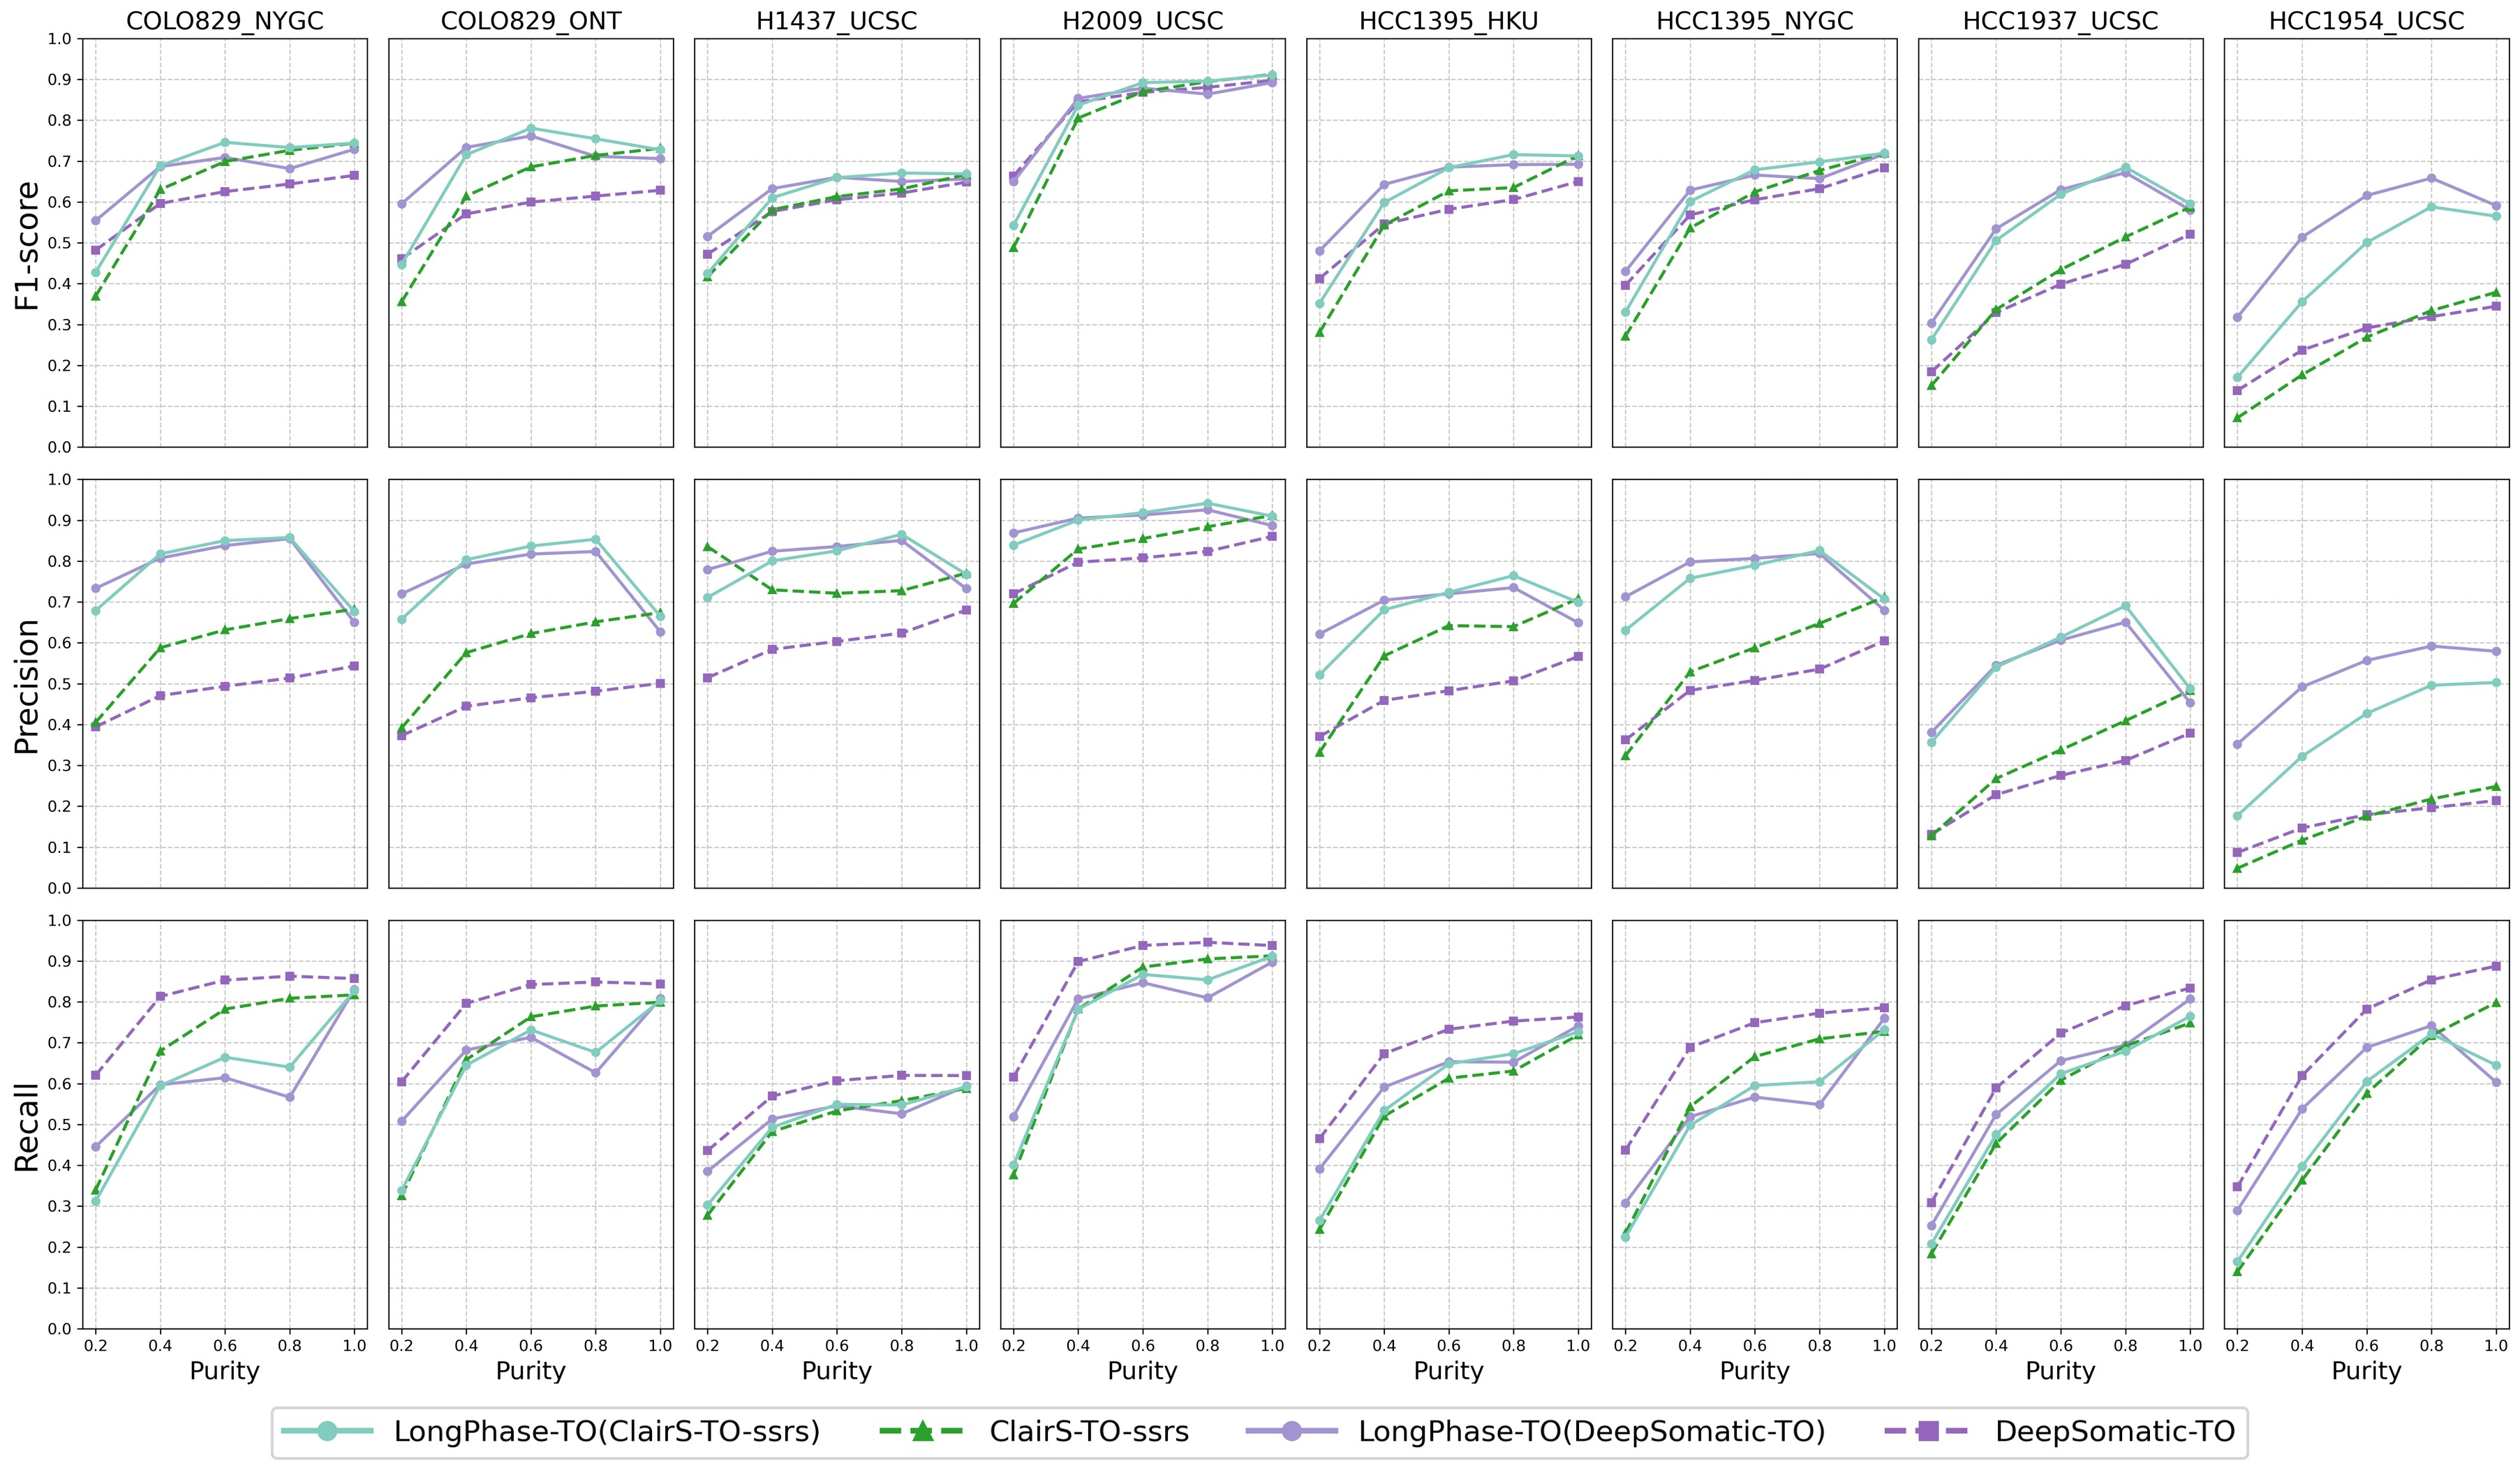
\includegraphics[keepaspectratio]{page_31_cropped.jpg}}
\caption[Somatic variant calling performance with Real Data]{Performance comparison of ClairS-TO-ssrs and DeepSomatic-TO, with and without LongPhase-TO, across eight cancer cell line datasets under varying tumor purities (20\%–100\%). Incorporation of LongPhase-TO consistently increased precision and F1-score, with modest reductions in recall. Overall, LongPhase-TO improved the accuracy of somatic variant detection, particularly at intermediate tumor purity levels.}\label{fig:met-page-31-cropped-jpg}
\end{figure}
% ~\cite{weber2020, kuo2023, cosentino2019}.

\subsubsection{Characterization of the Precision-Recall Trade-off using Simulation-Trained Models}\label{characterization-of-the-precision-recall-trade-off-using-simulation-trained-models}

To further investigate the filtering characteristics of LongPhase-TO, we conducted a benchmark using a variant caller (ClairS-TO-ss) trained on simulated data. This controlled experiment enables a clear characterization of the precision–recall dynamics when LongPhase-TO is applied as a post-processing step. The performance of ClairS-TO-ss with and without LongPhase-TO was evaluated across the same eight datasets and purity levels.

The results unequivocally demonstrate that LongPhase-TO functions as a precision-enhancing filter. Across all eight datasets, the combined LongPhase-TO(ClairS-TO-ss) pipeline consistently achieved significantly higher precision compared to ClairS-TO-ss alone. This improvement, however, was consistently accompanied by a decrease in recall, confirming that the filtering process removes some true positive variants alongside false positives. Importantly, the relative impact of LongPhase-TO exhibited greater consistency at lower tumor purity levels, where gains in precision were more stable across datasets. The net effect on the F1-score, which balances precision and recall, was context-dependent. In datasets where the baseline precision of ClairS-TO-ss was lower, the gain in precision from LongPhase-TO outweighed the loss in recall, resulting in a higher F1-score. In other cases, the trade-off was less favorable. Collectively, these findings confirm the role of LongPhase-TO as a conservative but effective filter for somatic variant calls, offering a robust mechanism to increase confidence in the final call set, particularly under conditions of reduced tumor purity.

\begin{figure}
\centering
\pandocbounded{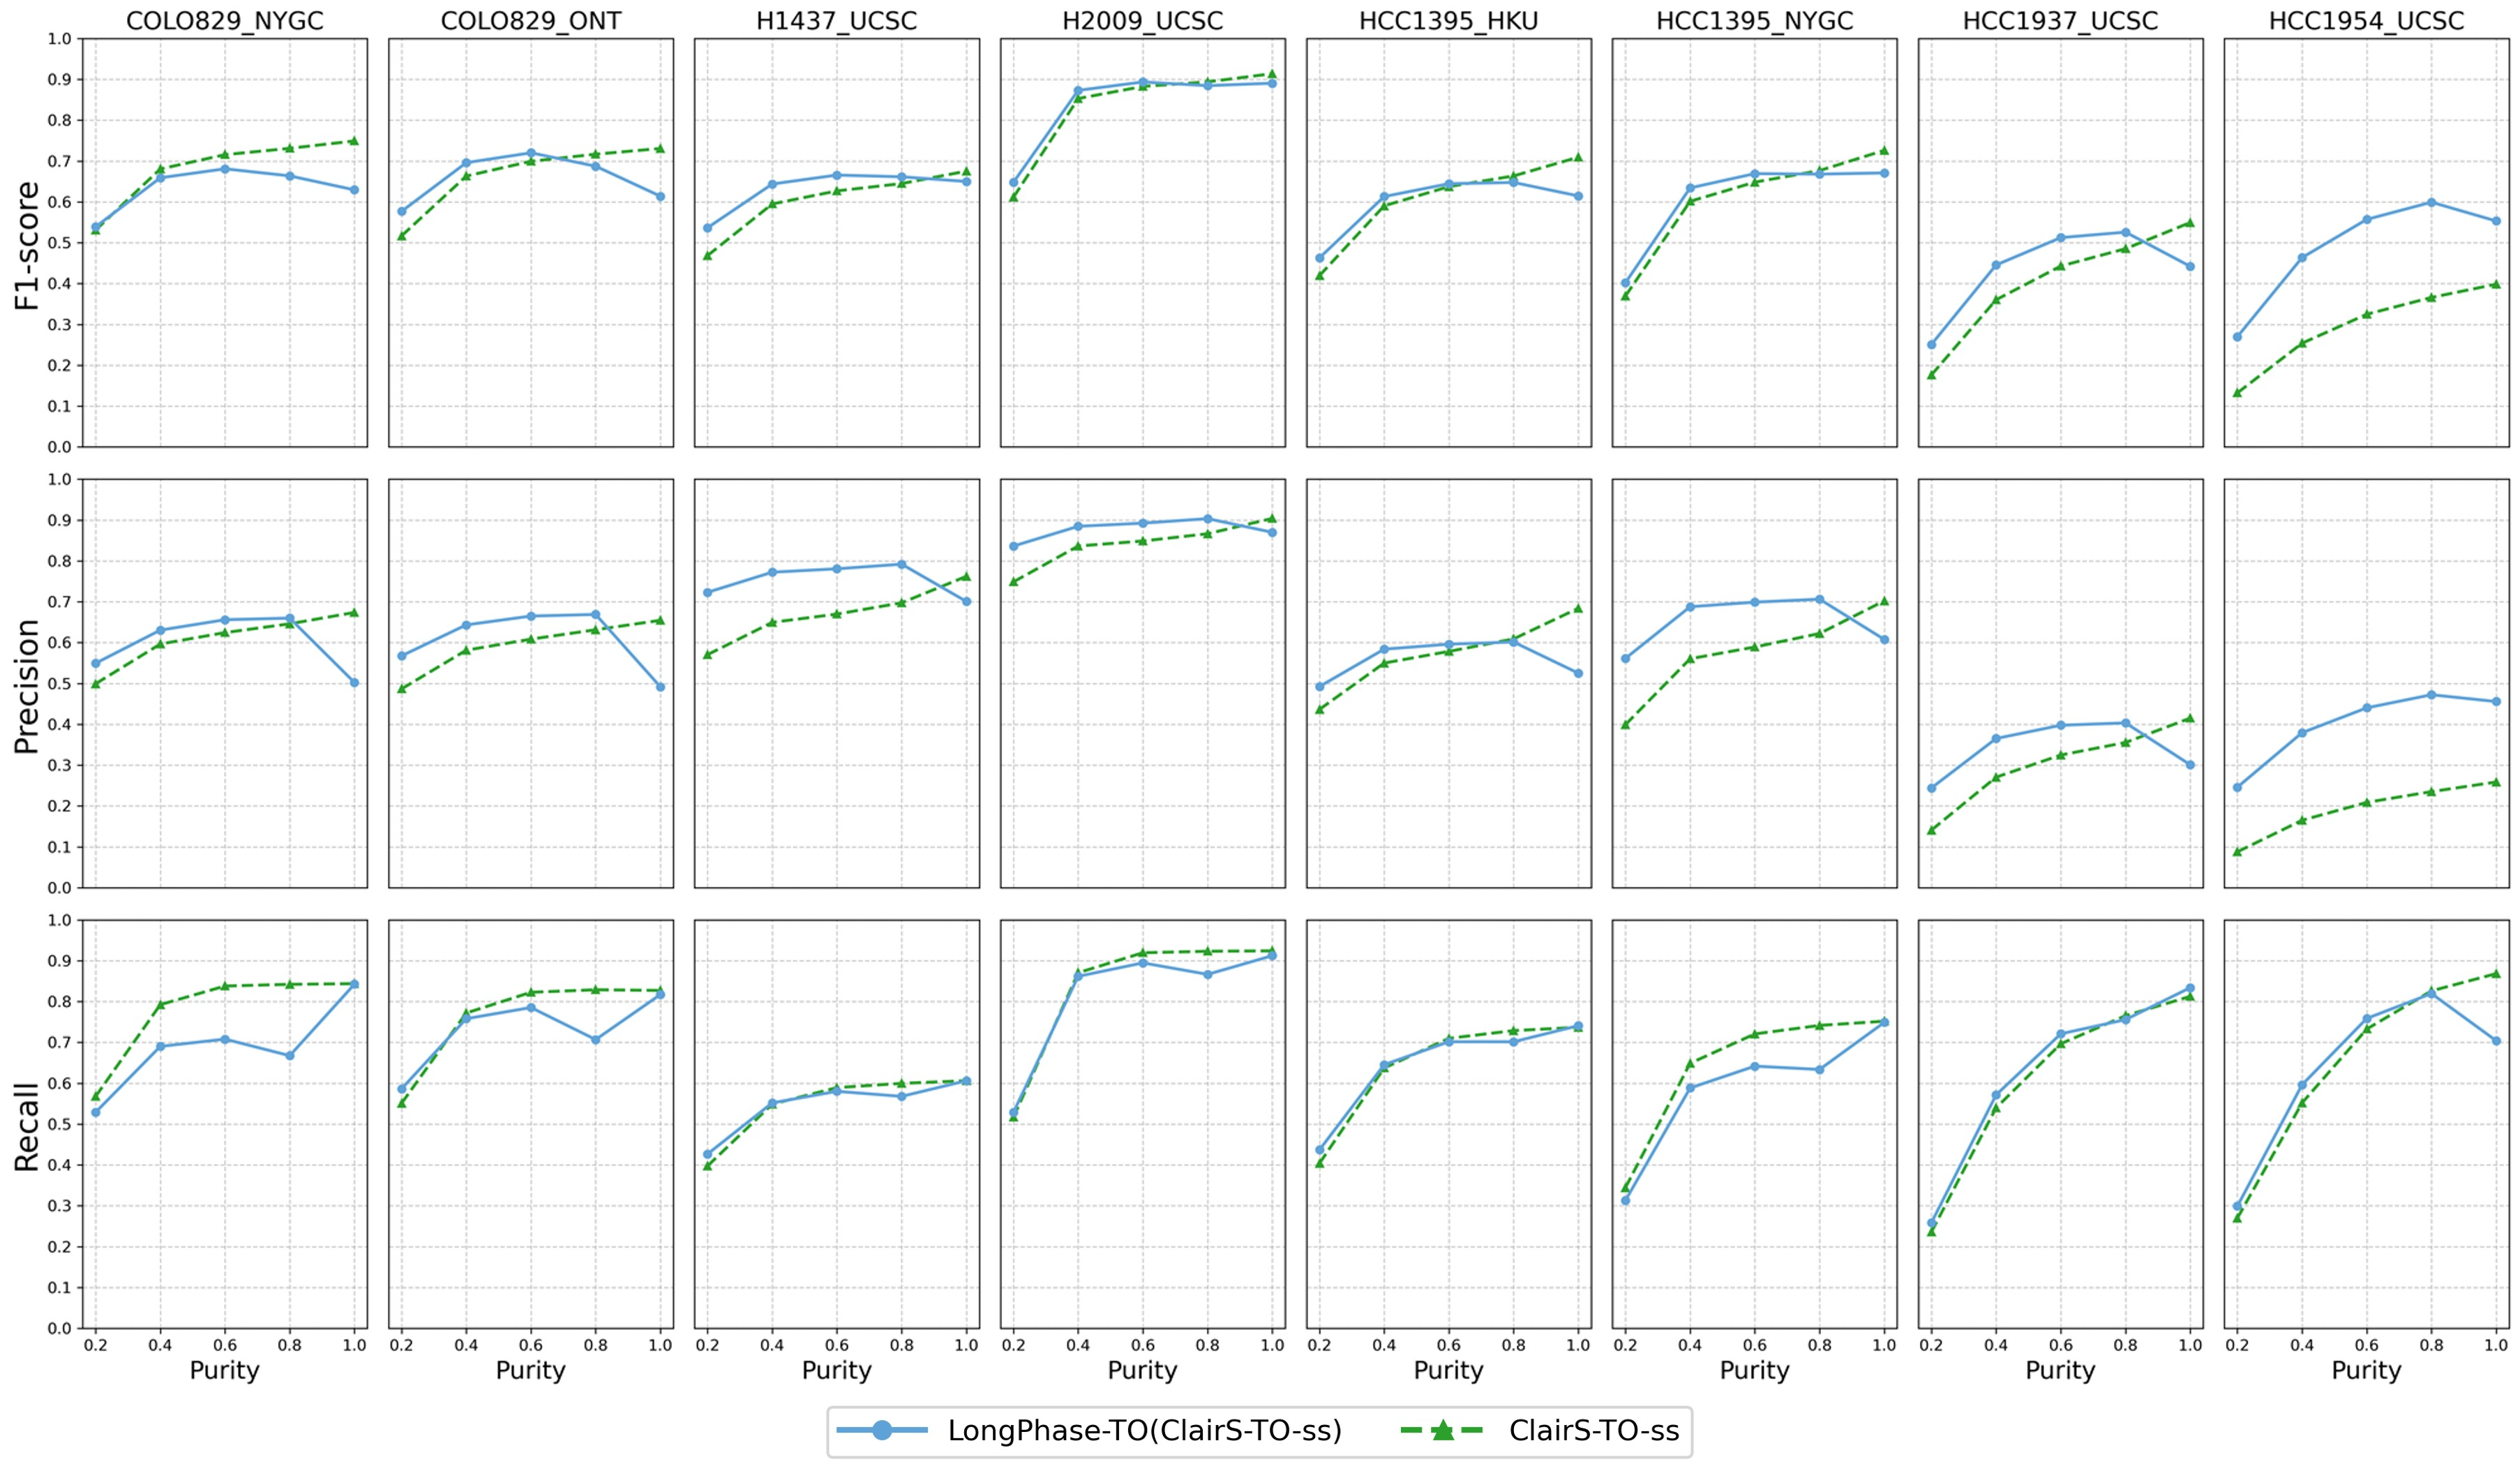
\includegraphics[keepaspectratio]{page_32_cropped.jpg}}
\caption[Somatic variant calling performance with Simulation-Trained]{Somatic variant calling performance of ClairS-TO-ss with and without LongPhase-TO across eight cancer cell line datasets at tumor purities from 20\% to 100\%. LongPhase-TO generally improved precision, while recall was reduced to varying degrees.}
\label{fig:met-page-32-cropped-jpg}
\end{figure}

\subsection{Accurate Tumor Purity Estimation from Tumor-Only Long-Read Data}\label{accurate-tumor-purity-estimation-from-tumor-only-long-read-data}

An accurate estimate of tumor purity is a critical parameter for interpreting cancer genomics data~\cite{koo2021, zhang2015}. We assessed the capability of our LongPhase-TO-based pipelines to predict tumor purity directly from tumor-only long-read sequencing data. The purity estimates from three LongPhase-TO pipeline variants were compared against those from ASCAT, a widely used tool that requires matched tumor–normal data, using simulated purity as the ground truth (Figure~\ref{fig:met-page-33-cropped-jpg}).

\begin{figure}
\centering
\pandocbounded{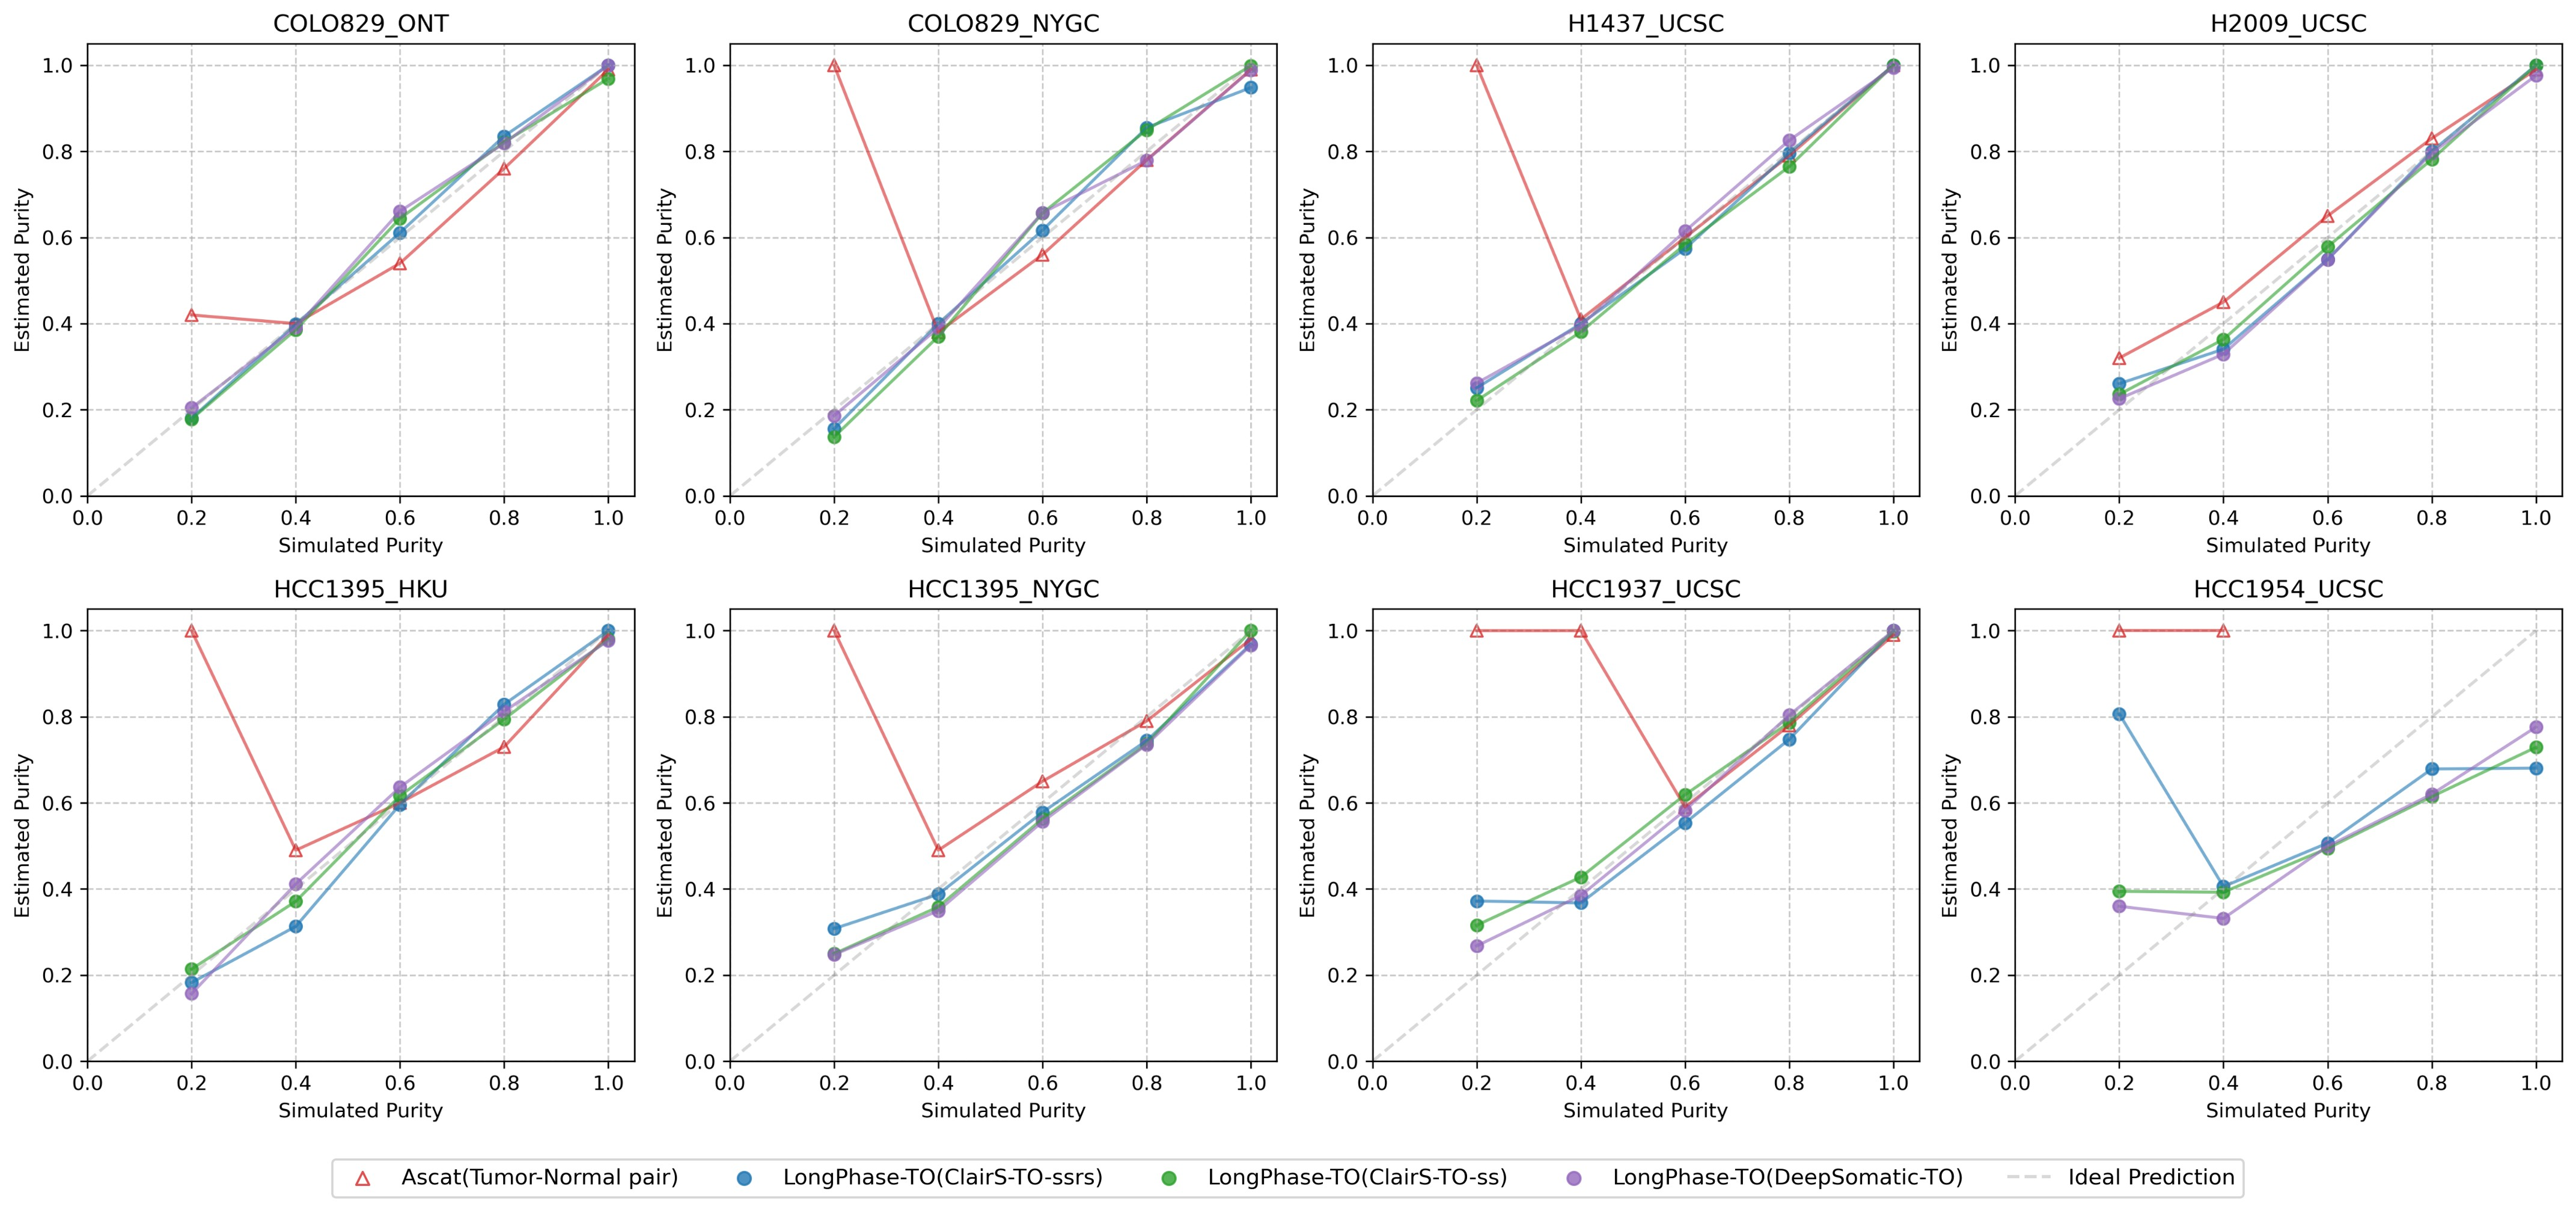
\includegraphics[keepaspectratio]{page_33_cropped.jpg}}
\caption[Performance of tumor purity estimation pipelines]{Estimated tumor purity from three LongPhase-TO variants (LongPhase-TO(ClairS-TO-ssrs), LongPhase-TO(ClairS-TO-ss), and LongPhase-TO(DeepSomatic-TO)) and from ASCAT (tumor–normal paired analysis) was compared with simulated ground truth across eight cancer cell line datasets. Scatter plots display estimated purity (y-axis) against simulated purity (x-axis), with the diagonal line indicating the ideal prediction ($y=x$). LongPhase-TO pipelines showed high concordance with ground truth across purity levels (20–100\%), with minor deviations at 20\%. ASCAT exhibited greater variability, particularly at low purities.}
\label{fig:met-page-33-cropped-jpg}
\end{figure}

The evaluation, conducted across eight cancer cell line datasets, demonstrates the strong performance of the LongPhase-TO-based methods. In a series of scatter plots comparing estimated purity against simulated purity, the predictions from all three LongPhase-TO pipelines closely tracked the ideal prediction line ($y=x$) across the full range of purity levels (20\% to 100\%). This high accuracy was largely consistent across datasets and appeared independent of the specific upstream variant caller used (ClairS-TO-ssrs, ClairS-TO-ss, or DeepSomatic-TO), suggesting the robustness of the purity estimation algorithm within LongPhase-TO itself. Minor deviations from the ideal prediction line were observed at the lowest simulated purity (20\%), reflecting the inherent challenges of analysis in low-purity samples, though overall performance remained favorable compared to alternative approaches.

In contrast, the ASCAT method exhibited reduced stability at low purity levels, with frequent deviations from the true values and occasional overestimation toward 100\% purity. These findings indicate that the LongPhase-TO framework provides a generally accurate and reliable approach for tumor purity estimation from tumor-only long-read data, offering potential advantages over existing methods that require matched normal samples.

\subsection{Qualitative Demonstration of Haplotype-Resolved Variant Analysis}\label{qualitative-demonstration-of-haplotype-resolved-variant-analysis}

To complement the quantitative benchmarks, we present qualitative evidence from genome browser visualizations that showcase the unique analytical power of our integrated pipeline. These examples illustrate the ability to resolve the haplotype context of individual somatic mutations and complex structural events.

\subsubsection{Visualizing Haplotype-Resolved Somatic Variants}\label{visualizing-haplotype-resolved-somatic-variants}

A key capability of our methodology is haplotagging, which refers to the assignment of a somatic variant to its parental chromosome of origin. A visualization from a cancer sample clearly demonstrates this process. In the displayed genomic region, long sequencing reads are successfully partitioned into two parental haplotypes (HP1 and HP2). A specific somatic variant is observed exclusively on a subset of reads belonging to Haplotype 2. These reads are further isolated into a distinct sub-haplotype track (HP2-1). This visualization provides unambiguous evidence that the somatic mutation occurred on the chromosome corresponding to Haplotype 2. Furthermore, its presence on only a subset of HP2 reads suggests the identification of a tumor subclone, highlighting the method's potential to resolve intra-tumor heterogeneity (Figure~\ref{fig:met-page-34-cropped-jpg}).

\begin{figure}
\centering
\pandocbounded{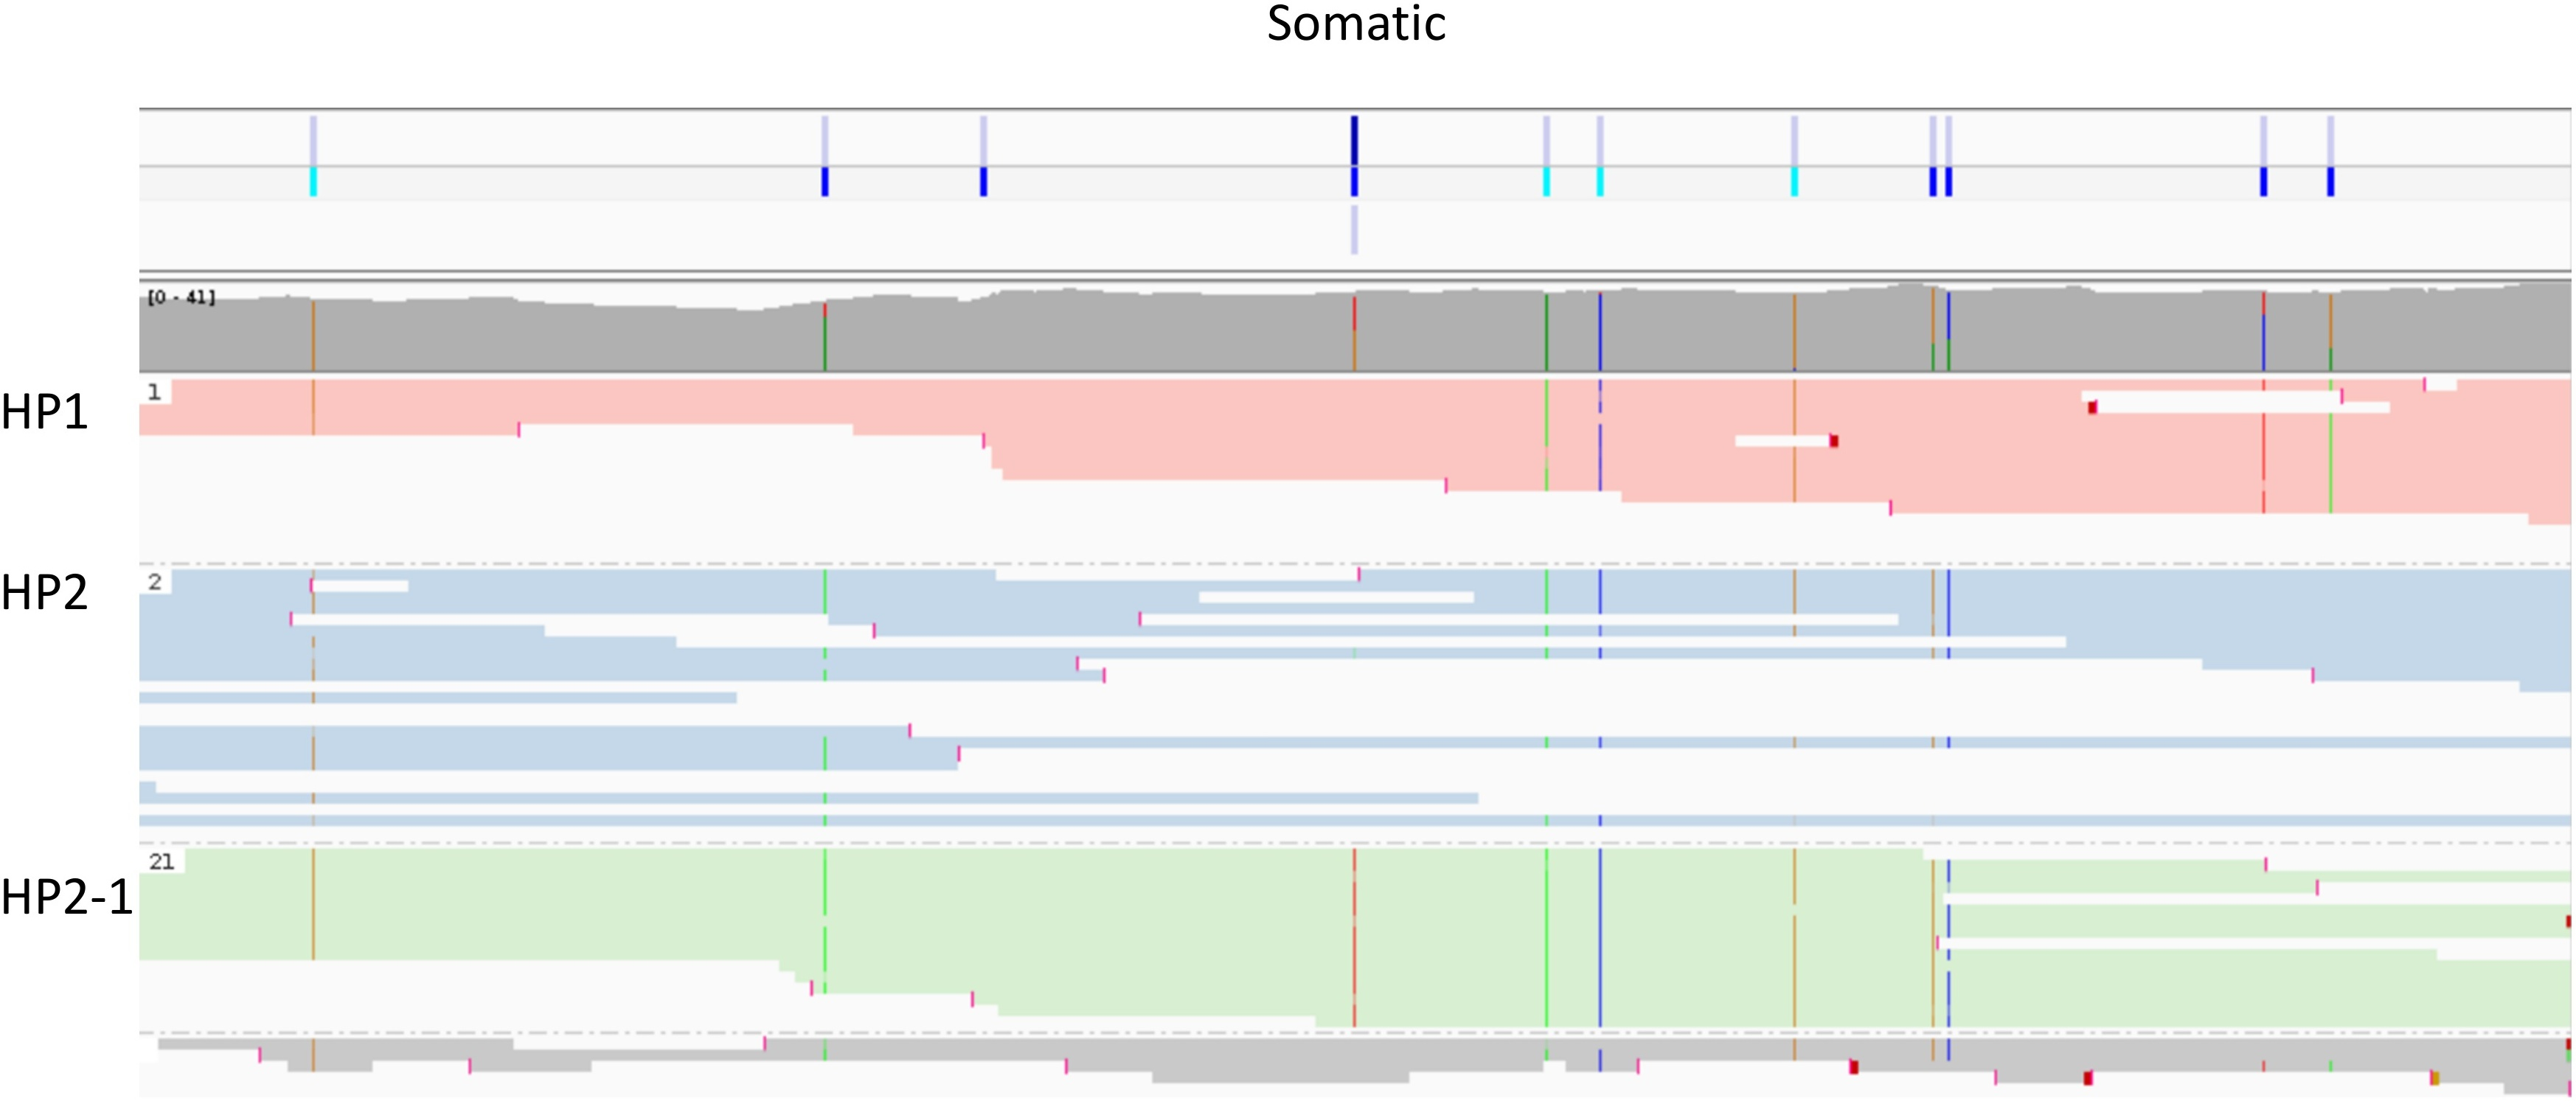
\includegraphics[keepaspectratio]{page_34_cropped.jpg}}
\caption[Visualization of haplotype-resolved somatic variants from long-read sequencing.]{Visualization of haplotype-resolved somatic variants from long-read sequencing. Genome browser snapshot illustrating the haplotype assignment (haplotagging) of a somatic variant. Long sequencing reads are partitioned into two parental haplotypes (HP1 and HP2). The somatic variant is detected exclusively on a subset of reads belonging to Haplotype 2, which are further separated into a sub-haplotype track (HP2-1). This provides direct evidence that the mutation originated from the chromosome corresponding to Haplotype 2. Moreover, its presence only on a fraction of HP2 reads indicates the detection of a tumor subclone, highlighting the capability of the method to resolve intra-tumor heterogeneity.}
\label{fig:met-page-34-cropped-jpg}
\end{figure}

\subsubsection{Integrated Analysis of Co-occurring Somatic Alterations}\label{integrated-analysis-of-co-occurring-somatic-alterations}

Cancer genomes are often characterized by the co-occurrence of multiple types of alterations~\cite{sanchezvega2018, saiki2021}. A second, more complex visualization demonstrates the pipeline's power to dissect such scenarios by simultaneously detecting and phasing a large-scale LOH event and a discrete somatic point mutation. In the displayed genome browser view (Figure~\ref{fig:met-page-35-cropped-jpg}), a large region on the left is clearly marked by a complete absence of sequencing reads assigned to Haplotype 1 (HP1), providing a definitive signature of LOH for that parental allele. To the right of this LOH region, the genome is heterozygous. Within this region, a specific somatic point variant is identified and precisely haplotagged. The variant is found exclusively on reads belonging to a sub-clonal population (HP2-1) of the retained Haplotype 2 (HP2).

\begin{figure}
\centering
\pandocbounded{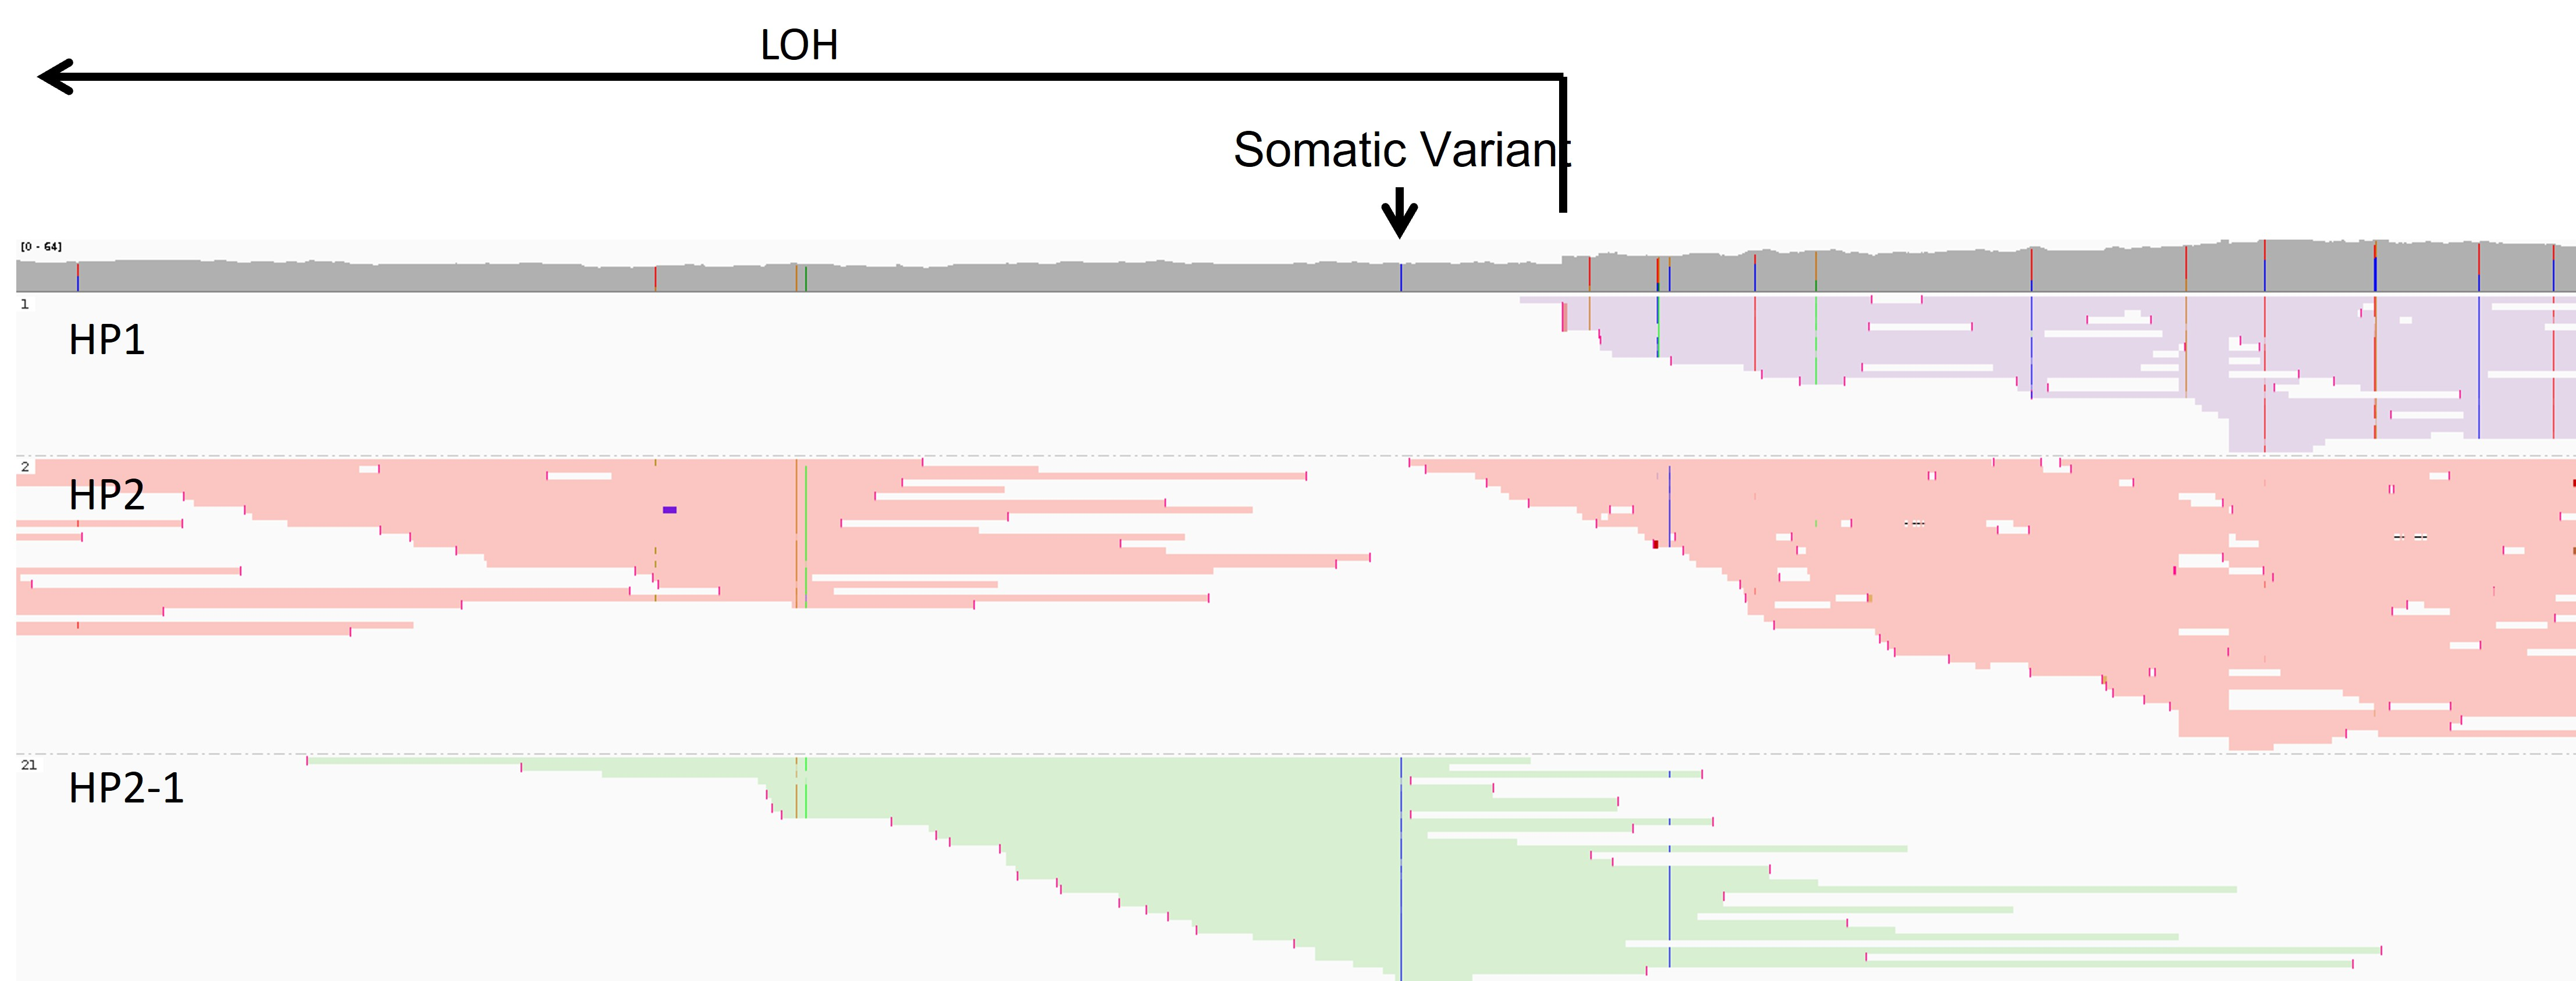
\includegraphics[keepaspectratio]{page_35_cropped.jpg}}
\caption[Integrated visualization of LOH and haplotype-resolved somatic variant]{Integrated visualization of LOH and haplotype-resolved somatic variant.Genome browser snapshot showing the simultaneous detection and phasing of a large-scale loss of heterozygosity (LOH) event and a somatic point mutation. The left genomic region is characterized by the complete absence of sequencing reads from Haplotype 1 (HP1), indicating LOH on this parental allele. To the right, the genome remains heterozygous. Within this region, a somatic point mutation is identified and haplotagged, appearing exclusively on a sub-clonal population (HP2-1) of the retained Haplotype 2 (HP2). This visualization reconstructs a complex mutational history, where LOH resulted in the loss of HP1 and a subsequent somatic mutation occurred on HP2 within a tumor subclone. Such integrative phasing provides critical insights into tumor evolution and the haplotype-specific architecture of somatic alterations.}
\label{fig:met-page-35-cropped-jpg}
\end{figure}

This powerful example illustrates the capacity of the pipeline to reconstruct a complex mutational history: an LOH event resulted in the loss of the HP1 chromosome segment, and a subsequent somatic mutation arose on the remaining HP2 chromosome within a specific subclone. This ability to resolve different classes of somatic events and place them in their correct haplotype context is critical for a deeper understanding of tumor evolution and genetic architecture.


\section{Conclusions}\label{conclusions}

This thesis has addressed the growing need for specialized bioinformatics tools capable of leveraging the unique advantages of long-read sequencing for cancer genomics, particularly in clinical and research settings where only a tumor sample is available. The central contribution of this work is the development and validation of LongPhase-TO, a novel tumor-only analysis pipeline designed to provide a comprehensive, haplotype-resolved view of the somatic landscape. By integrating advanced phasing algorithms with graph-based modeling, this research demonstrates a new paradigm for extracting multi-layered genomic information from a single tumor specimen, thereby overcoming significant limitations of conventional methods.

The key findings of this study underscore the multifaceted capabilities of LongPhase-TO. First, the pipeline achieves accurate somatic phasing, enabling the assignment of somatic mutations to their specific parental chromosome of origin. This capability remains robust even in complex genomic regions, including those undergoing Loss of Heterozygosity (LOH), providing unprecedented resolution into the allelic context of carcinogenesis. Second, LongPhase-TO facilitates the reliable detection of large, chromosome-scale LOH events, with performance comparable to established array-based standards while avoiding the fragmentation issues that can plague other sequencing-based approaches. Third, by leveraging this phasing information, the pipeline significantly enhances the precision of somatic variant calling, a benefit that is particularly pronounced in challenging cases characterized by low tumor purity. Finally, LongPhase-TO introduces a method for accurately estimating tumor purity directly from the sequencing data by analyzing signals of haplotype imbalance and LOH, thereby obviating the need for a matched normal sample and streamlining the analytical workflow.

The implications of this research are significant for both basic cancer biology and clinical oncology. For fundamental research, a haplotype-resolved analysis of the tumor genome offers deeper insights into the mechanisms of tumor evolution, including the specific allelic context of driver mutations and the clonal dynamics of LOH events. From a clinical perspective, the ability to perform robust, comprehensive genomic analysis from a tumor-only sample enhances the utility of long-read sequencing in diagnostic and prognostic settings where obtaining a matched normal sample is impractical or impossible. By delivering reliable LOH detection, improved variant calling, and accurate purity estimation within a single, integrated pipeline, LongPhase-TO is established as a cost-effective and broadly applicable tool for precision medicine.

While this work establishes a powerful new methodology, several avenues for future research can extend its capabilities and applications. Promising directions include the validation of LongPhase-TO across a broader spectrum of cancer types and a larger cohort of patient samples to further assess its generalizability and performance. The pipeline can also be extended to characterize other classes of complex structural variants, such as balanced translocations and chromothripsis, which are increasingly recognized for their role in cancer. Furthermore, integrating LongPhase-TO with other omics data, such as transcriptomics or epigenomics, could provide a more holistic understanding of how genetic and epigenetic alterations cooperate in a haplotype-specific manner to drive tumorigenesis. Such advancements will continue to build upon the foundation laid by this thesis, further unlocking the potential of long-read sequencing to transform our understanding and treatment of cancer.

\section{Methods}\label{methods}

\subsection{Introduction and Overall Objective}\label{introduction-and-overall-objective}

The primary objective of this research is the development and application of LongPhase-TO, a comprehensive bioinformatics pipeline designed for the analysis of tumor-only samples using long-read sequencing data (Figure~\ref{fig:met-page-10-cropped-jpg}). The absence of a matched normal sample in many clinical and research settings poses significant analytical challenges, including the confident identification of somatic mutations and the characterization of tumor-specific genomic aberrations. LongPhase-TO is engineered to overcome these challenges by integrating multiple, haplotype-aware analyses into a single, cohesive workflow.

\begin{figure}  
\centering
\pandocbounded{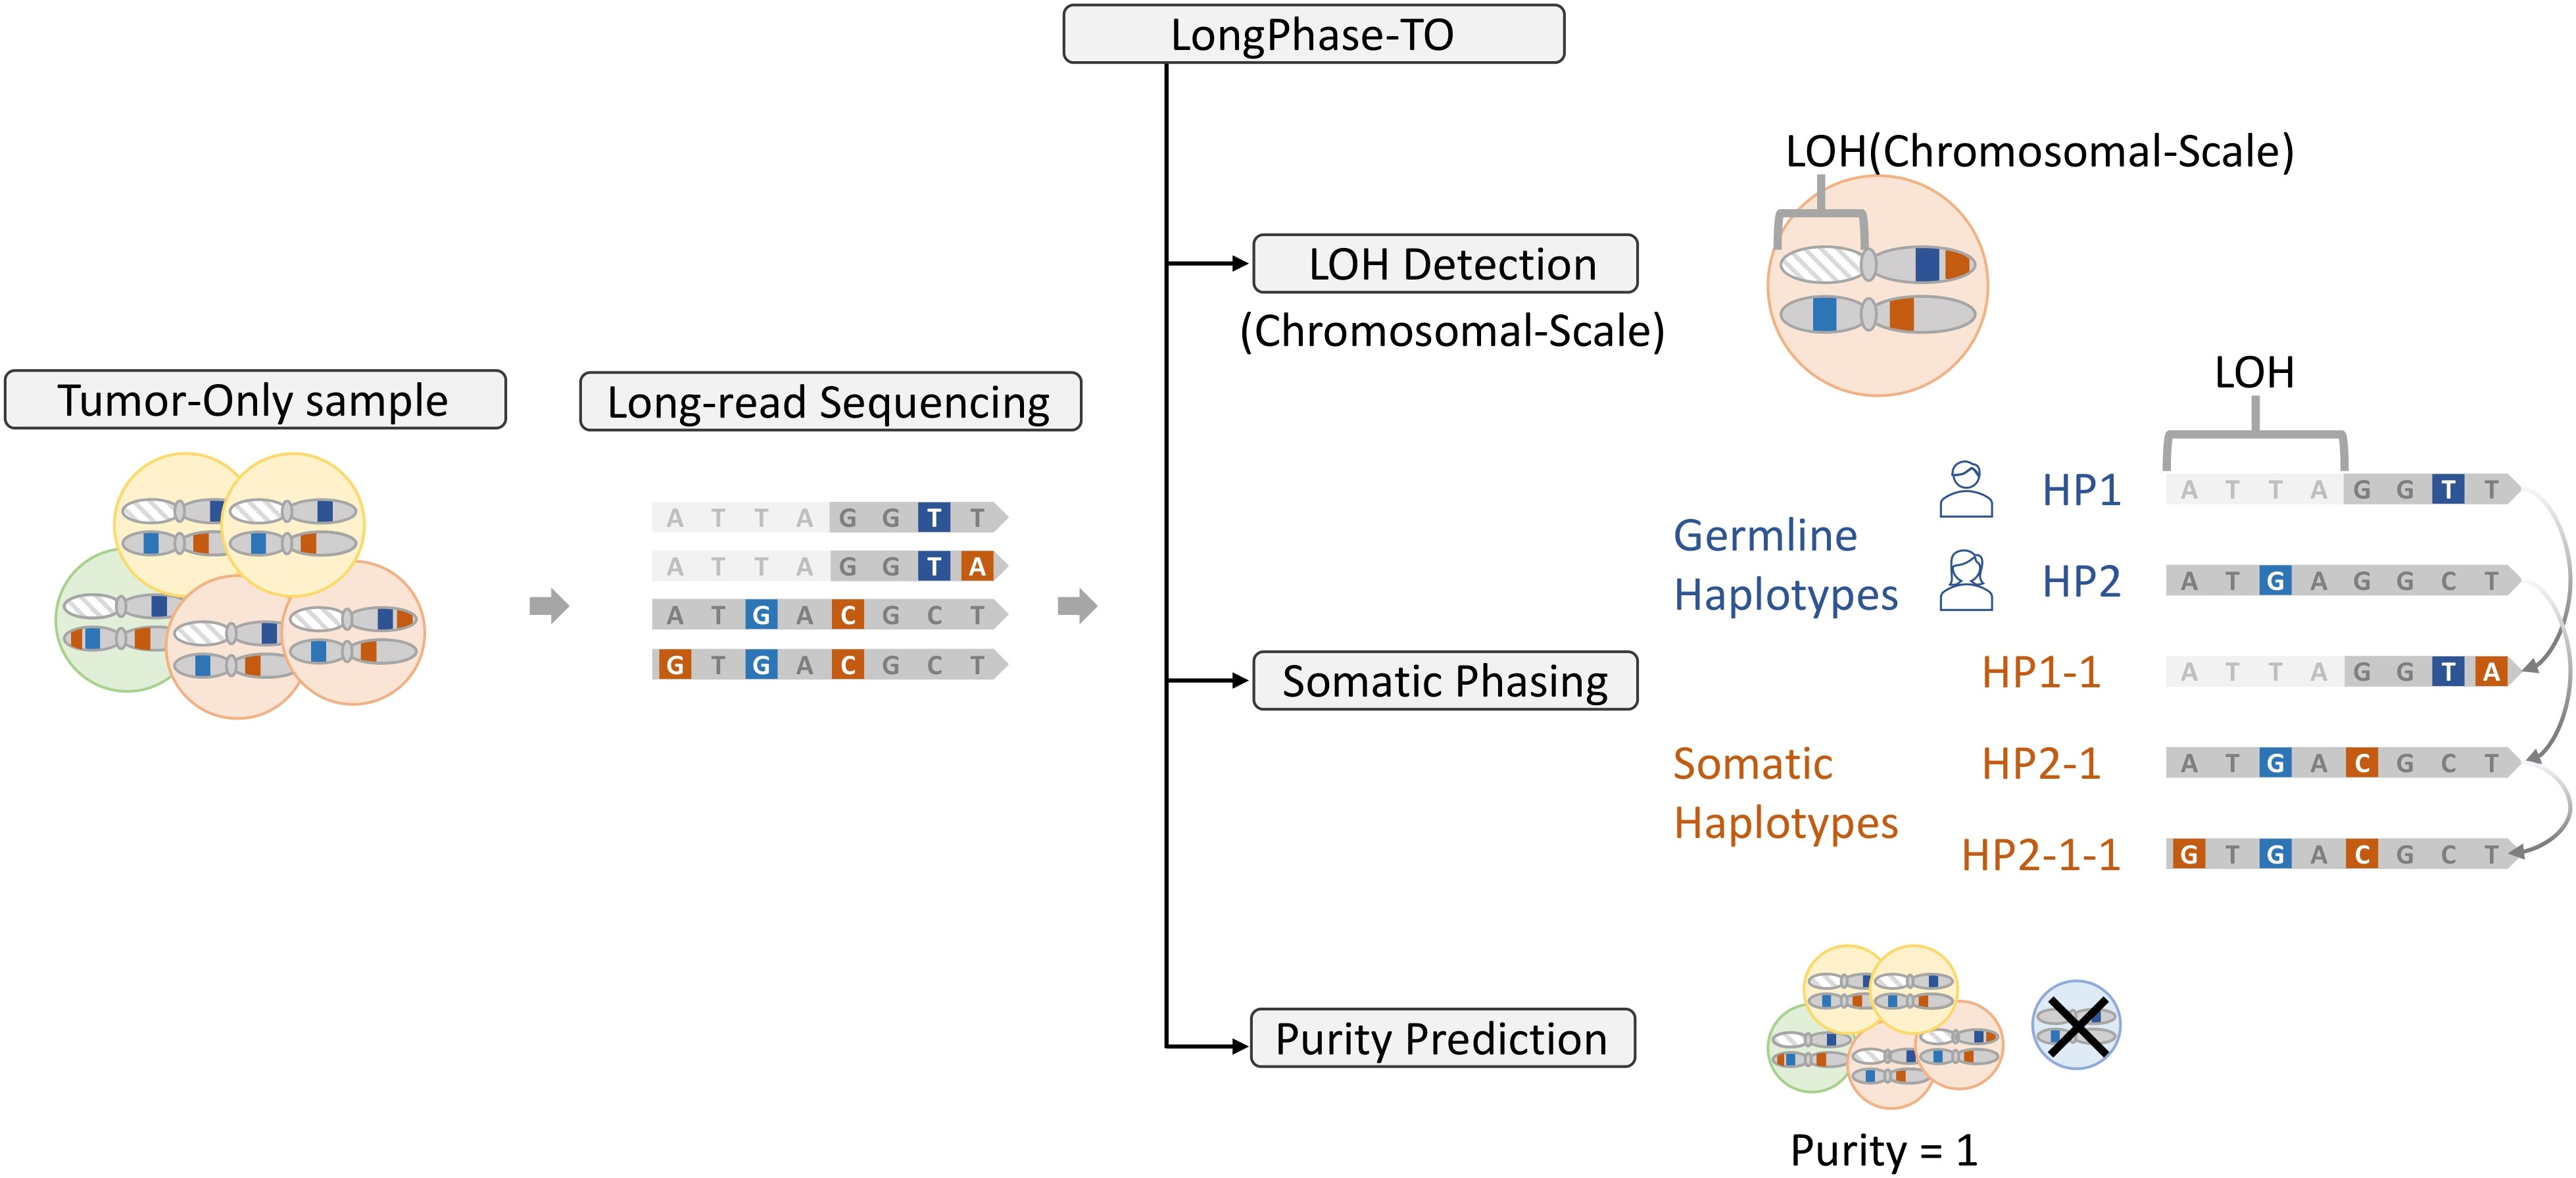
\includegraphics[keepaspectratio]{page_10_cropped.jpg}}
\caption[LongPhase-TO Pipeline Overview]{Flowchart illustrating the overall objective of the LongPhase-TO pipeline. The process starts with a heterogeneous tumor-only sample, which undergoes long-read sequencing. The resulting data is processed by the LongPhase-TO pipeline, which performs three core analyses: chromosome-scale LOH detection, somatic phasing to reconstruct germline and somatic haplotypes, and tumor purity prediction.}\label{fig:met-page-10-cropped-jpg}
\end{figure}

The pipeline is structured to process raw long-read sequencing data from a tumor sample and produce a detailed genomic profile of the cancer. This process encompasses three core analytical modules.

The analysis begins with chromosome-Scale Loss of Heterozygosity (LOH) Detection, which identifies large genomic regions where one of the two parental chromosome copies has been lost. This detection operates at the chromosome scale, enabling the characterization of major structural alterations.

The second module, Somatic Phasing, leverages long sequencing reads to perform phasing, assigning genetic variants to their parental chromosome of origin (haplotype). The pipeline first reconstructs the patient's two germline haplotypes and then identifies novel somatic haplotypes that emerged during tumor evolution through the accumulation of somatic mutations, thereby providing a haplotype-resolved view of the tumor's genetic lineage.

Finally, Tumor Purity Prediction estimates the proportion of cancerous cells within the bulk tumor sample. Tumor purity is a critical covariate for interpreting somatic variant allele frequencies and understanding the tumor microenvironment. It is derived from the relative abundance of the reconstructed germline and somatic haplotypes.

By combining these three analyses, LongPhase-TO aims to provide a detailed and accurate genomic portrait of a tumor from a single sample, offering insights into its clonal heterogeneity, evolutionary history, and structural landscape.

\subsection{Overview of the Analytical Workflow}\label{overview-of-the-analytical-workflow}

To achieve its objectives, the LongPhase-TO pipeline employs a structured, multi-step methodology designed to progressively refine raw sequencing data into a comprehensive genomic characterization. The workflow integrates several distinct analytical stages, each building upon the output of the previous one (Figure~\ref{fig:met-page-11-cropped-jpg}). The six primary steps are outlined below.

\begin{figure}
\centering
\pandocbounded{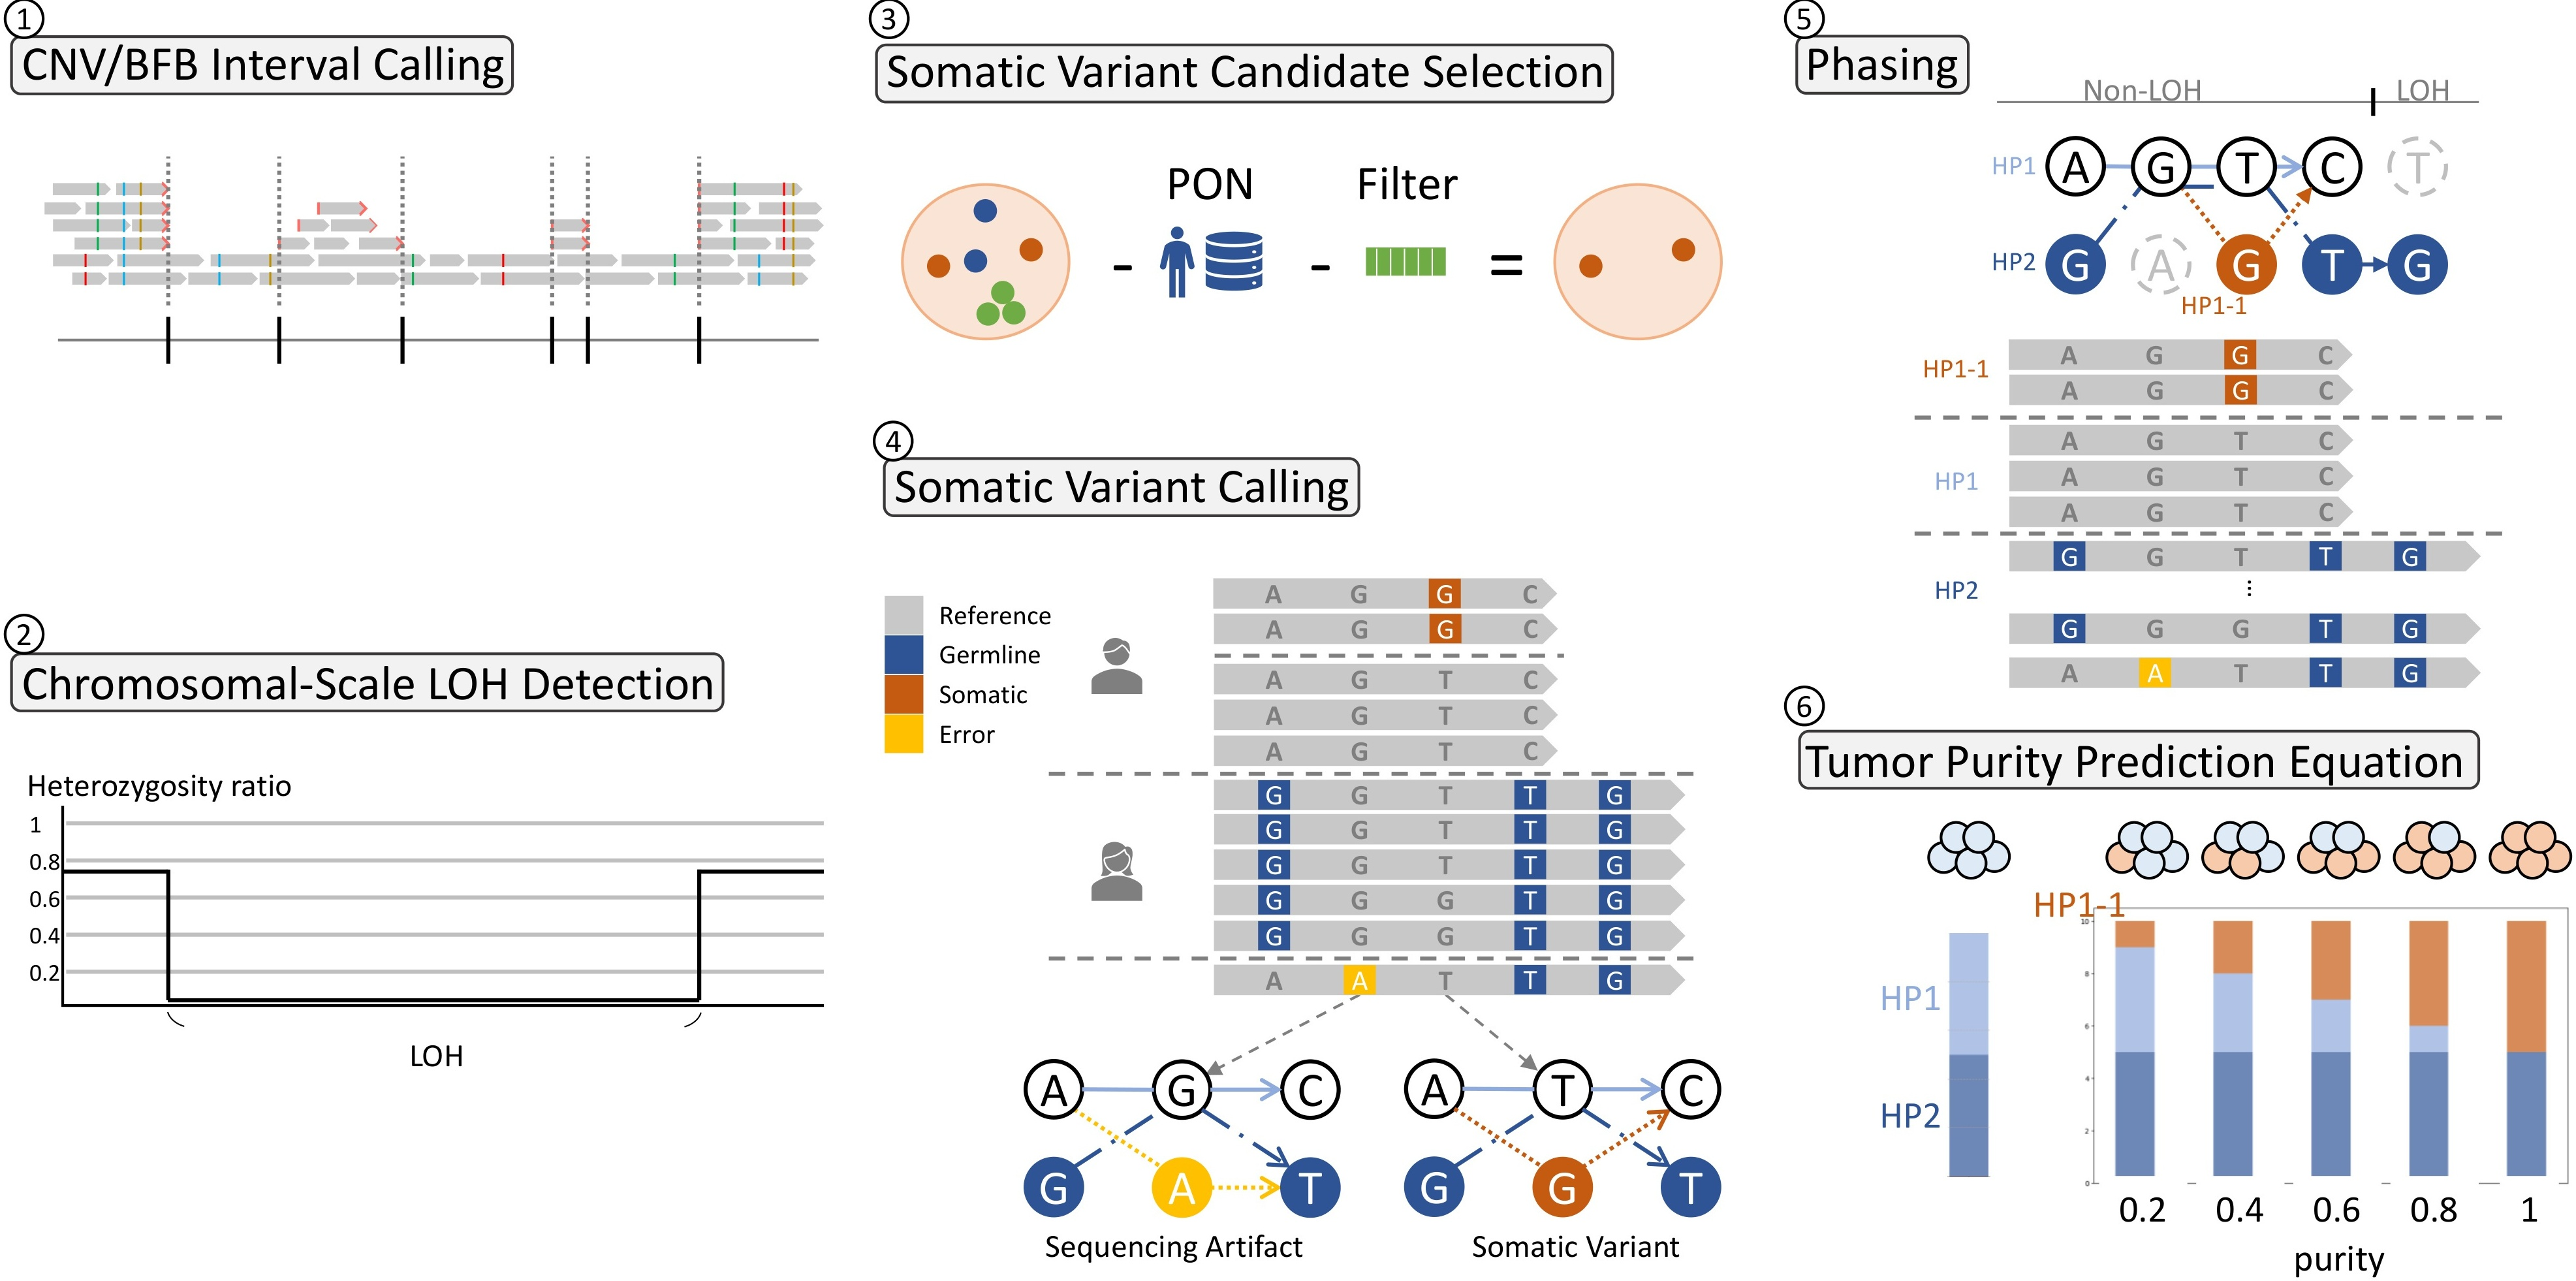
\includegraphics[keepaspectratio]{page_11_cropped.jpg}}
\caption[Six-Step Analytical Method]{Overview of the six-step analytical method. The workflow starts with (1) CNV/BFB interval calling, followed by (2) chromosome-scale LOH detection via heterozygosity ratio, (3) somatic variant candidate selection using a Panel of Normals, (4) graph-based somatic variant calling, (5) phasing of germline and somatic haplotypes, and concludes with (6) tumor purity prediction based on haplotype frequencies.}\label{fig:met-page-11-cropped-jpg}
\end{figure}

The analysis pipeline begins with a genome-wide screen for regions indicative of large-scale structural variations, termed CNV/BFB interval calling. This step involves analyzing the alignment patterns of long reads, particularly the locations of soft-clipped sequences, to identify candidate genomic intervals likely containing Copy Number Variations (CNVs) or complex rearrangements resulting from Breakage-Fusion-Bridge (BFB) cycles.

Using the information from this initial screen, the pipeline proceeds to chromosome-Scale LOH Detection, which focuses on identifying large regions of Loss of Heterozygosity (LOH). The method quantifies the ratio of heterozygous to homozygous variants across the genome, and a significant, sustained drop in this ratio over an extended chromosome segment is interpreted as an LOH event, signifying the loss of one parental allele.

To confidently identify tumor-specific mutations without a matched normal sample, the workflow next performs Somatic Variant Candidate Selection. An initial set of all detected variants is filtered against a Panel of Normals (PON), a comprehensive database of common germline variants and recurrent sequencing artifacts. This subtractive filtering enriches the candidate pool for high-confidence somatic mutations by removing known polymorphisms.

The refined set of candidates is then subjected to Somatic Variant Calling, which employs a novel graph-based approach to model local haplotype structures. By analyzing the linkage of variants on the same long reads, the method distinguishes true, low-frequency somatic variants that form consistent new haplotypes from sporadic sequencing errors.

In the Phasing step, the pipeline reconstructs the full-length haplotypes present in the sample, assigning identified somatic and germline variants to their respective chromosomes of origin. This resolves the two primary germline haplotypes (HP1 and HP2) and also identifies novel somatic haplotypes that have evolved from the germline state (e.g., HP1-1 derived from HP1). Information from the LOH detection step is integrated to correctly model haplotype composition in regions affected by allelic loss.

Finally, Tumor Purity Prediction leverages the quantitative output of the phasing module to estimate tumor purity. The relative frequencies of reconstructed germline and somatic haplotypes serve as input to a predictive model; as tumor purity increases, the abundance of somatic haplotypes relative to their germline counterparts rises in a predictable manner, enabling an accurate purity score to be calculated.

This integrated workflow ensures that each analytical component informs the others, leading to a robust and detailed characterization of the tumor genome from a single long-read sequencing experiment.

\subsection{CNV and BFB Interval Calling}\label{cnv-and-bfb-interval-calling}

The identification of genomic intervals affected by large structural variants, such as CNVs and BFB-induced rearrangements, is a critical first step in characterizing the tumor genome. The method accomplishes this by systematically analyzing clipping patterns in long-read sequencing alignments. Clipping occurs when a portion of a sequencing read does not align to the reference genome, often because the read spans a structural variant breakpoint.

\subsubsection{Principle of Clipping Pattern Analysis}\label{principle-of-clipping-pattern-analysis}

The alignment of long reads across structural variant breakpoints generates characteristic and non-random patterns of clipping, including both soft and hard clipping. These patterns, encoded in the CIGAR (Compact Idiosyncratic Gapped Alignment Report) string of an alignment file, serve as informative signatures for specific SV types. A CIGAR string such as \texttt{10S5M2D1M} indicates that the first 10 bases of the read were soft-clipped (\texttt{10S}), followed by 5 matching bases (\texttt{5M}), a 2-base deletion (\texttt{2D}), and one additional matching base (\texttt{1M}).

Distinct SVs produce unique spatial arrangements of these clipping types. For instance, a tandem duplication often presents as a sharp peak of up-clipped reads immediately followed by a sharp peak of down-clipped reads at the duplication boundaries. A fold-back inversion, a hallmark of BFB cycles, can produce a more complex signature of alternating and overlapping up-clipping and down-clipping signals. The algorithm is designed to computationally detect and delineate these signature-rich intervals.

\subsubsection{Algorithmic Detection of Clipping Signatures}\label{algorithmic-detection-of-clipping-signatures}

The formal identification of CNV and BFB intervals is performed using a three-step signal processing algorithm that transforms raw alignment data into defined genomic regions.

\paragraph{Clipping Breakpoint Extraction and Quantification}\label{clipping-breakpoint-extraction-and-quantification}

The algorithm first parses the alignment file (e.g., BAM format) for every clipped read. For each clipped read, the genomic coordinate of the clipping breakpoint is recorded. To create a directional signal, up-clipping events are assigned a positive value (e.g., +1) and down-clipping events are assigned a negative value (e.g., -1). This process converts the spatial distribution of clipped reads into a quantitative scatter plot of Clipping Count versus genomic position, where each point represents the net clipping signal at a single base (Figure~\ref{fig:met-page-14-cropped-jpg}).

\begin{figure}
\centering
\pandocbounded{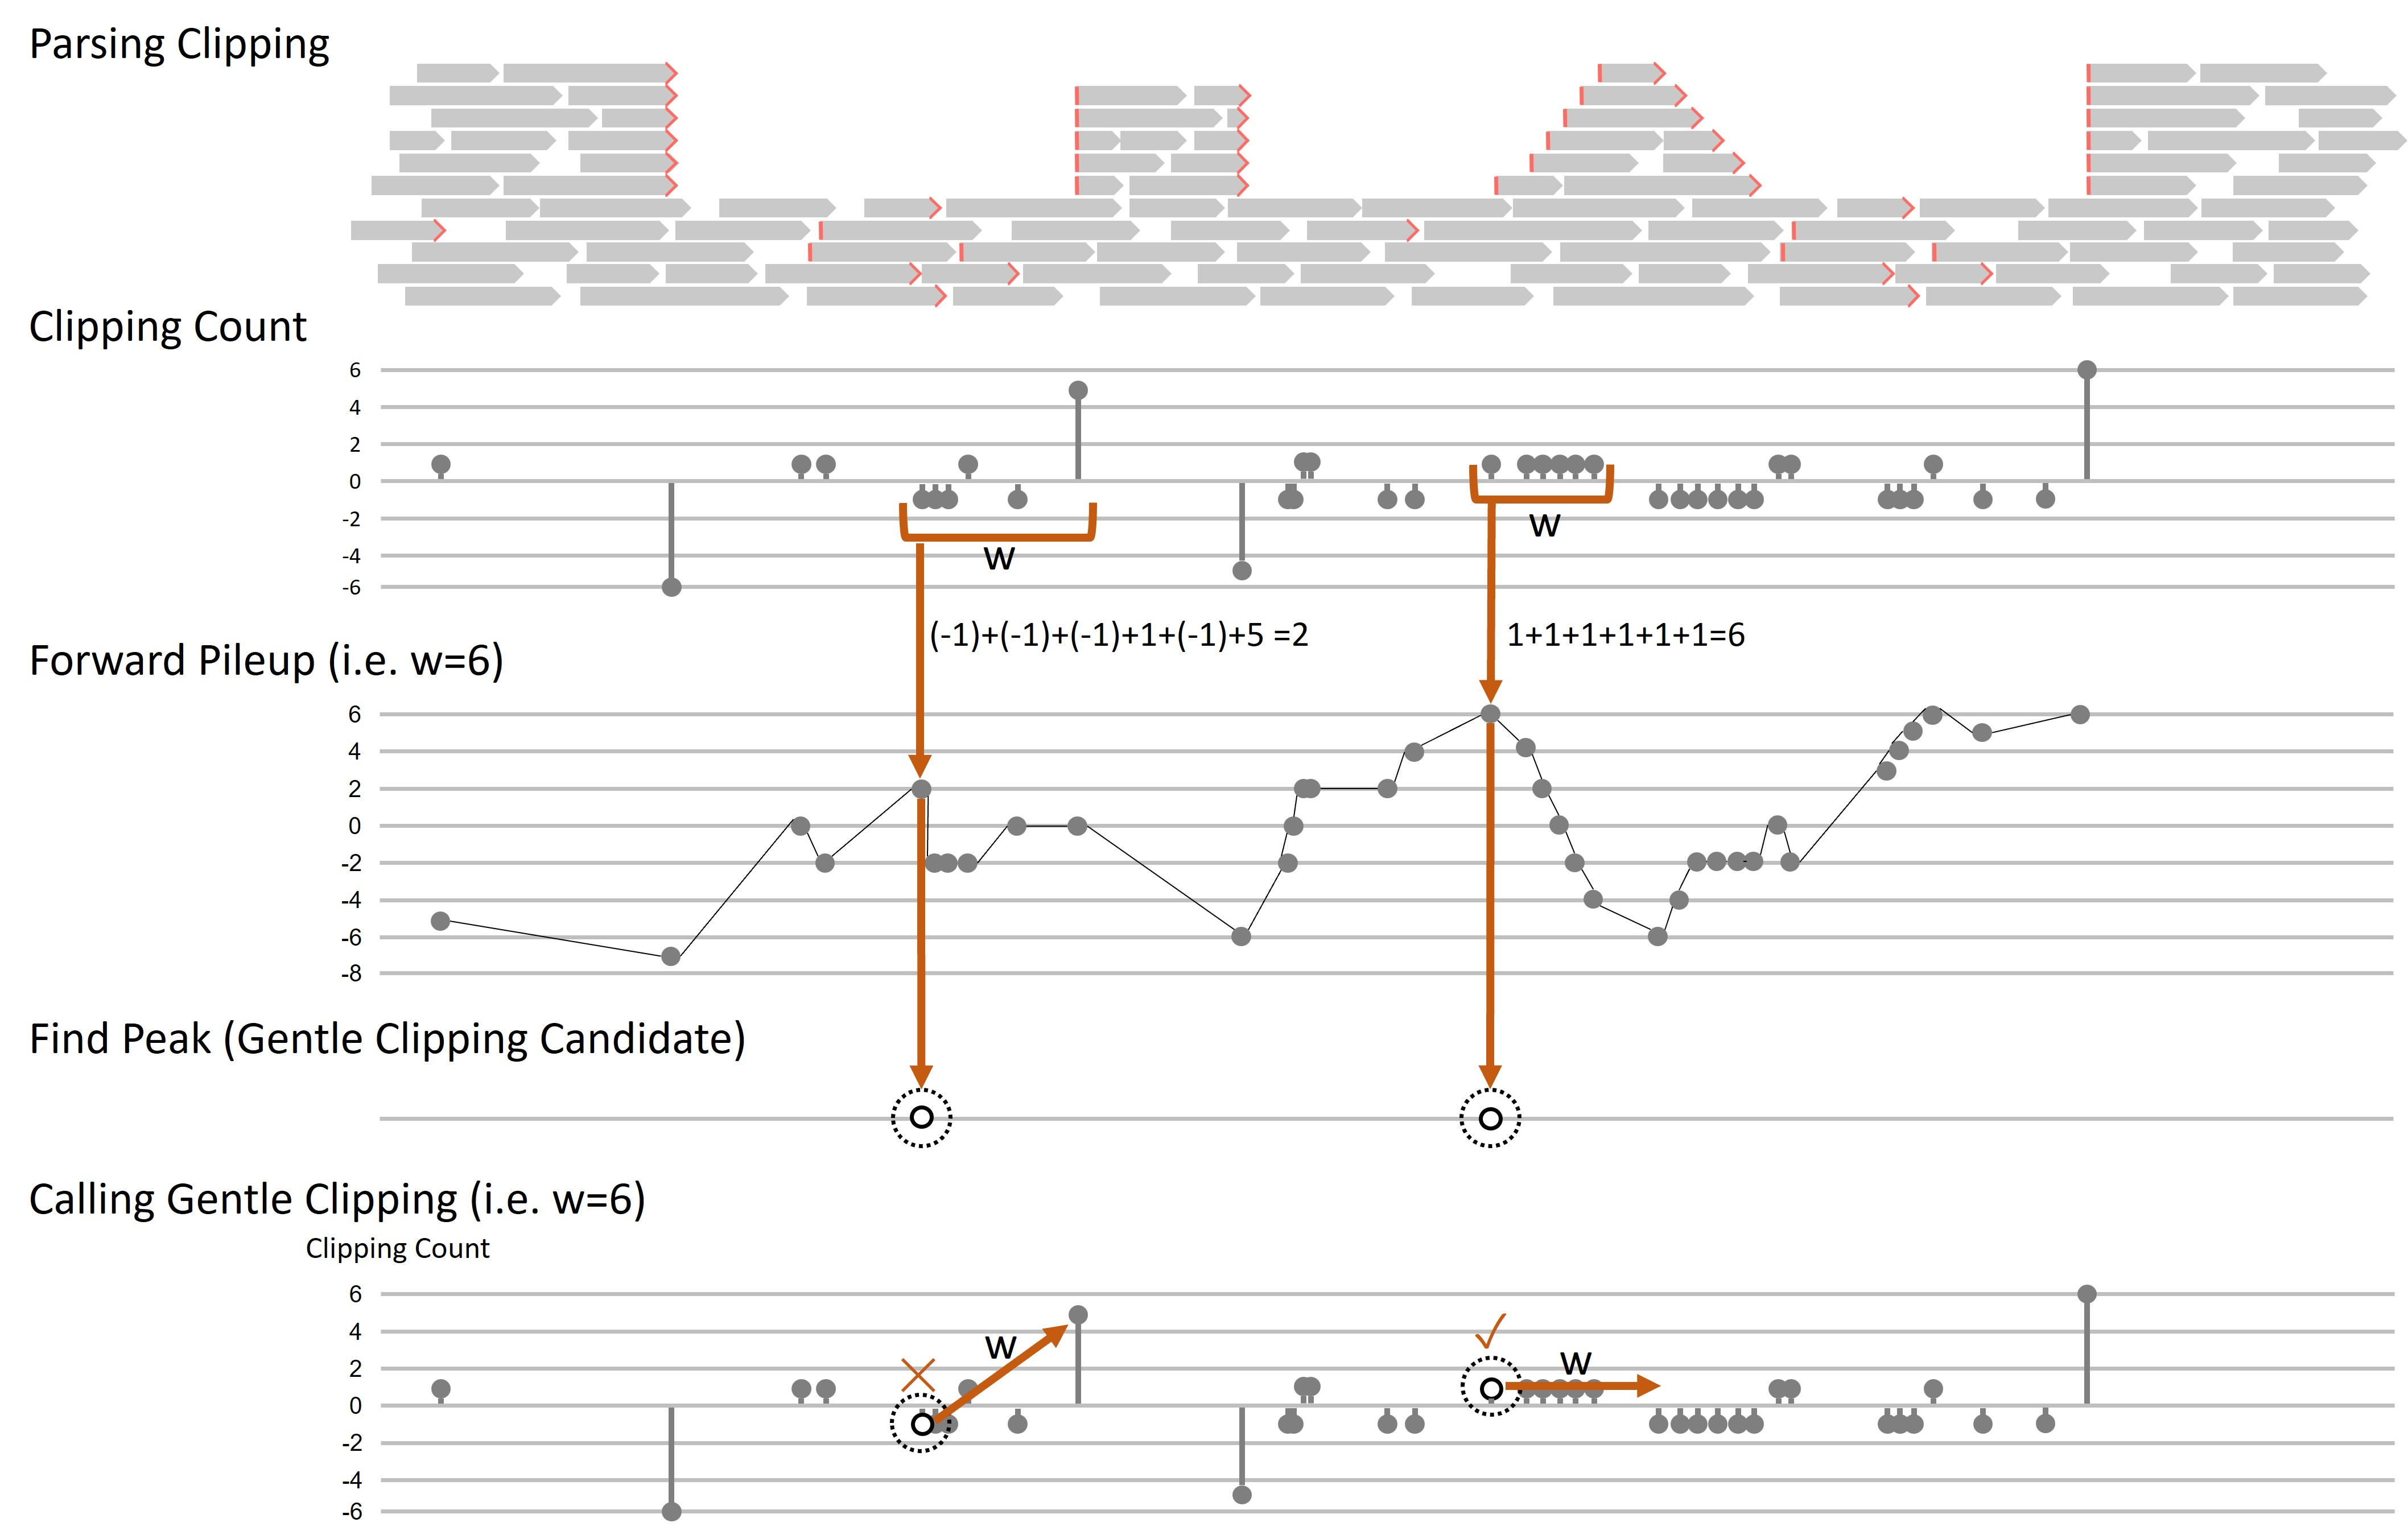
\includegraphics[keepaspectratio]{page_14_cropped.jpg}}
\caption[Clipping Breakpoint Detection and Gentle Clipping Identification]{The alignment file is parsed to extract clipped reads, and the breakpoint positions are transformed into directional clipping signals (Clipping Count). A sliding window summation (Forward Pileup, e.g., w=6) is applied to smooth the signal, enhancing consecutive low-amplitude events into discernible peaks. Peaks in the Forward Pileup profile are identified as candidate Gentle Clipping regions. To reduce false positives arising from isolated high-amplitude events, an additional filtering step is performed, ensuring that only regions characterized by sustained accumulative signals are retained as genuine Gentle Clipping events.
}\label{fig:met-page-14-cropped-jpg}
\end{figure}

\paragraph{Gentle Clipping Signal Enhancement}\label{gentle-clipping-signal-enhancement}

Simple peak detection on the clipping count signal is insufficient to capture all relevant SV features. Therefore, an advanced feature detection strategy is introduced, specifically targeting gentle clipping, which refers to low amplitude but persistently occurring clipping events, and implemented through two consecutive steps for detection and signal quantification.

\subparagraph{Gentle Clipping Boundary Identification}

This criterion targets regions with a high density of consistent, low-amplitude clipping events rather than isolated high peaks. The signal is often sparse and noisy; to enhance true signals and reduce noise, detection begins with a smoothing step using a sliding window summation, termed Forward Pileup. For a window of size \texttt{w}, the pileup value is the sum of clipping counts within that window, e.g., \texttt{[1,1,1,1,1,1]} yields 6, while \texttt{[-1,-1,-1,1,-1,5]} yields 2. This process transforms the discrete scatter plot into a continuous signal profile, amplifying sustained clipping events into distinct peaks and valleys (Figure~\ref{fig:met-page-14-cropped-jpg}).

The onset of a Gentle Clipping region can be located by identifying peaks in the Forward Pileup profile. Owing to its cumulative nature, a high pileup value indicates that subsequent positions predominantly contribute positive increments. When the signal transitions from sustained increase to decrease, the pileup value correspondingly drops, making the peak a reliable marker for the start of a Gentle Clipping event (Figure~\ref{fig:met-page-14-cropped-jpg}).

However, a single high-amplitude clipping event within the window \texttt{w} can also yield a large Forward Pileup value, potentially mimicking the signal of Gentle Clipping. To prevent such false positives, an additional filtering step is applied to determine whether the elevated pileup value is caused by a single high peak or by a genuine accumulation of multiple low-level events. This distinction ensures that only sustained, high-density clipping regions are classified as Gentle Clipping candidates (Figure~\ref{fig:met-page-14-cropped-jpg}).

Similarly, the termination of a Gentle Clipping region can be identified by applying the same procedure in reverse. In this case, the Forward Pileup is replaced with a Reverse Pileup computation, and the peak detection logic is applied to points where the signal transitions from a positive to a negative trend. This corresponds to regions where the cumulative value exhibits a sustained decrease and reaches a local minimum, marking the boundary at which the Gentle Clipping event ends. This symmetric detection framework ensures that both the onset and termination of Gentle Clipping regions are delineated in a consistent and accurate manner.


\subparagraph{Gentle Clipping Amplitude Quantification}

To improve the interpretability of identified Gentle Clipping sites, an amplification step that quantifies the relative magnitude of local signal variation. This process begins by constructing a Clipping Pileup profile, derived from summing the raw Clipping Count values for each genomic coordinate, thereby preserving both the directionality and magnitude of clipping events.

For each Gentle Clipping candidate, two reference points are defined: one located w bases upstream and the other w bases downstream of the candidate position, where w corresponds to the predefined window size used in the Forward Pileup procedure. The Clipping Pileup values at these two positions are then retrieved, and their difference is calculated to quantify the local amplitude of change (Figure~\ref{fig:met-page-15-cropped-jpg}).

A higher amplitude value denotes a more pronounced and abrupt transition in the clipping signal, indicative of a stronger and more distinct breakpoint signature. This quantitative metric is retained for downstream analyses to guide the identification of breakpoint-associated genomic intervals.

\begin{figure}
\centering
\pandocbounded{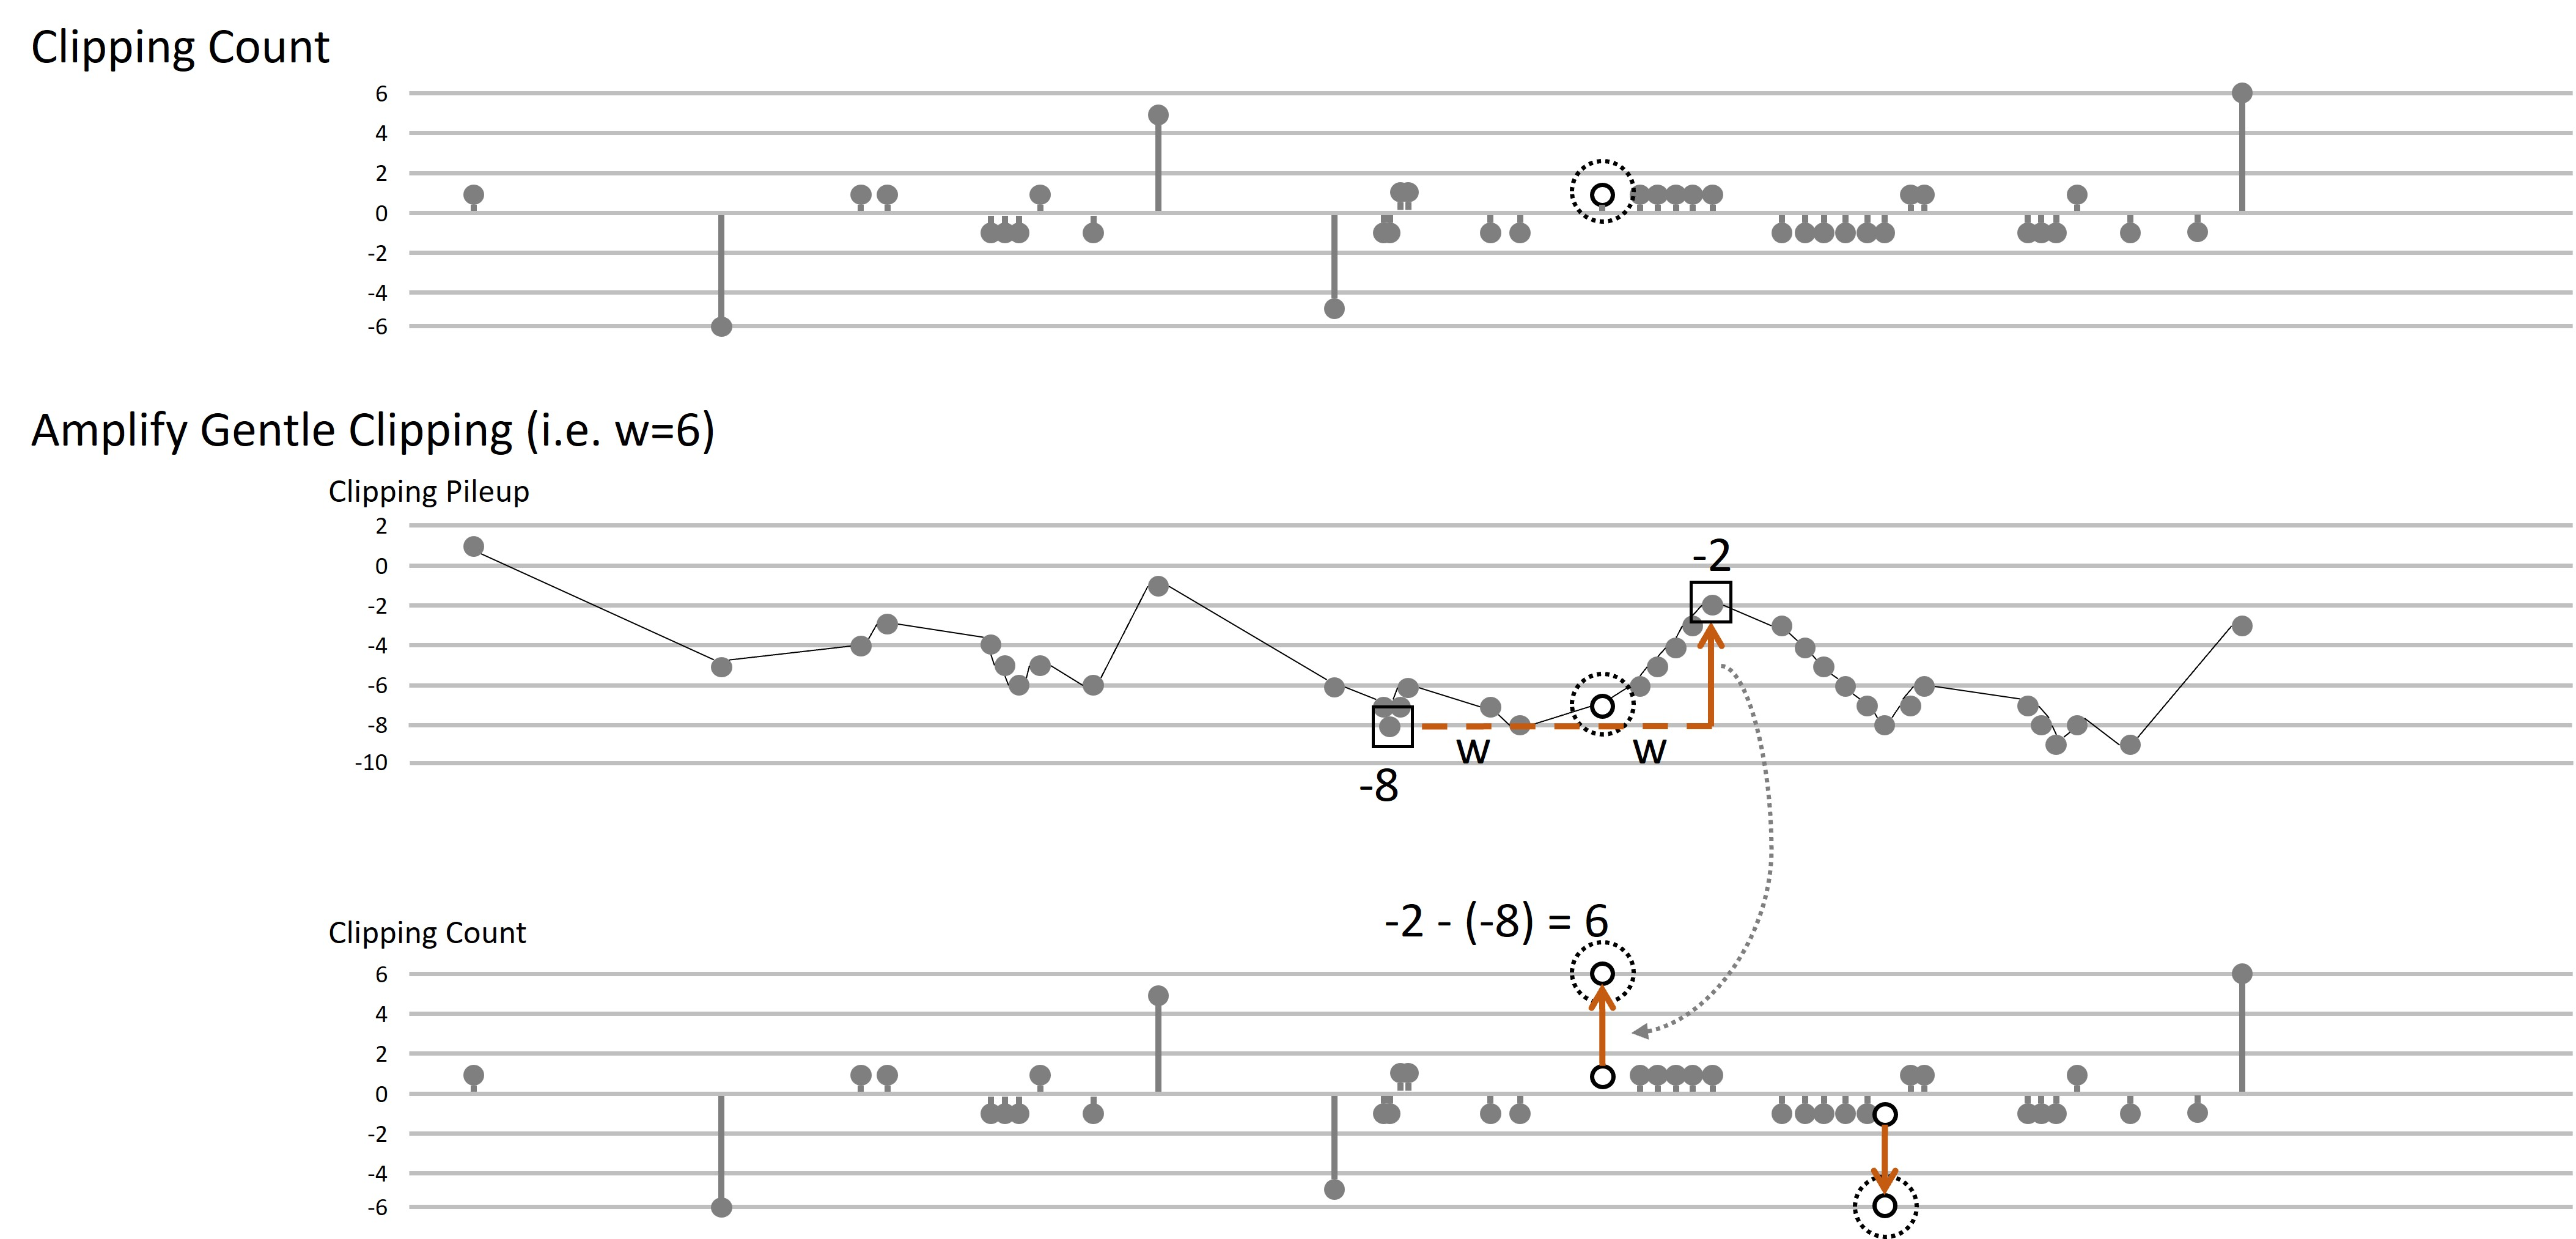
\includegraphics[keepaspectratio]{page_15_cropped.jpg}}
\caption[Amplification of Gentle Clipping Signal]{Illustration of the amplification procedure for Gentle Clipping signal quantification. The raw clipping counts are first aggregated into a Clipping Pileup profile, which retains both the directionality and magnitude of clipping events. For each Gentle Clipping candidate, two reference points are selected at positions $w$ bases upstream and downstream, where $w$ corresponds to the predefined sliding window size. The Clipping Pileup values at these reference positions are compared, and their difference is computed to measure the local signal amplitude, thereby improving the interpretability of Gentle Clipping sites.}\label{fig:met-page-15-cropped-jpg}
\end{figure}


\paragraph{Breakpoint-Guided Interval Calling}\label{breakpoint-guided-interval-calling}

Following the Advanced Signal Feature Detection step, the signal amplitudes from the Gentle Clipping process are further enhanced, ensuring that low-intensity fluctuations no longer contain features of interest. Consequently, signal components with amplitudes below the threshold $\lambda$ can be confidently discarded, while retaining only the prominent signal peaks that represent meaningful biological events.


Following this noise reduction, the core detection mechanism relies on the concept of Signal Swing, which is defined by two complementary conditions that assess both signal similarity and spatial proximity. For a pair of signal points \(i\) and \(j\) with clipping pileup values \(c_i\) and \(c_j\) respectively, a signal swing is identified when these points satisfy the following criteria:

\[
(c_i / c_j \ge \alpha) \land (|j - i| \le \beta)
\]

The first condition, \(c_i / c_j \ge \alpha\), evaluates the ratio of signal amplitudes to determine whether the two points exhibit similar signal characteristics, where $\alpha$ represents the minimum amplitude ratio threshold. The second condition, \(|j - i| \le \beta\), ensures spatial proximity by constraining the maximum genomic distance between the signal points to $\beta$ base pairs.

The genomic coordinates derived from validated signal swings serve as the boundaries for distinguishing between larger genomic intervals and smaller regions, enabling precise identification of CNV and BFB candidate regions (Figure~\ref{fig:met-page-16-cropped-jpg}).


\begin{figure}
\centering
\pandocbounded{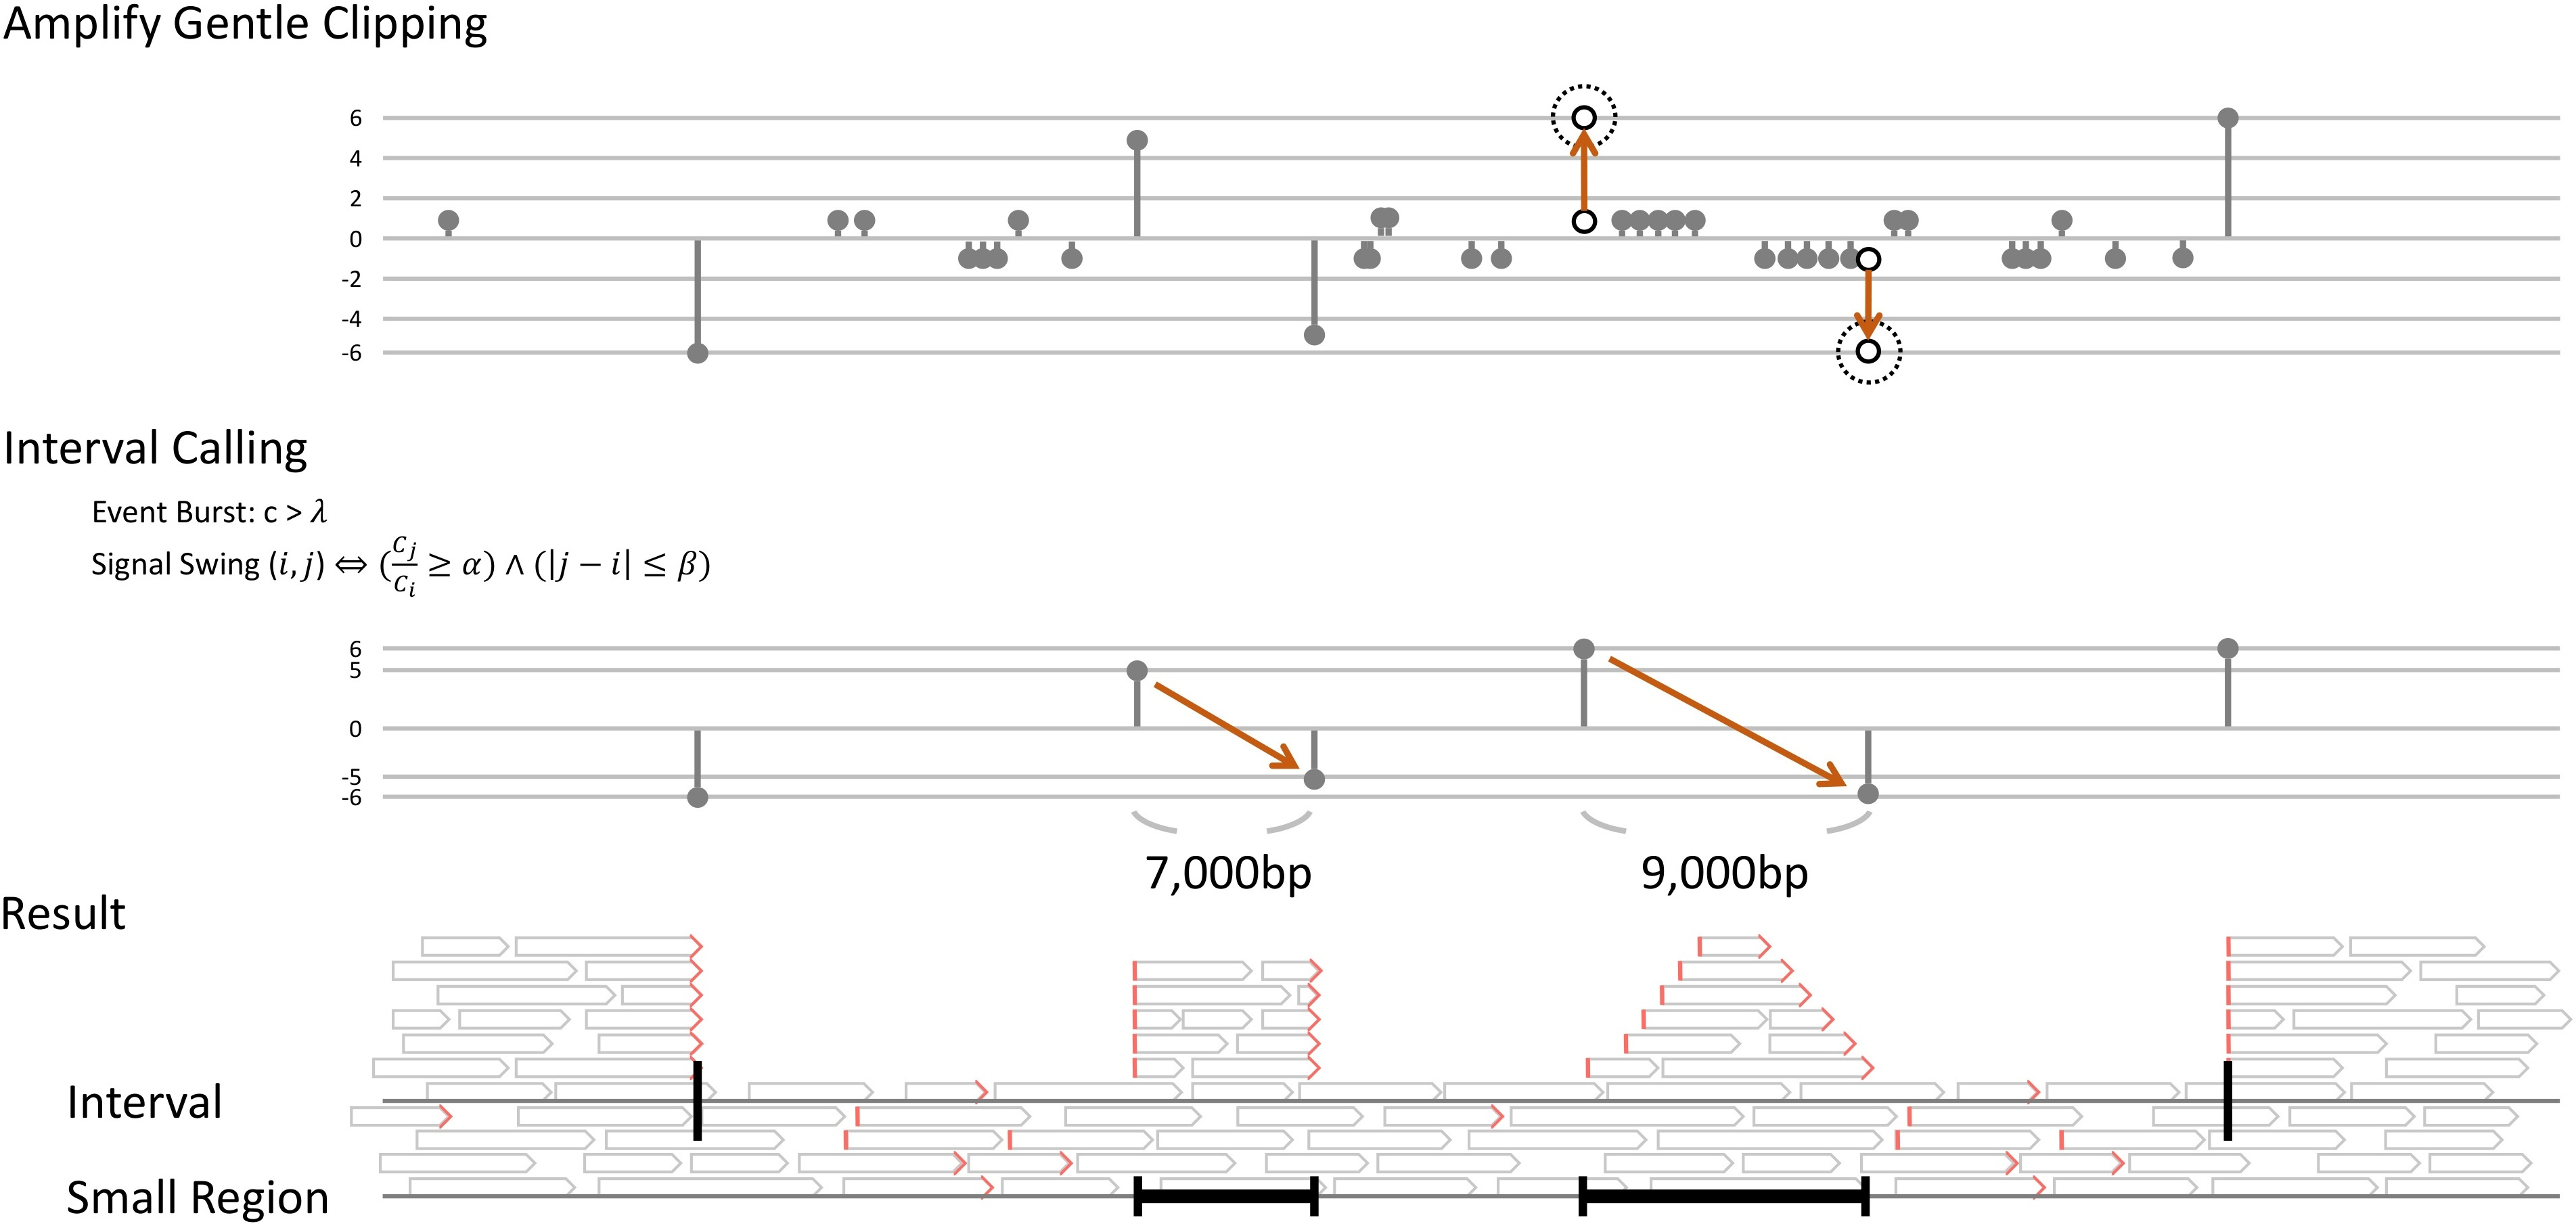
\includegraphics[keepaspectratio]{page_16_cropped.jpg}}
\caption[Breakpoint-Guided Interval Calling]{Only prominent clipping signal peaks are retained after signal enhancement, and genomic intervals are subsequently identified based on combined constraints of signal amplitude and spatial distance. The resulting genomic coordinates define the boundaries of intervals and sub-regions, enabling precise detection of candidate CNV and BFB regions.}\label{fig:met-page-16-cropped-jpg}
\end{figure}

\subsection{Chromosome-Scale Loss of Heterozygosity Detection}\label{chromosome-scale-loss-of-heterozygosity-detection}

Loss of Heterozygosity (LOH) is a hallmark of cancer genomes, reflecting the loss of one parental allele over a large genomic region. LOH events are detected at a chromosome scale by integrating variant information with the previously identified CNV and BFB intervals.

\subsubsection{LOH Detection via Heterozygosity Ratio}\label{loh-detection-via-heterozygosity-ratio}

The primary signal for LOH is a stark imbalance in allelic ratios at heterozygous variant sites. For each known heterozygous single nucleotide variant (SNV), a heterozygosity ratio is calculated based on the read counts supporting the heterozygous versus homozygous state. This is defined as:

\[
\text{Heterozygosity ratio} = \frac{\text{Het Count}}{\text{Het Count} + \text{Hom Count}}
\]

In a normal diploid region, this ratio is expected to be close to 1.0 (or a high value, accounting for mapping biases). In a region of LOH, where one allele is lost, the vast majority of reads will support the remaining allele, causing the heterozygosity ratio to drop to a value near zero. An LOH event is called if this ratio falls below a predefined threshold, $\sigma$:

\[
\text{Heterozygosity ratio} < \sigma
\]

Visually, this corresponds to the complete disappearance of long reads supporting one of the two haplotypes over a large genomic span.

\subsubsection{Merging LOH Segments for chromosome-Scale Analysis}\label{merging-loh-segments-for-chromosome-scale-analysis}

A key challenge in LOH detection is that large LOH regions can be interrupted by small, localized genomic events such as tandem duplications (CNVs) or complex rearrangements from BFB cycles. These events can locally restore a heterozygous state or create complex copy number profiles, causing transient spikes in the heterozygosity ratio and fragmenting the LOH call.

To accurately identify true, contiguous chromosome-scale LOH events under these circumstances, this method incorporates a critical filtering and merging step that explicitly leverages CNV and BFB intervals obtained in the previous stage. Without integrating these previously identified regions, large LOH segments could be fragmented by such small, localized events, making it impossible to recover the complete chromosome-scale pattern. During computation, the algorithm deliberately skips over these small, intervening genomic events to preserve the major, uninterrupted LOH span (Figure~\ref{fig:met-page-17-cropped-jpg}), enabling the reconstruction of a single, continuous LOH event that provides a more biologically accurate representation of a major chromosome alteration than treating it as multiple disjointed smaller events.

\begin{figure}
\centering
\pandocbounded{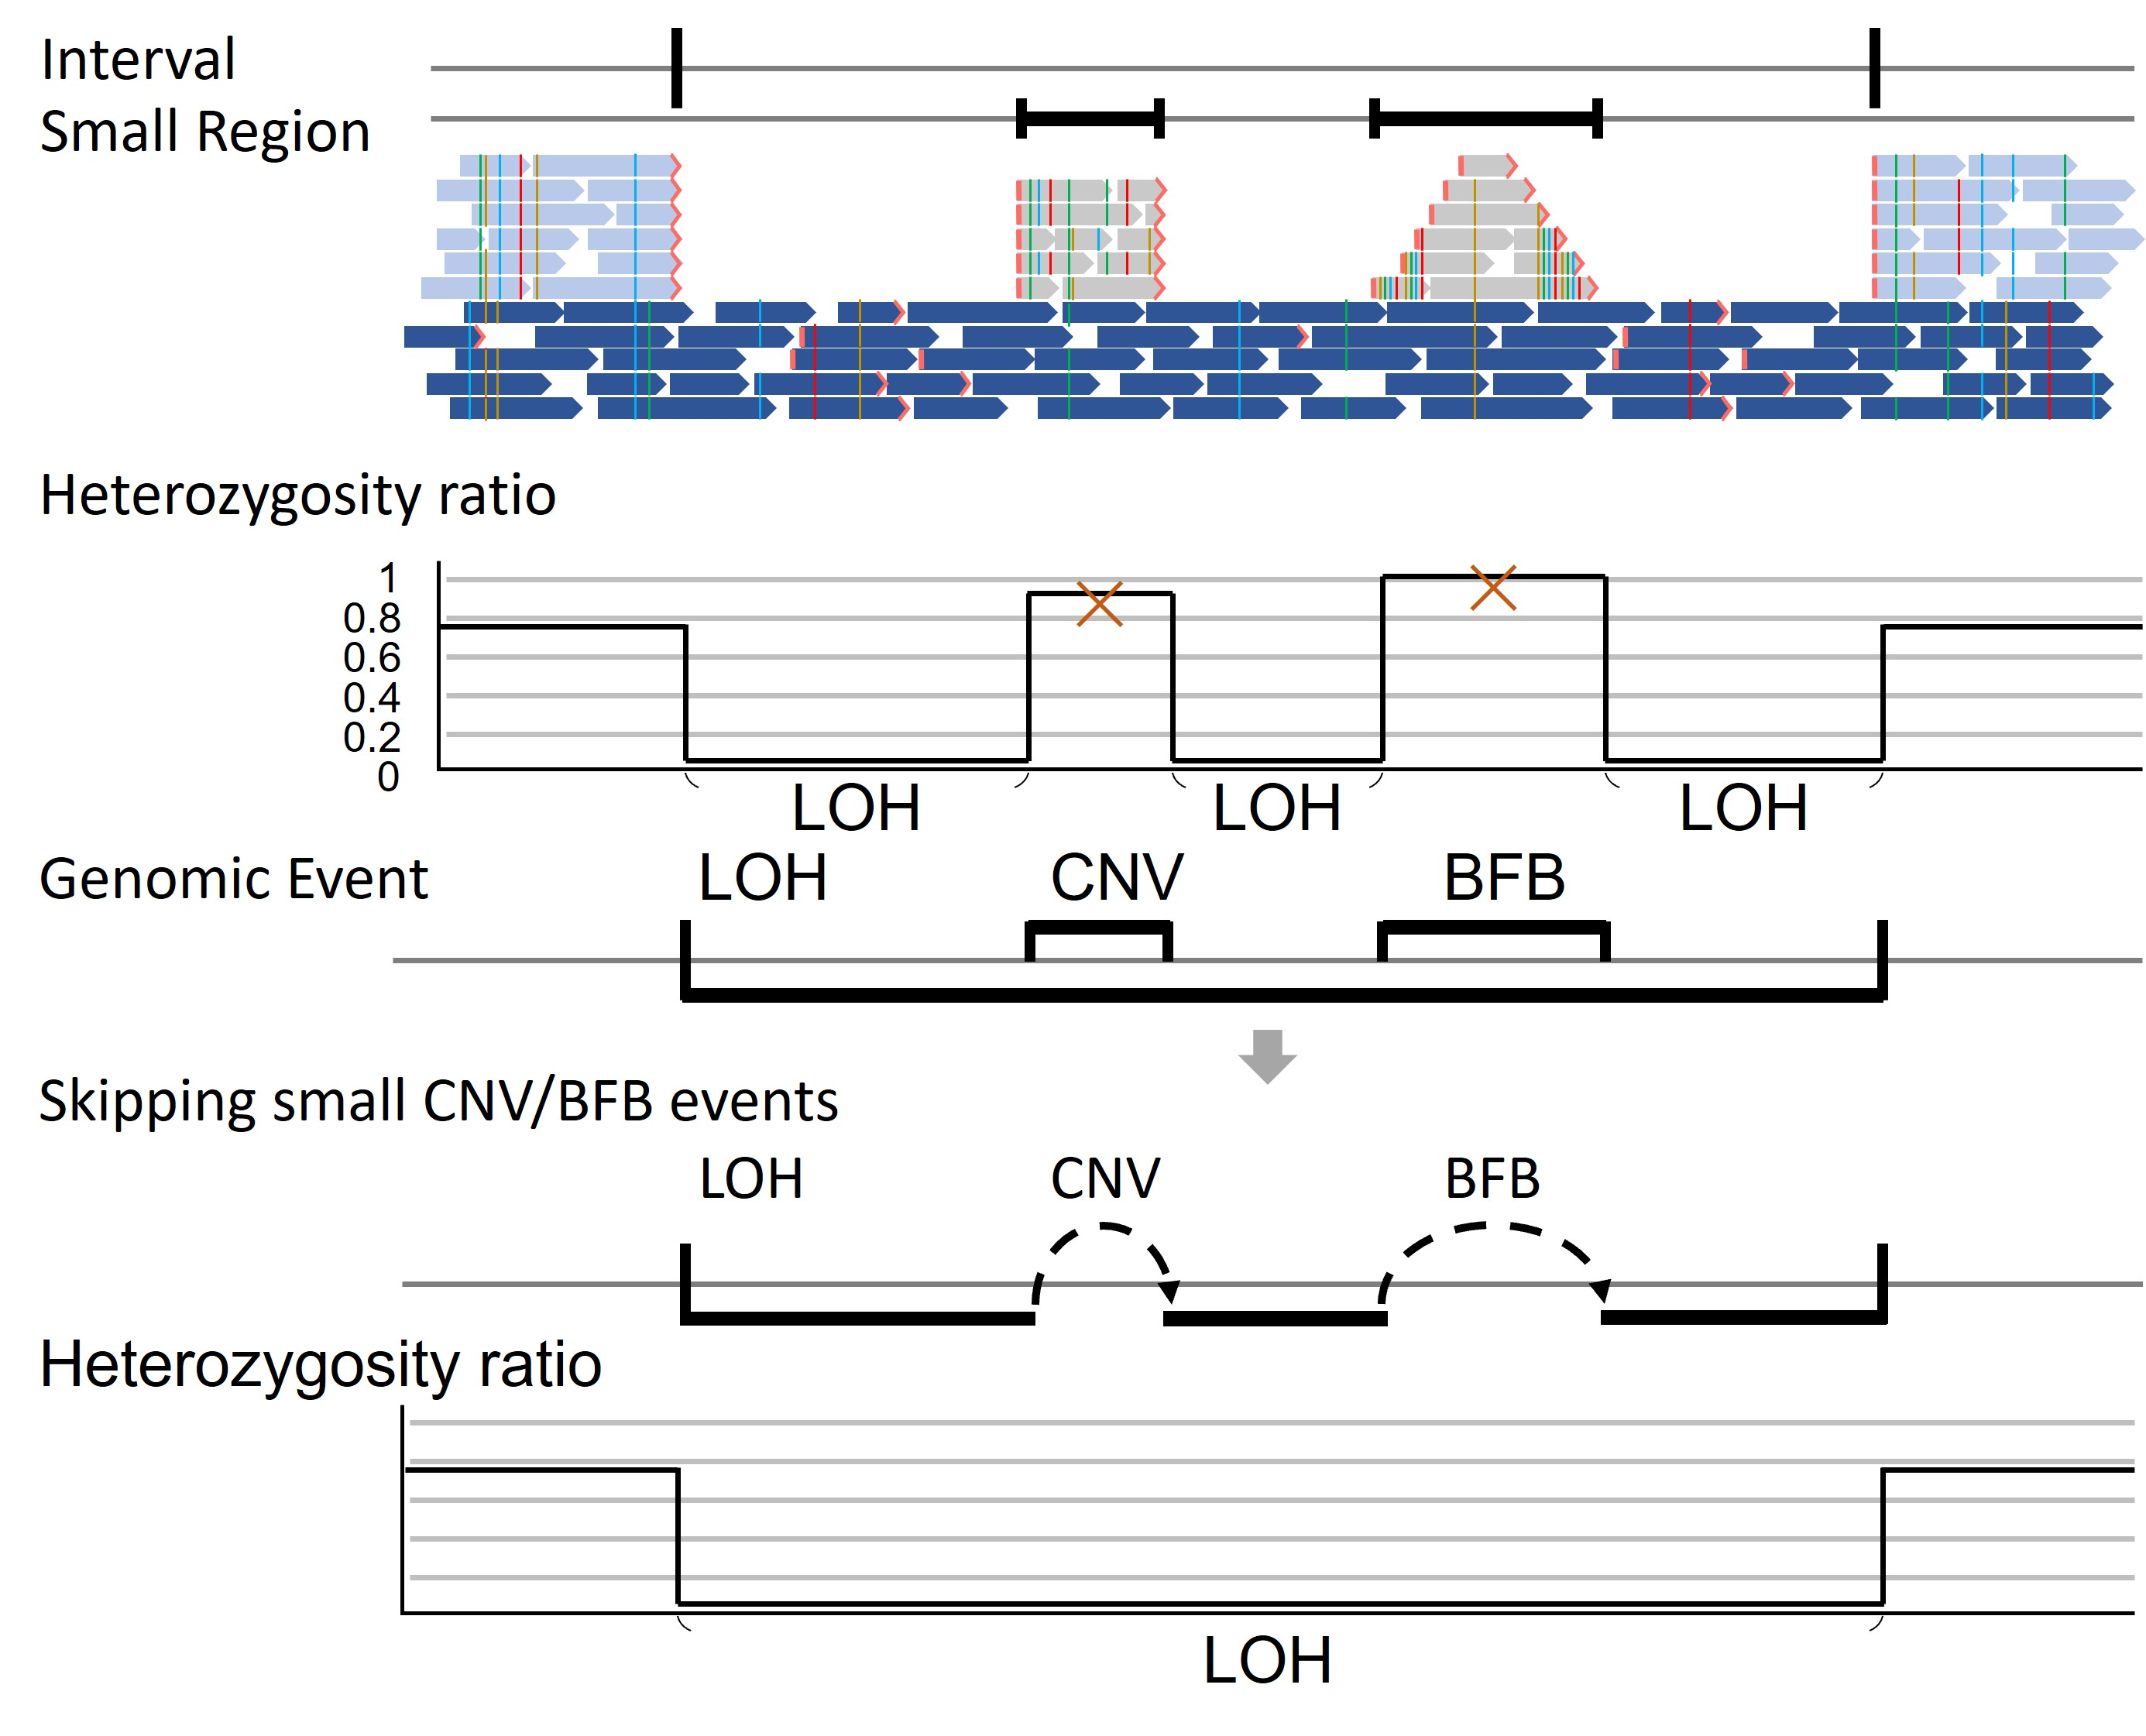
\includegraphics[width=0.8\textwidth, keepaspectratio]{page_17_cropped.jpg}}
\caption[Chromosome-scale LOH Detection]{Method for chromosome-scale LOH detection. The workflow shows that an initial pass may identify fragmented LOH regions interrupted by small CNV or BFB events that locally restore heterozygosity. The final step involves a merging process that filters out these small intervening events to define a single, continuous, large-scale LOH region.}\label{fig:met-page-17-cropped-jpg}
\end{figure}

\subsection{Somatic Variant Identification and Phasing}\label{somatic-variant-identification-and-phasing}

The accurate identification of somatic variants from tumor-only long-read data requires a multi-stage process that combines rigorous filtering, advanced haplotype-aware variant calling, and high-resolution phasing.

\subsubsection{Somatic Variant Candidate Selection}\label{somatic-variant-candidate-selection}

The initial list of variant candidates produced by a standard caller is a heterogeneous mixture of true somatic mutations, common germline variants, and technical artifacts. The first step is to enrich this list for true somatic events.

\paragraph{Filtering Against a Panel of Normals (PON)}\label{filtering-against-a-panel-of-normals-pon}

In the absence of a matched normal sample, a Panel of Normals (PON) is used to filter out common germline variants. The PON is a comprehensive database constructed from a large cohort of healthy individuals (e.g., 1000 Genomes Project, gnomAD) and also includes recurrent, technology-specific artifacts. All variant candidates from the tumor sample that are present in the PON are removed in a subtractive process that effectively eliminates the majority of non-somatic variants (Figure~\ref{fig:met-page-18-cropped-jpg}).

\begin{figure}
\centering
\pandocbounded{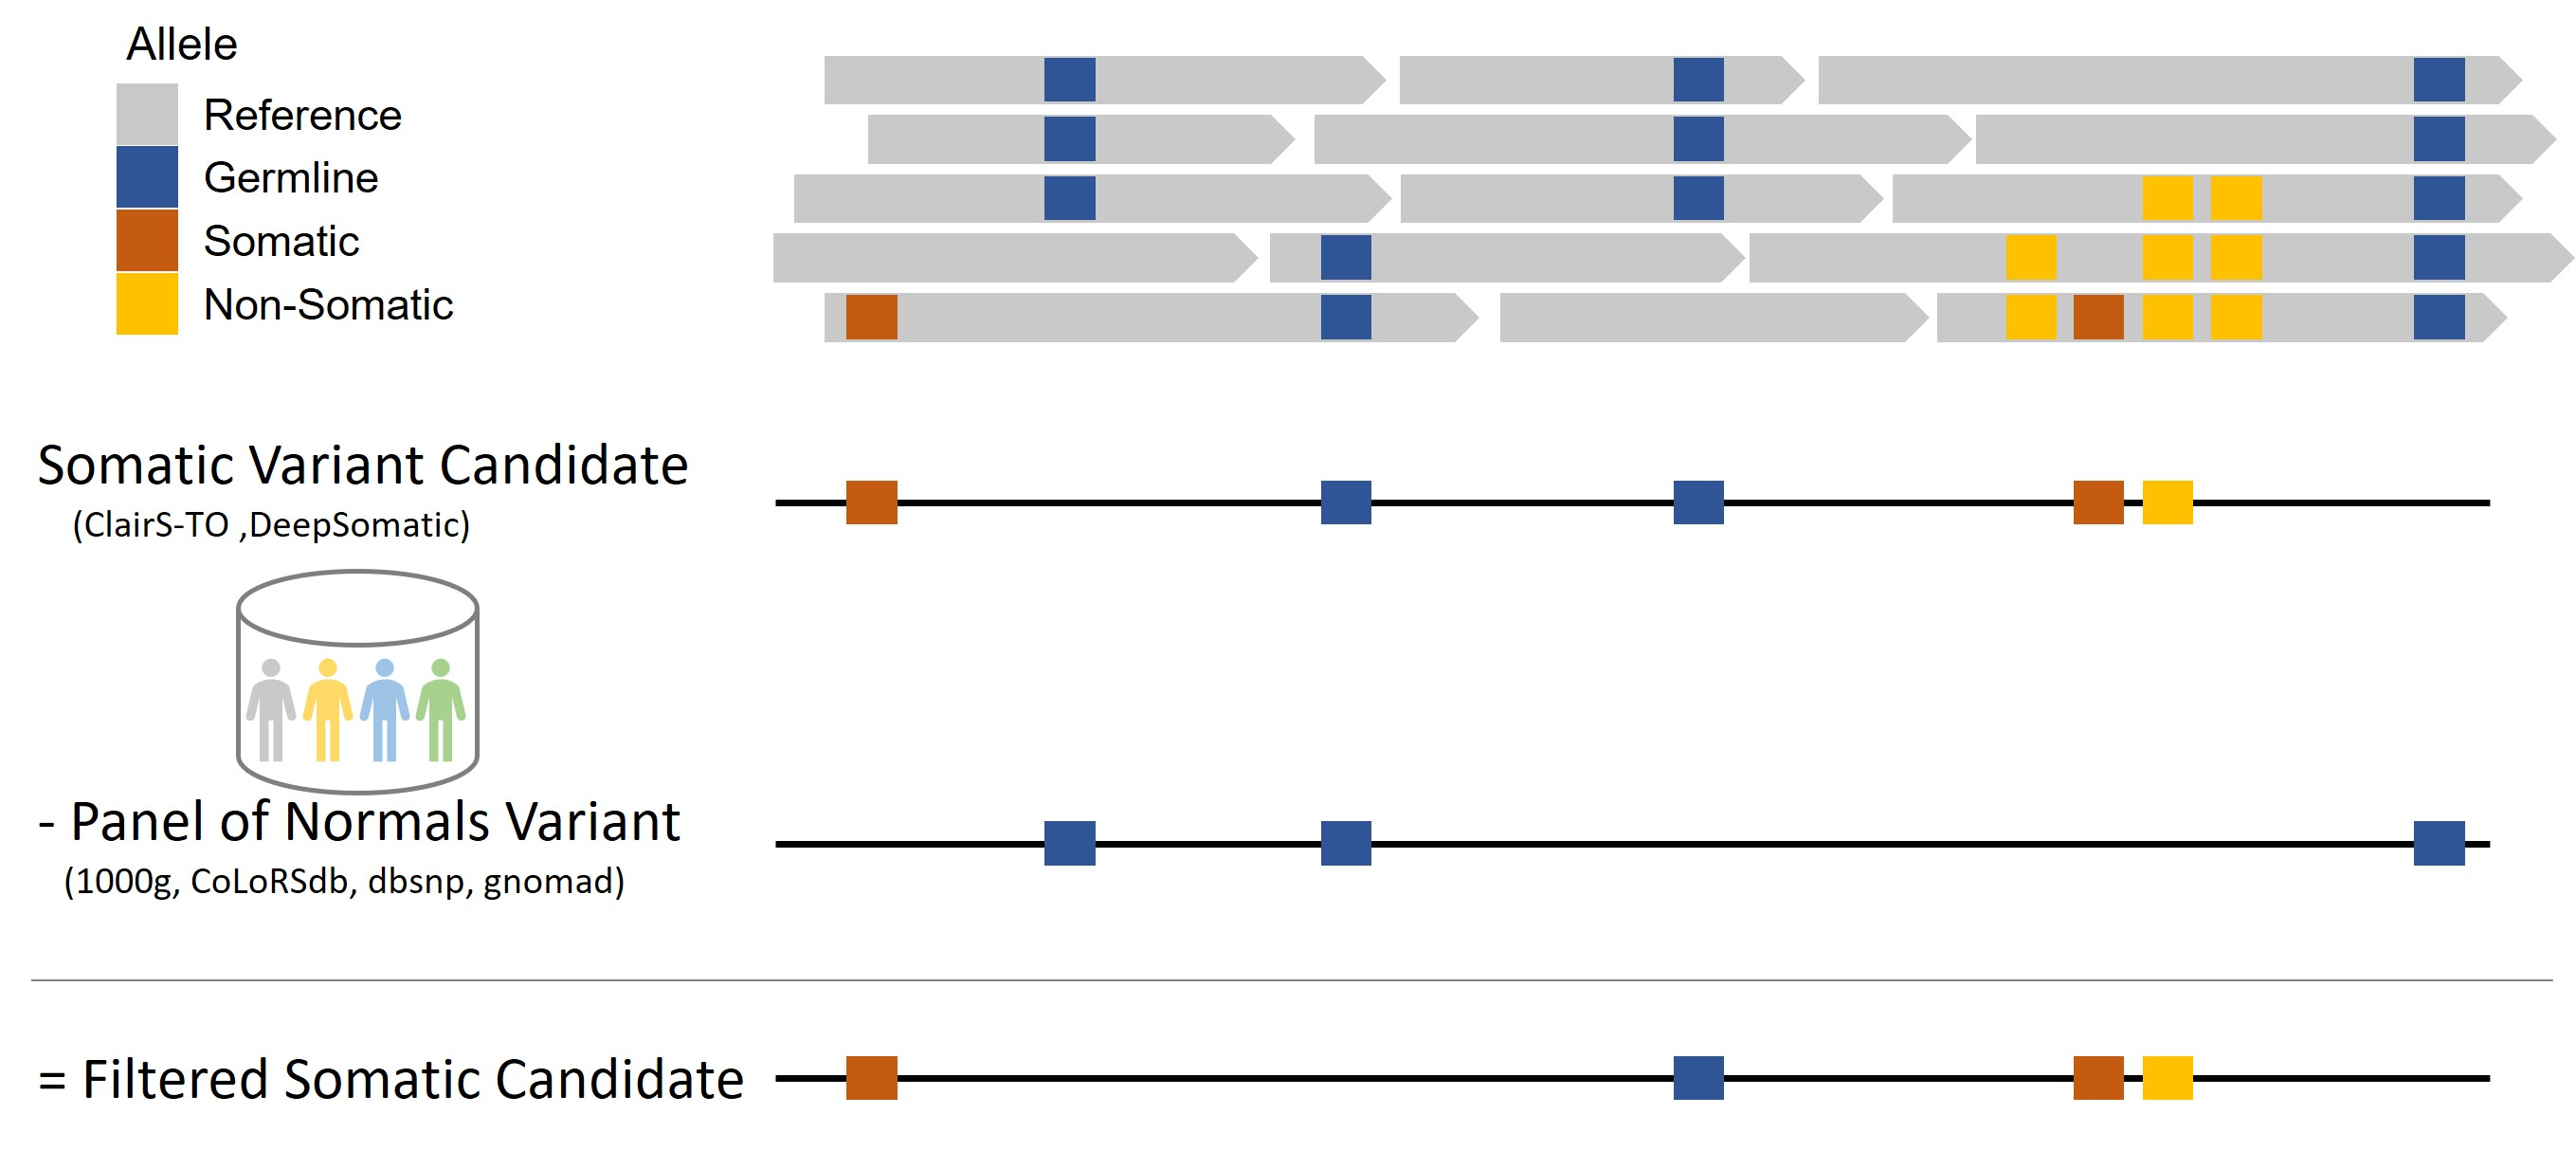
\includegraphics[width=0.8\textwidth,keepaspectratio]{page_18_cropped.jpg}}
\caption[Panel of Normals Filtering]{Filtering somatic variant candidates using a Panel of Normals (PON). This schematic shows that an initial set of variant candidates, containing a mix of somatic (brown), germline (blue), and other variants, is filtered by subtracting all variants found in the PON. This process enriches the final candidate list for true somatic mutations by removing common germline polymorphisms and known artifacts.}\label{fig:met-page-18-cropped-jpg}
\end{figure}

\paragraph{Filtering of Clustered Variants via Allele Concordance}\label{filtering-of-clustered-variants-via-allele-concordance}

Systematic sequencing and alignment errors often manifest as clusters of false positive variants in close proximity. To identify and remove these artifacts, an Allele Concordance filter is employed. This method evaluates a candidate variant at position $i$ by analyzing its co-occurrence with neighboring variants on the same long reads. For a candidate variant $i$ and a nearby variant $j$, two concordance ratios are calculated:

\[
\frac{\text{AltAlt}_{ij}}{\text{AltAlt}_{ij} + \text{AltRef}_{ij}} \ge \mu
\]

\[
\frac{\text{AltAlt}_{ij}}{\text{AltAlt}_{ij} + \text{RefAlt}_{ij}} \ge \nu
\]

where \(AltAlt_ij\) is the number of reads with alternate alleles at both \(i\) and \(j\), \(AltRef_ij\) is the count of reads with an alternate allele at \(i\) and reference at \(j\), and \(RefAlt_ij\) is the count of reads with reference at \(i\) and alternate at \(j\). The thresholds \(\mu\) and \(\nu\) control the stringency. If a candidate variant \(i\) shows high concordance with multiple neighbors (i.e., its aggregate Allele Concordance score exceeds a final threshold \(\rho\)), it is classified as a clustered artifact and removed from the candidate list (Figure~\ref{fig:met-page-19-cropped-jpg}).

\begin{figure}
\centering
\pandocbounded{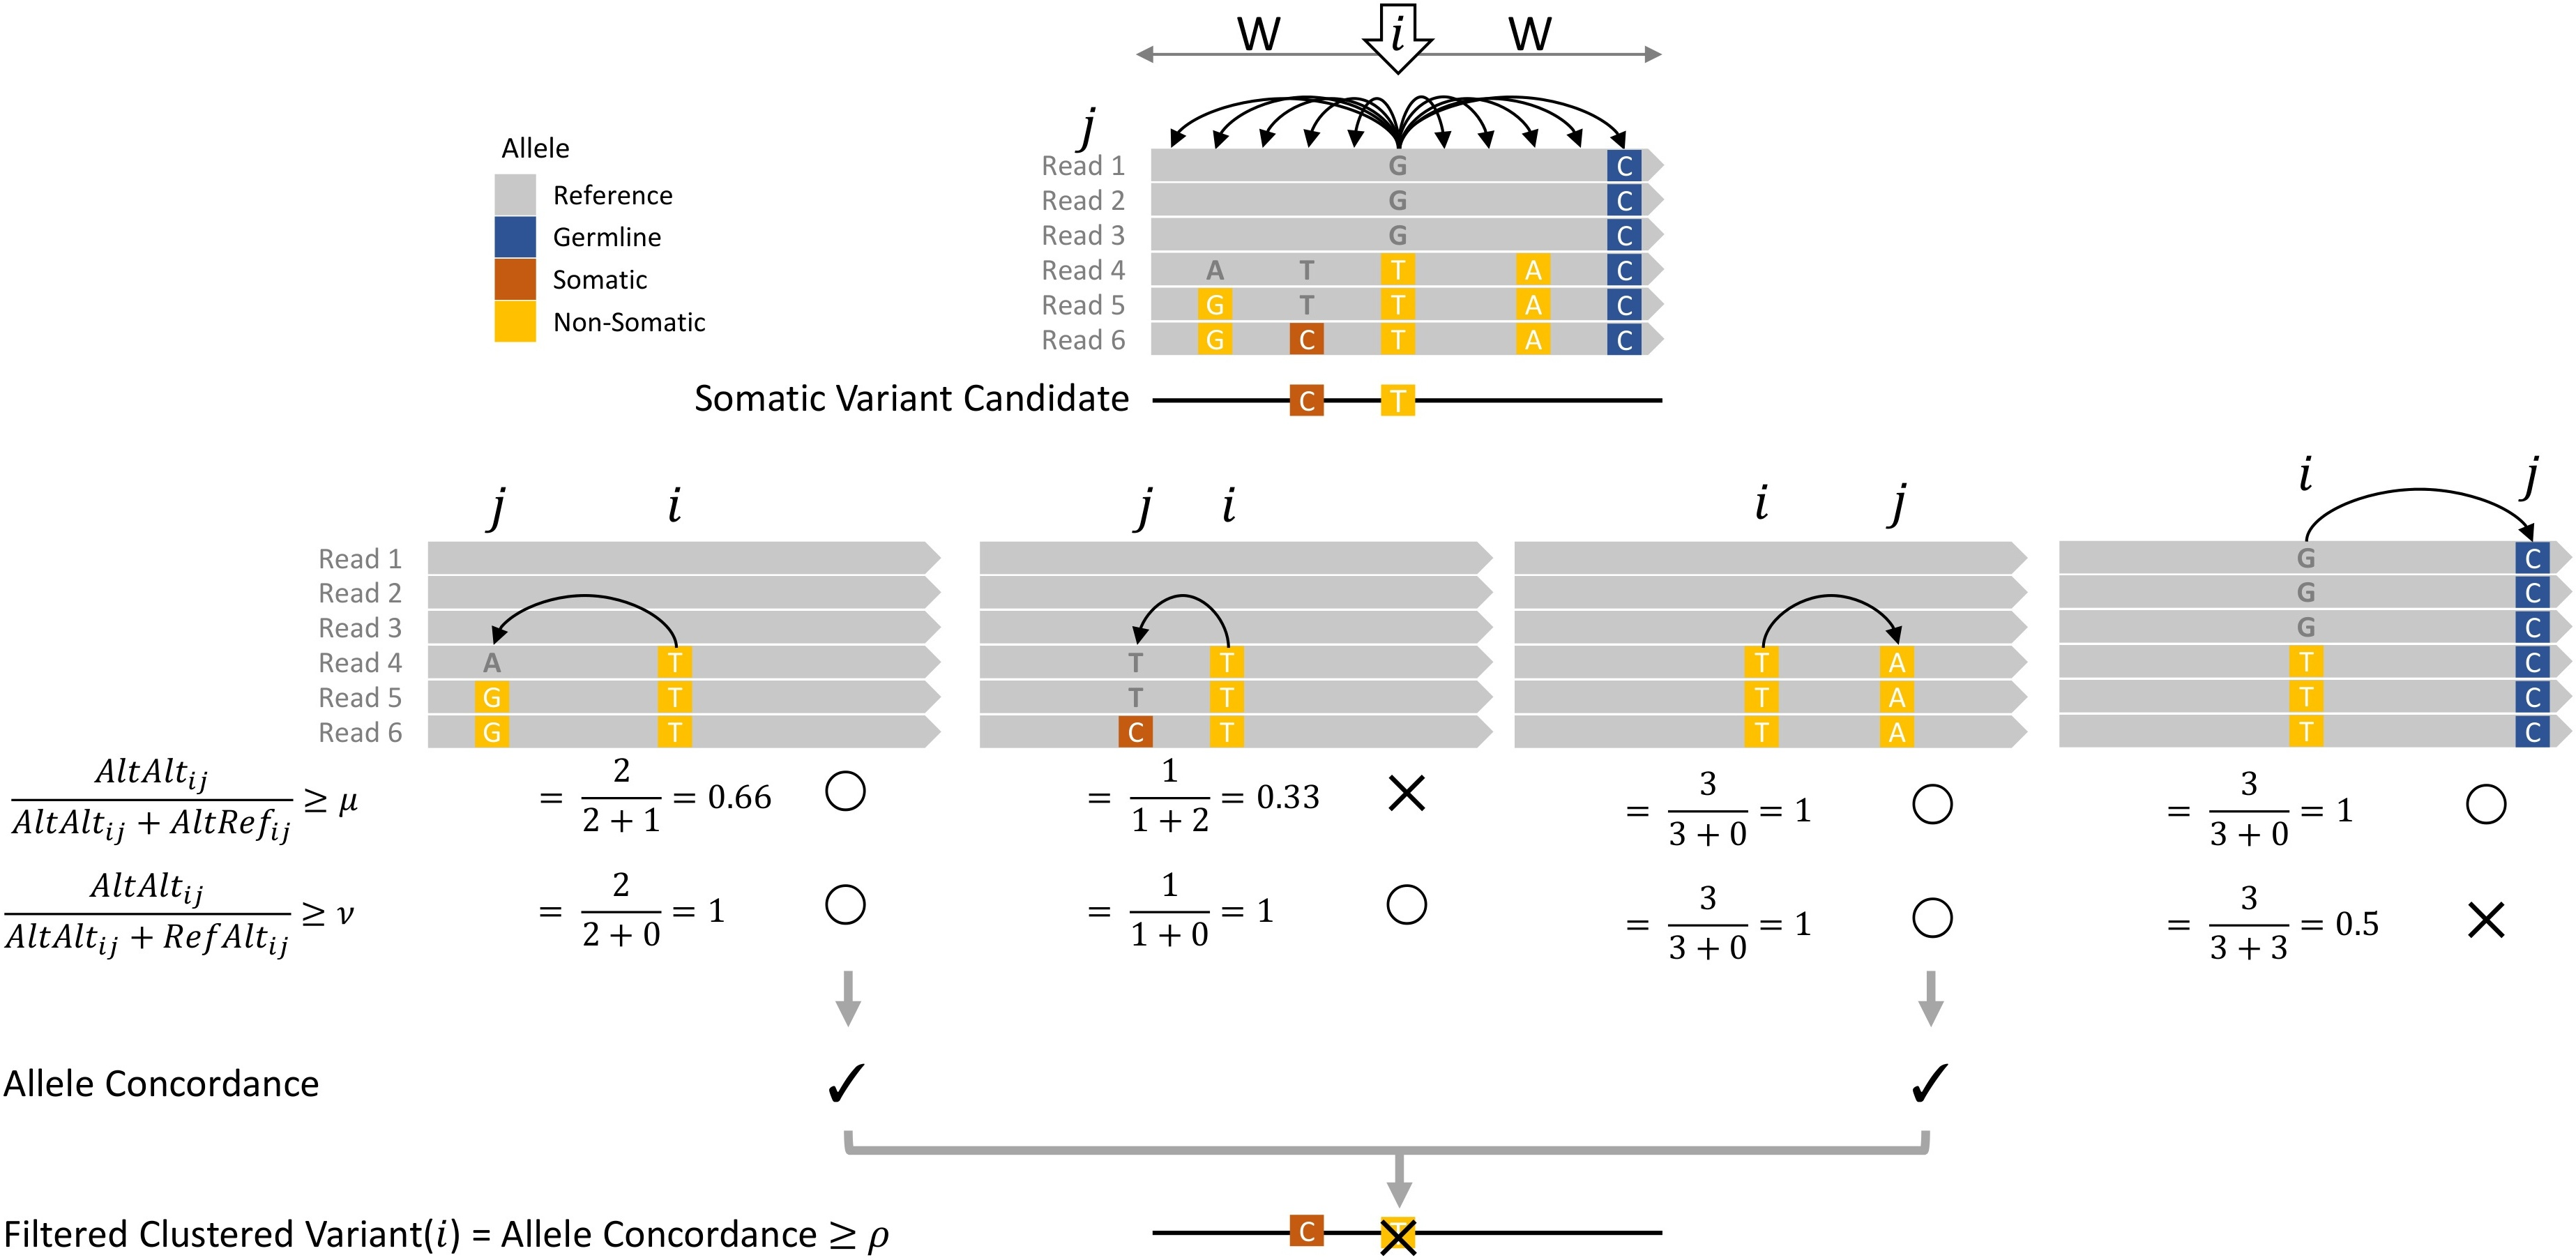
\includegraphics[keepaspectratio]{page_19_cropped.jpg}}
\caption[Allele Concordance Filtering]{Filtering of clustered artifacts using Allele Concordance. The method analyzes the co-occurrence of a candidate variant (at position \texttt{i}) with its neighbors (at position \texttt{j}) on the same long reads. Variants that consistently appear together (high concordance) are likely systematic artifacts. The workflow illustrates how pairs of variants are tested and, if the aggregate concordance score is high, the candidate is filtered out.}\label{fig:met-page-19-cropped-jpg}
\end{figure}

\subsubsection{Graph-Based Somatic Variant Calling}\label{graph-based-somatic-variant-calling}

The filtered list of high-confidence candidates is then subjected to a novel, graph-based variant calling algorithm designed to leverage local haplotype information.

\paragraph{The Tri-nodal-edge Graph Model}\label{the-tri-nodal-edge-graph-model}

Since somatic variants arise post-zygotically and humans are diploid, each somatic mutation must originate from one of the existing haplotypes and subsequently diverge from it. In contrast, sequencing artifacts are expected to occur randomly and therefore lack such haplotype-specific origins. Based on this principle, the Tri-nodal-edge Graph, a data structure designed to model allele linkages across three adjacent variant positions, enabling discrimination between true somatic mutations and sequencing artifacts. Compared with the simpler Bi-nodal-edge Graph, which only considers variant pairs and can be found to be insufficient for resolving complex cases, the Tri-nodal-edge Graph captures a richer local haplotype context. In this representation, nodes correspond to alleles (reference or alternate), while weighted edges encode the observed three-variant haplotypes together with their supporting read counts (Figure~\ref{fig:met-page-20-cropped-jpg}).

\begin{figure}
\centering
\pandocbounded{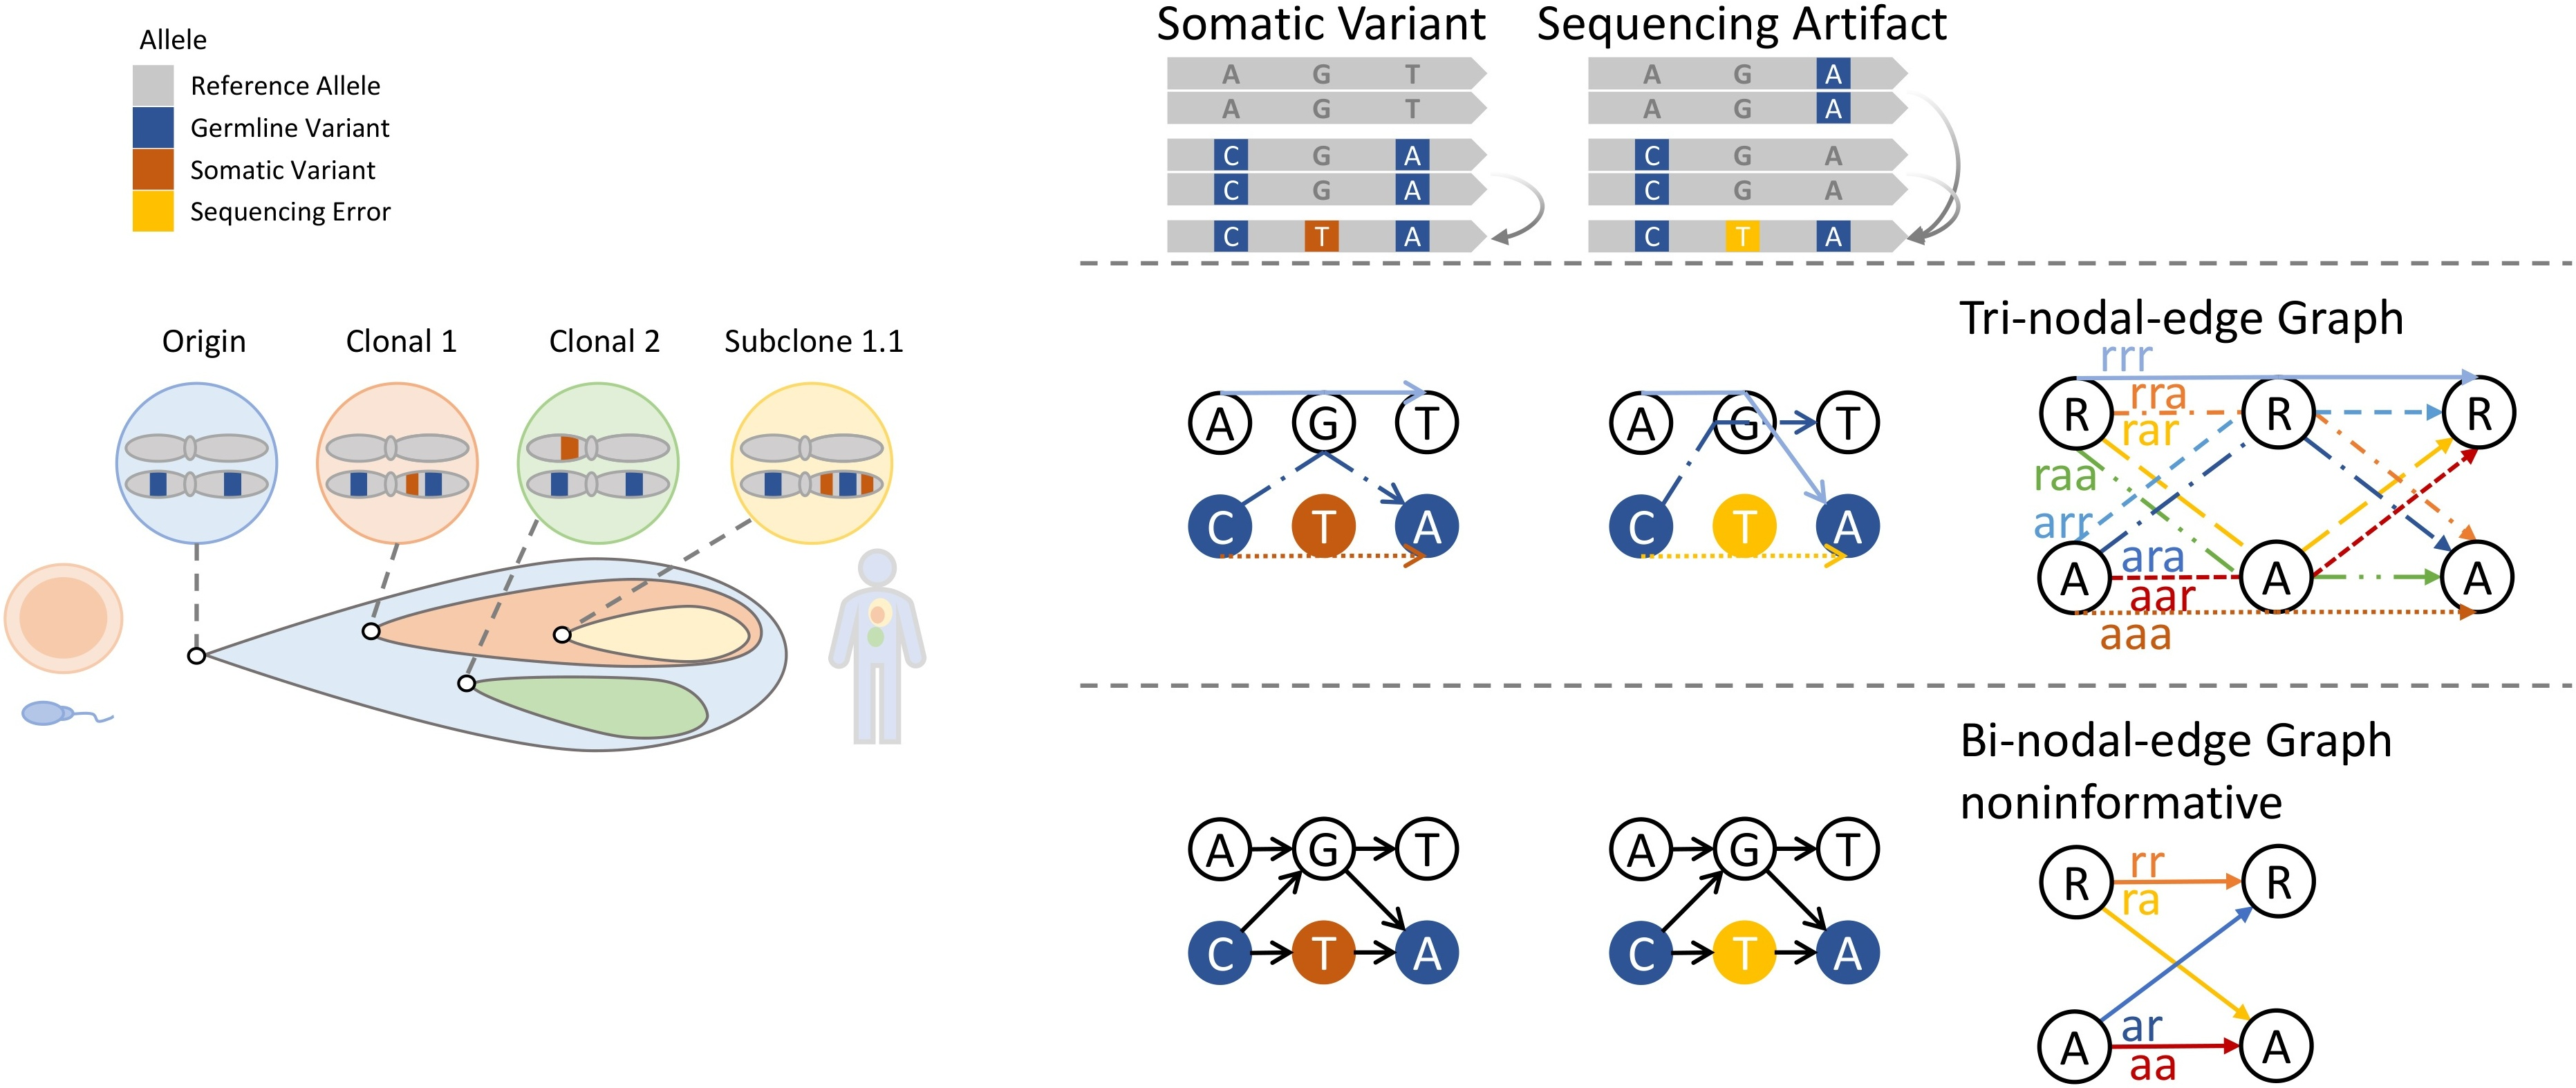
\includegraphics[keepaspectratio]{page_20_cropped.jpg}}
\caption[Graph Models Comparison]{Comparison of graph models for somatic variant calling. The figure contrasts the proposed Tri-nodal-edge Graph, which models haplotypes across three adjacent variant sites, with a simpler Bi-nodal-edge Graph that only considers pairs. The Tri-nodal-edge graph captures more linkage information, making it more powerful for distinguishing true somatic variants from artifacts, while the Bi-nodal-edge graph is labeled noninformative for this complex task.}\label{fig:met-page-20-cropped-jpg}
\end{figure}

\paragraph{Combinatorial Haplotype Pattern Classification}\label{combinatorial-haplotype-pattern-classification}

A variant is classified not in isolation, but by matching the combination of local haplotypes observed at its locus against a predefined catalog of patterns (Figure~\ref{fig:met-page-21-cropped-jpg}). These patterns fall into three categories:

\begin{itemize}
\tightlist
\item
  \textbf{High-Confidence Somatic \(V_H\):} These patterns arise from a 3-haplotype scenario, in which the paternal and maternal germline haplotypes are distinct, and an additional somatic haplotype emerges. In other words, the sequencing reads support two germline haplotypes and one somatic haplotype. Among all \(C(8,3) = 56\) possible 3-haplotype combinations, the study identifies 12 specific evolutionary configurations that are classified as High-Confidence Somatic \(V_H\) patterns.
\item
  \textbf{Low-Confidence Somatic \(V_L\):} These patterns arise from simpler 2-haplotype scenarios, in which the paternal and maternal germline haplotypes are identical, and an additional somatic haplotype emerges. In other words, the sequencing reads support one germline haplotype and one somatic haplotype. Among all \(C(8,2) = 28\) possible 2-haplotype combinations, the study identifies 3 specific configurations that are classified as Low-Confidence Somatic \(V_L\) patterns.
\item
  \textbf{Non-Somatic \(V_N\):} Any observed haplotype combination not matching a \(V_H\) or \(V_L\) pattern.
\end{itemize}

\begin{figure}
\centering
\pandocbounded{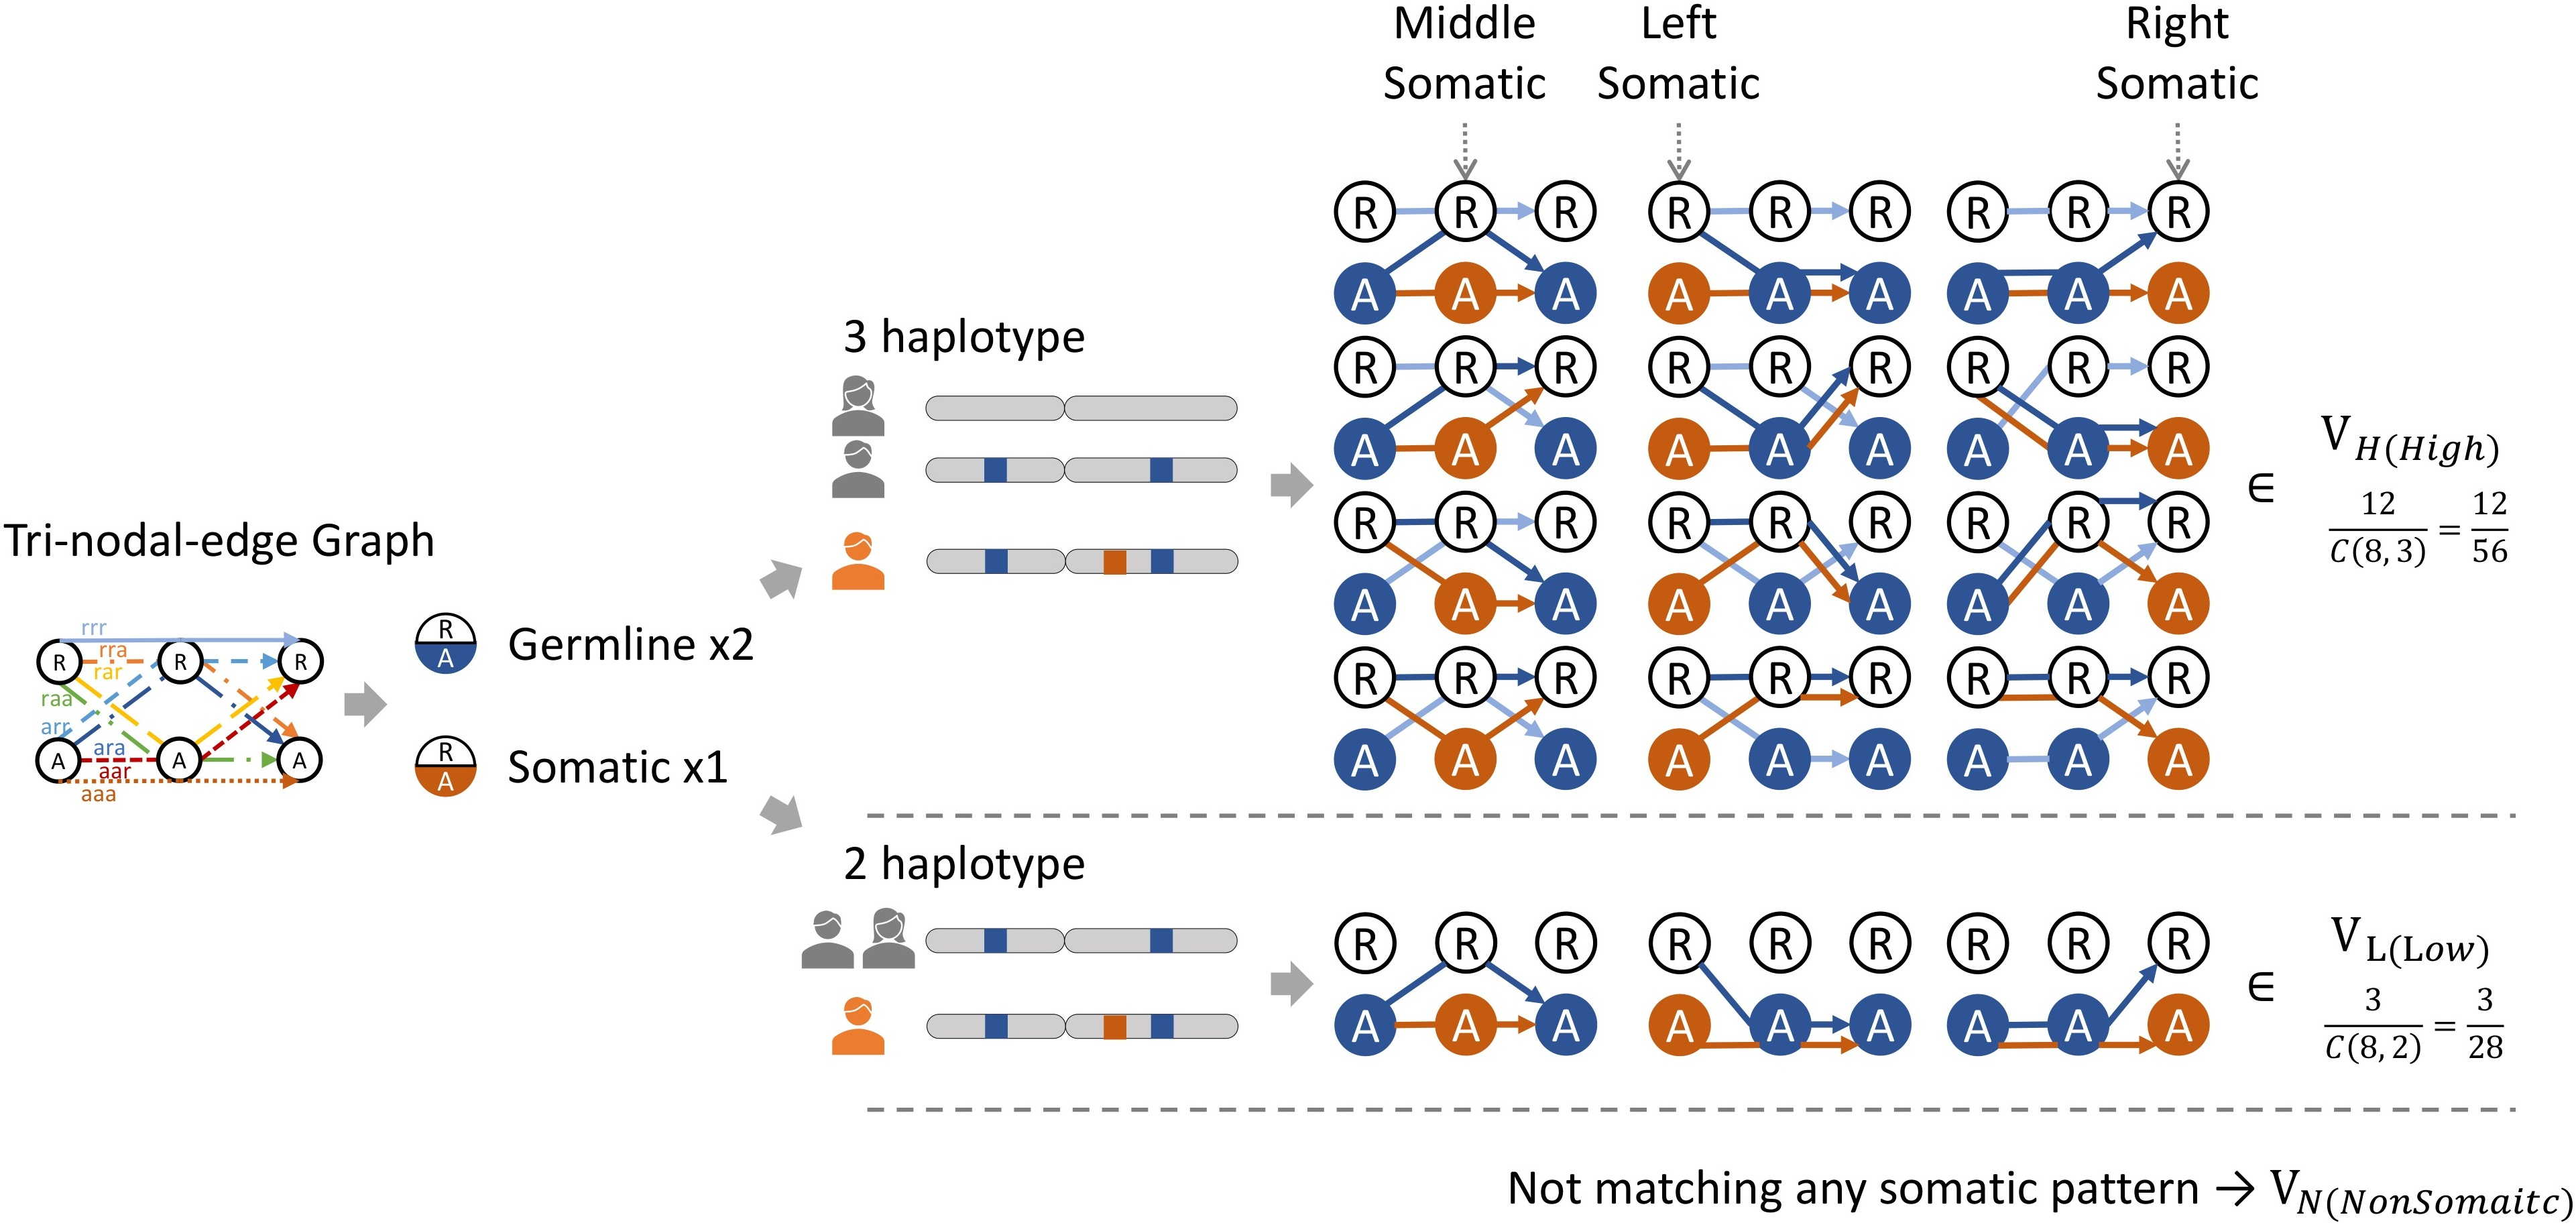
\includegraphics[keepaspectratio]{page_21_cropped.jpg}}
\caption[Combinatorial Haplotype Pattern Classification]{High-confidence patterns ($V_H$) arise from three-haplotype scenarios with two distinct germline haplotypes and one somatic haplotype, while low-confidence patterns ($V_L$) arise from two-haplotype scenarios with identical germline haplotypes and one somatic haplotype. All other combinations are classified as non-somatic ($V_N$).}\label{fig:met-page-21-cropped-jpg}
\end{figure}

\paragraph{Pattern Mining and Artifact Filtering}\label{pattern-mining-and-artifact-filtering}

In practical applications, the haplotype graph often contains more than three possible paths between alleles. To determine whether a candidate variant conforms to a $V_H$ (High-Confidence Somatic) pattern, all possible paths (up to eight in total) by their supporting read counts and select the top three for evaluation. This top-3 selection increases sensitivity but also introduces the possibility of ties in path frequencies. Consequently, a candidate variant may simultaneously match both $V_H$ and $V_N$ (Non-Somatic) pattern criteria.

To address such ambiguity, an artifact path ratio metric, which quantifies the proportion of sequencing noise within the top-3 paths that match the $V_H$ pattern definition. Specifically, if the artifact path ratio exceeds a predefined threshold $\tau$, the variant is reclassified from $V_H$ to $V_N$, thereby mitigating false-positive somatic calls due to sequencing artifacts.

A similar strategy is applied for $V_L$ (Low-Confidence Somatic) pattern detection. In this case, only the top two most frequent paths are selected for evaluation. As with $V_H$, ties in path frequencies can lead to ambiguous classification between $V_L$ and $V_N$. To resolve this, the relative artifact proportion between the top-3 and top-2 path sets. If the noise contribution within the $V_L$ pattern exceeds a separate threshold $\delta$, the candidate is downgraded to $V_N$ (Figure~\ref{fig:met-page-22-cropped-jpg}).

This two-tiered filtering approach—frequency-based path selection followed by artifact-based reclassification—ensures that both $V_H$ and $V_L$ detections maintain high precision while retaining sensitivity in complex haplotype contexts.

\begin{figure}
\centering
\pandocbounded{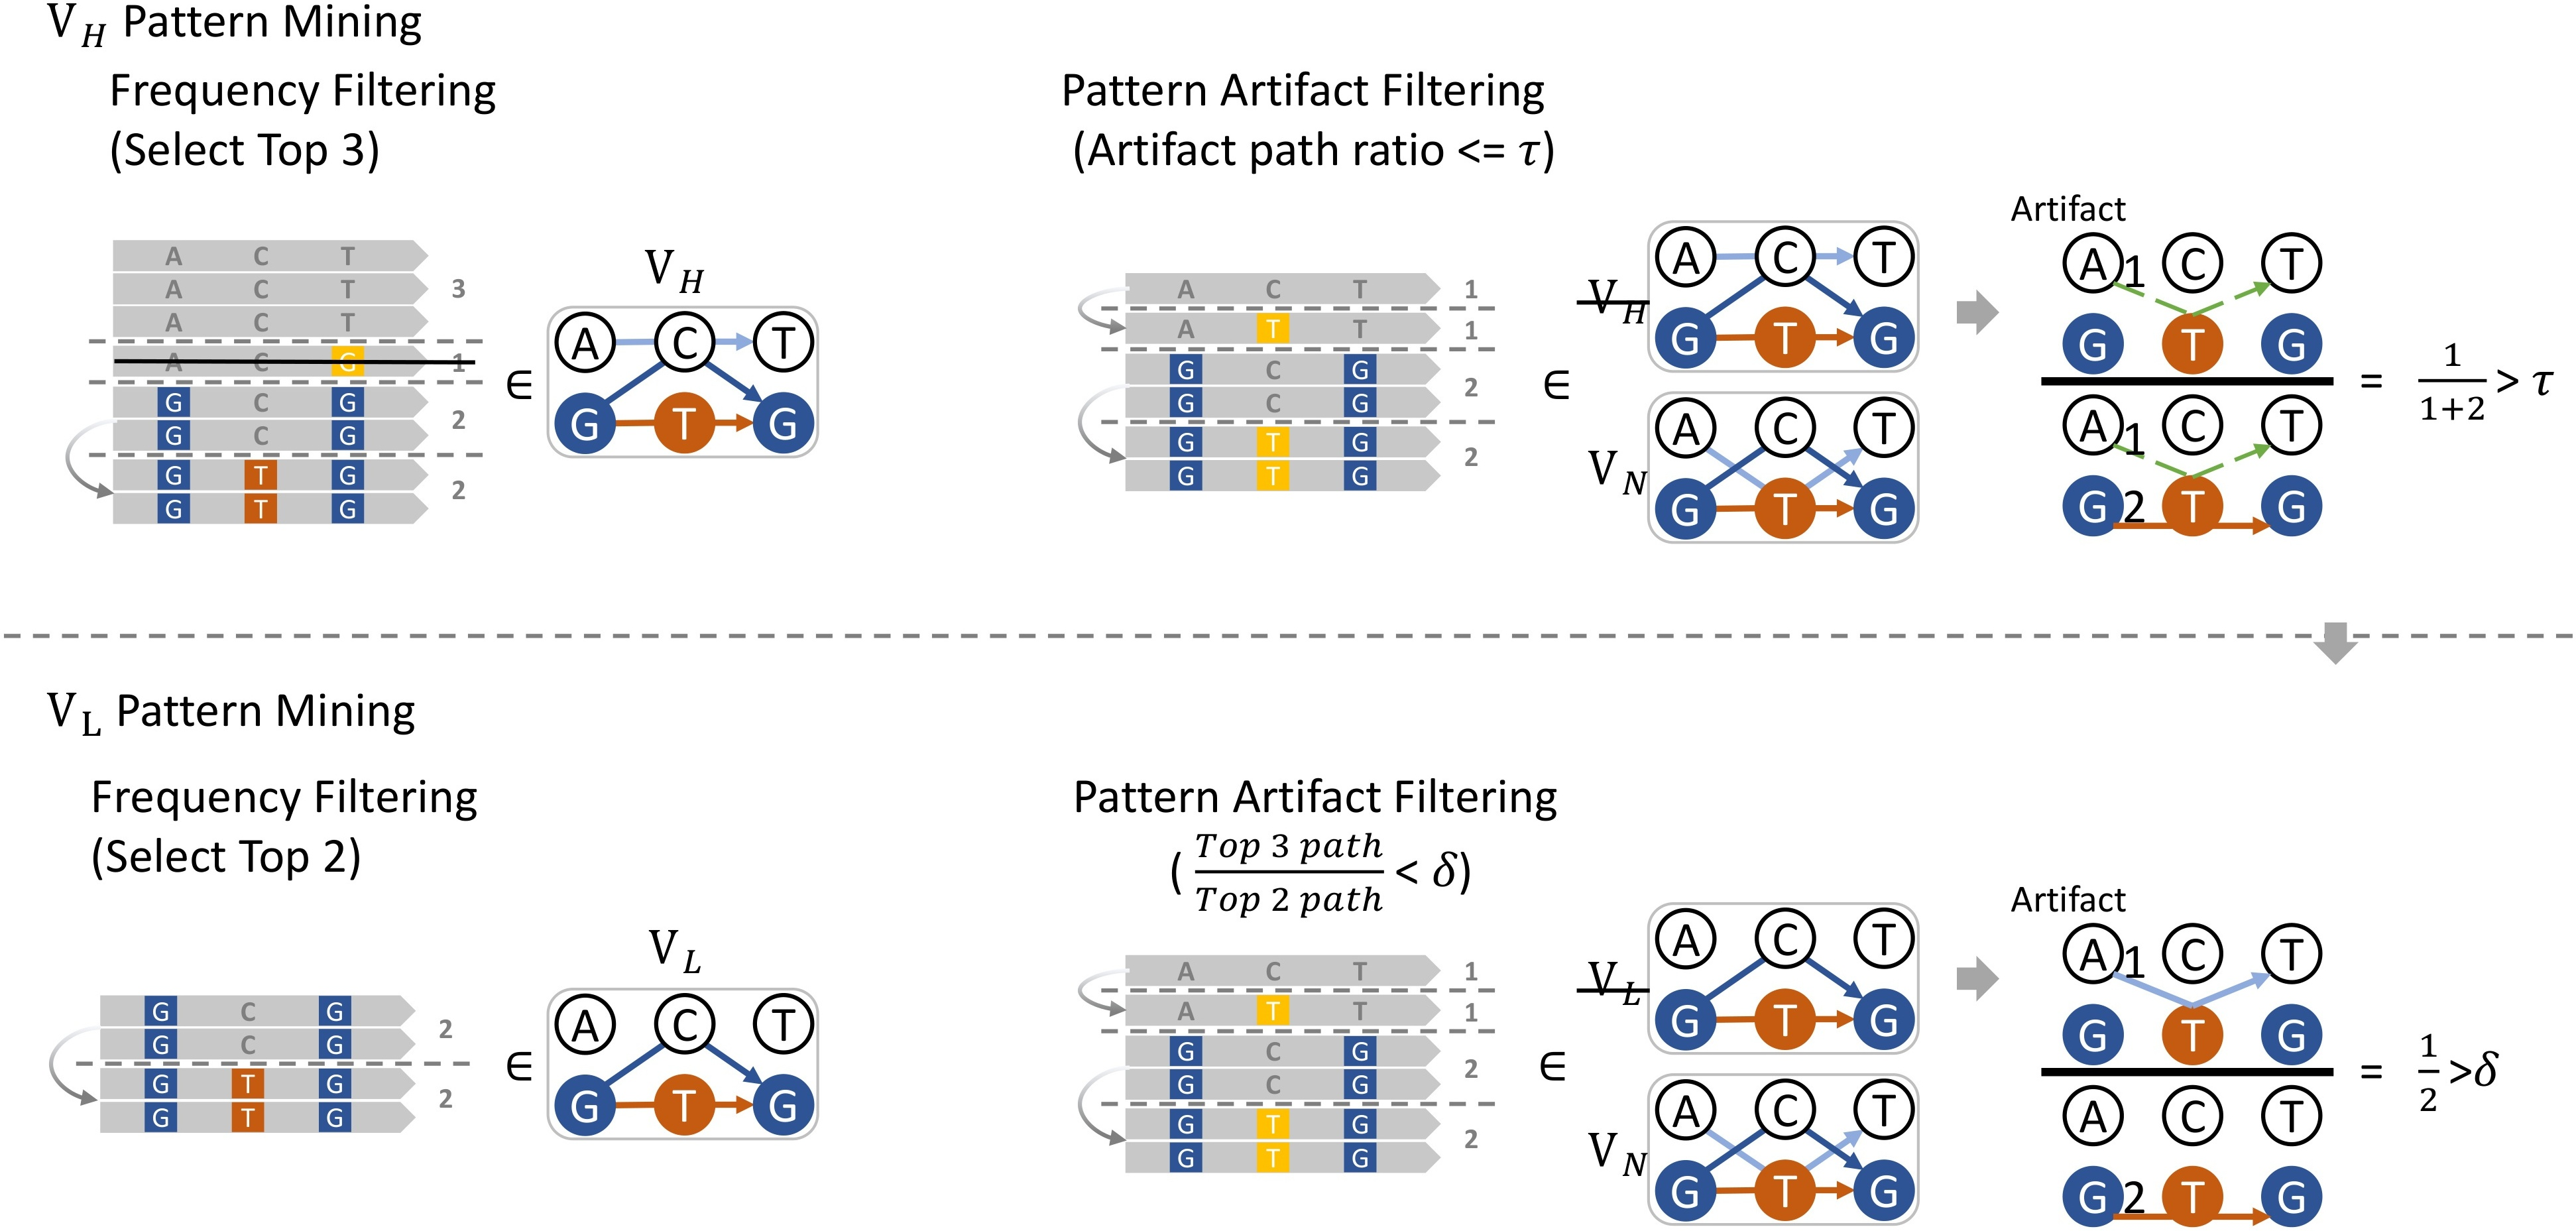
\includegraphics[keepaspectratio]{page_22_cropped.jpg}}
\caption[Artifact Filtering]{Filtering strategy for $V_H$ and $V_L$ haplotype patterns. Top-ranked haplotype paths are first selected by read support, followed by artifact-based reclassification. Variants exceeding the noise thresholds ($\tau$ for $V_H$, $\delta$ for $V_L$) are reassigned as $V_N$, ensuring accurate somatic variant detection in complex haplotype contexts.}\label{fig:met-page-22-cropped-jpg}
\end{figure}

\paragraph{Final Somatic Decision Formula}\label{final-somatic-decision-formula}

In practice, the decision for a candidate variant is not made from a single local haplotype graph, but rather from the combined evidence of multiple graphs spanning a broader genomic context to capture richer haplotype linkage information. Specifically, for a site under evaluation, k variants (where k denotes the number of variant sites) to both the upstream and downstream directions, resulting in a total span of 2k bases around the focal point. Within this window, overlapping subgraphs are constructed, such that each local graph covers the central site and the k surrounding positions on either side. This process yields \(k^2\) distinct Tri-nodal-edge graphs on each side of the focal site, with possible overlap between the left and right contexts. Consequently, a total of \(3k^2\) local graphs contribute to the classification decision for a single site.

The final somatic determination is made using a voting-based aggregation system, which integrates the evidence from all local haplotype patterns (Figure~\ref{fig:met-page-23-cropped-jpg}). A site is classified as somatic if it satisfies either of the following conditions:

\begin{figure}
\centering
\pandocbounded{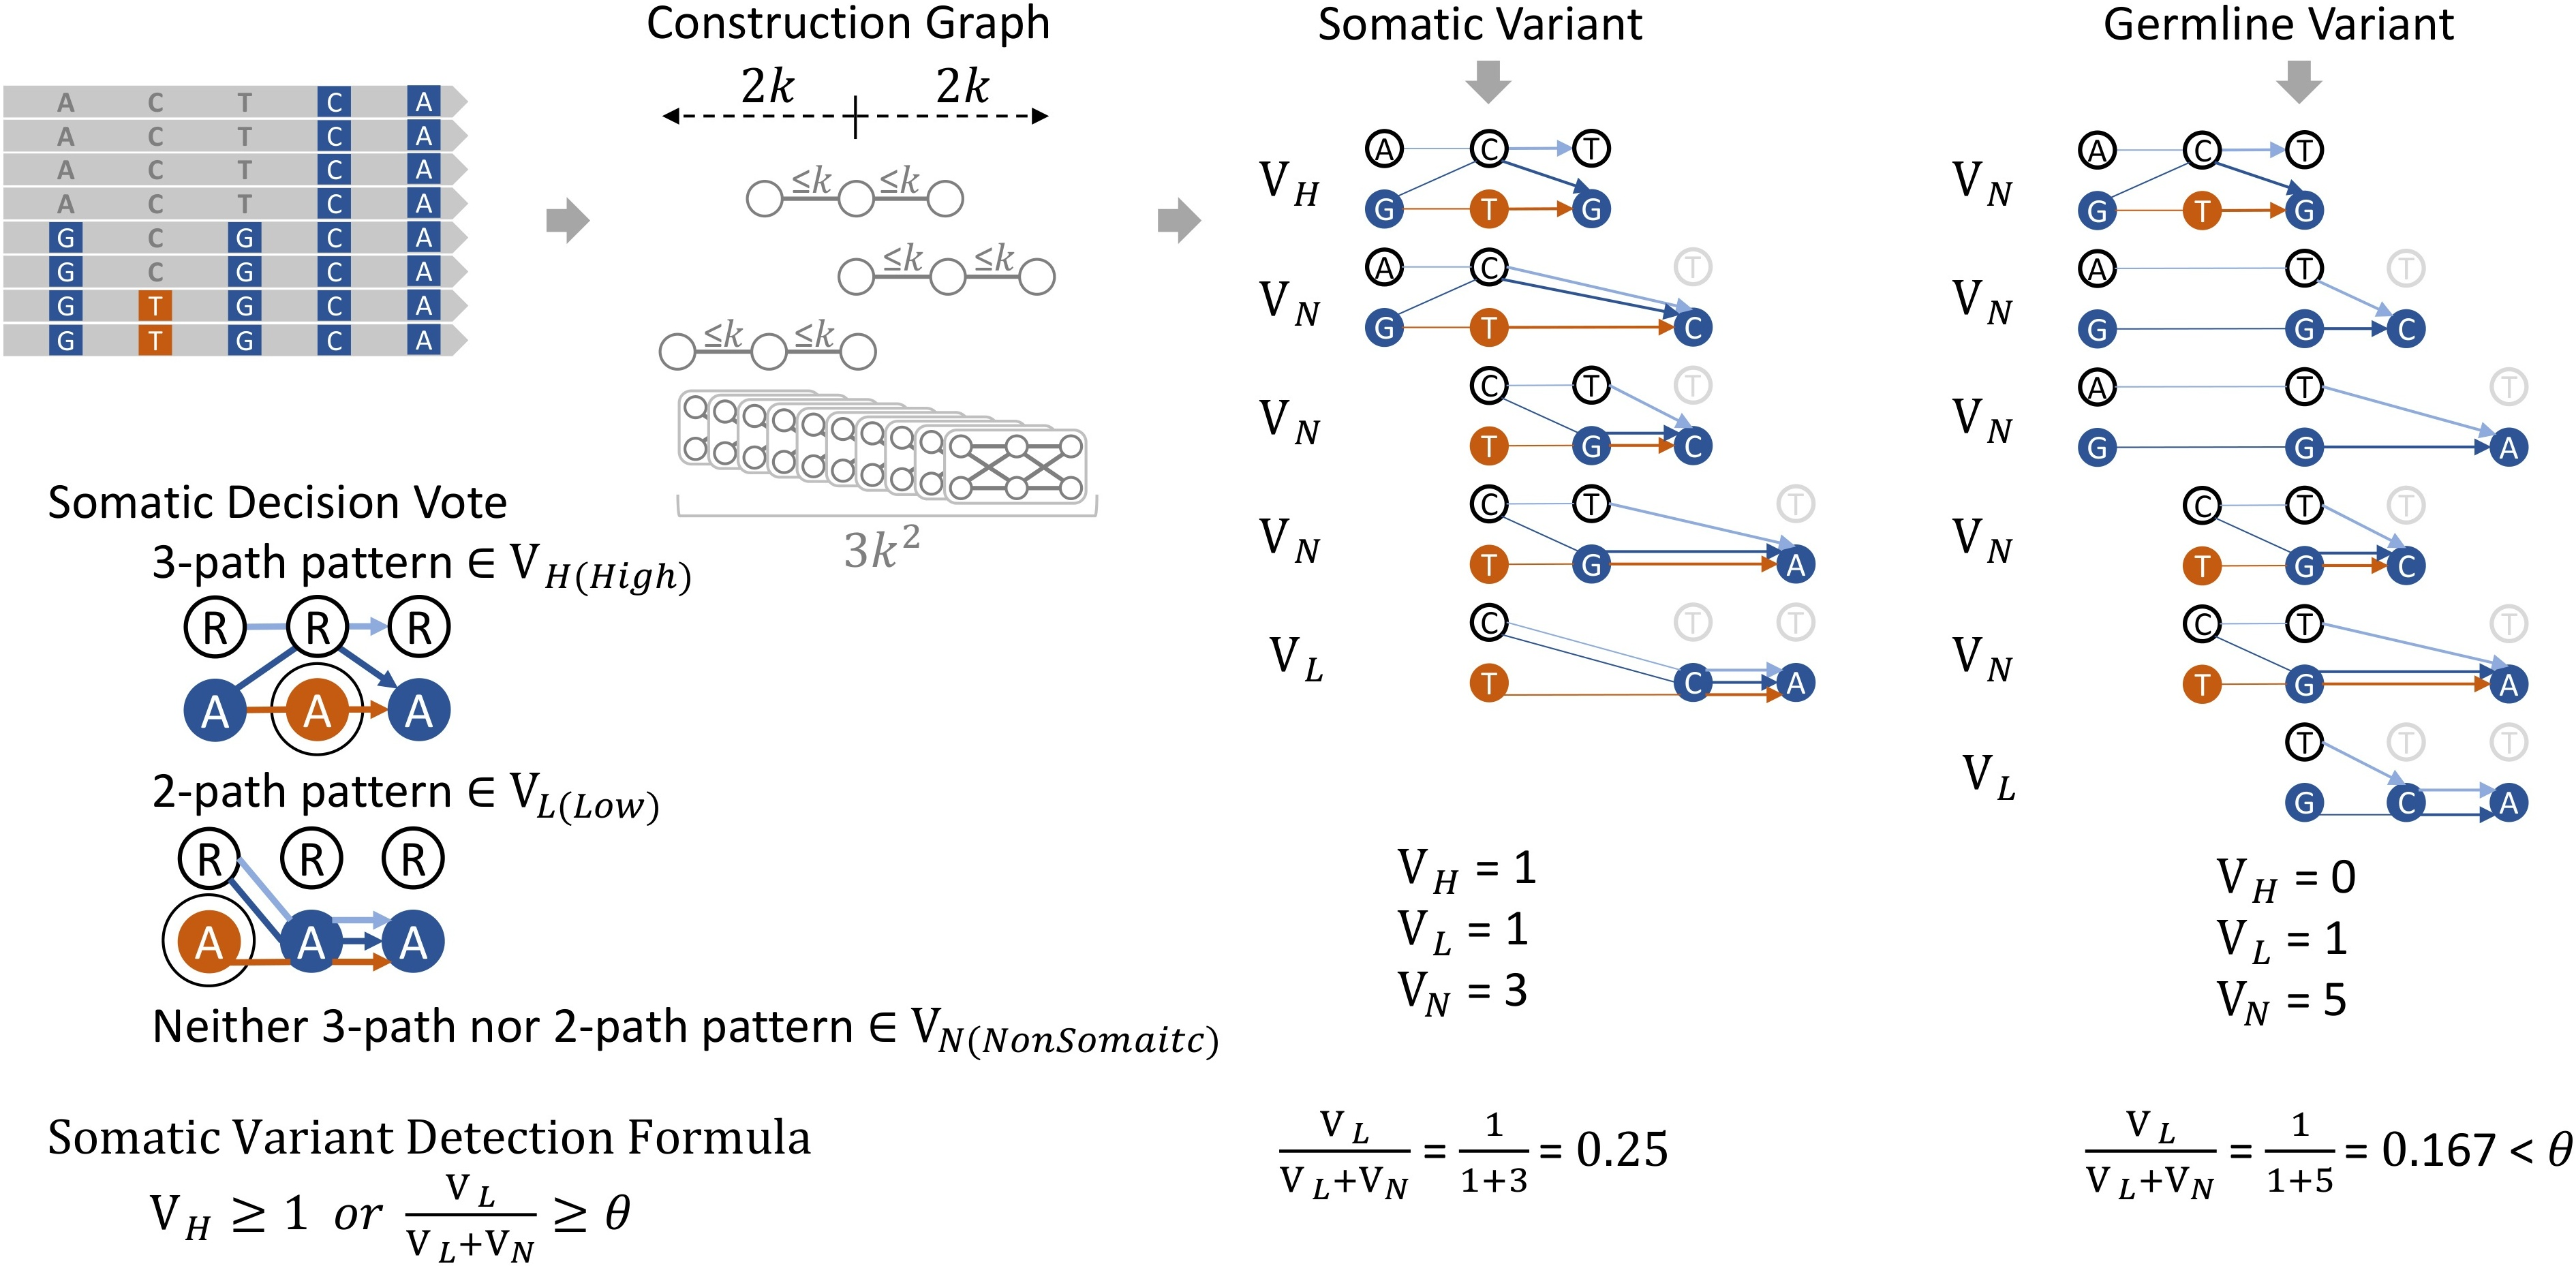
\includegraphics[keepaspectratio]{page_23_cropped.jpg}}
\caption[Final Decision Process]{The final decision-making process for somatic variant calling. This diagram illustrates how all local haplotype patterns at a site are classified as high-confidence \(V_H\), low-confidence \(V_L\), or non-somatic \(V_N\). These classifications are tallied in a voting system, and a final decision is made based on a formula that prioritizes \(V_H\) evidence or a significant proportion of \(V_L\) evidence.}\label{fig:met-page-23-cropped-jpg}
\end{figure}

\[
V_H \ge 1 \quad \text{or} \quad \frac{V_L}{V_L + V_N} \ge \theta
\]

This hierarchical rule ensures high sensitivity by calling any site with strong \(V_H\) evidence, while maintaining specificity by requiring weaker \(V_L\) evidence to surpass a statistical threshold $\theta$.

\subsubsection{Haplotype Phasing}\label{haplotype-phasing}

The foundation for the graph-based variant calling is a robust phasing
algorithm that reconstructs the full haplotypes present in the sample.

\paragraph{Graph-Based Haplotype Reconstruction}\label{graph-based-haplotype-reconstruction}

To resolve haplotype structures from sequencing data, we employed a graph-based reconstruction approach. A k-variant graph was first constructed, where each node represented an allele at a variant site and edges connected alleles observed on the same sequencing read (Figure~\ref{fig:met-page-24-cropped-jpg}). Edge weights corresponded to the number of supporting reads, thereby reflecting the strength of evidence for allele pairings. Haplotype reconstruction was initiated by designating the reference allele at the first variant site as haplotype 1 (HP1) and the corresponding alternative allele as haplotype 2 (HP2). These initial haplotype seeds were iteratively extended by traversing the graph in a left-to-right manner. At each step, possible allele combinations were evaluated, and the two non-overlapping paths that maximized consistency with observed read data were selected, yielding the most parsimonious haplotype reconstructions.

Building upon the variant calling results, which had already identified somatic mutations and detected regions of loss of heterozygosity (LOH), the k-variant graph further enabled systematic assignment of these events to their haplotype of origin. Somatic variants were phased by evaluating the sequencing reads that carried them, thereby establishing their linkage to specific germline haplotypes. Unlike conventional diploid phasing methods, this approach allowed the introduction of additional haplotype branches (e.g., HP2-1) to represent somatic haplotypes derived from distinct germline configurations. Within LOH regions, the graph structure was used to determine which haplotype paths were retained and which were lost, thereby clarifying haplotype loss. This integrative framework thus facilitated comprehensive phasing of both germline and somatic variants, including explicit resolution of LOH-associated haplotypes.

\begin{figure}
\centering
\pandocbounded{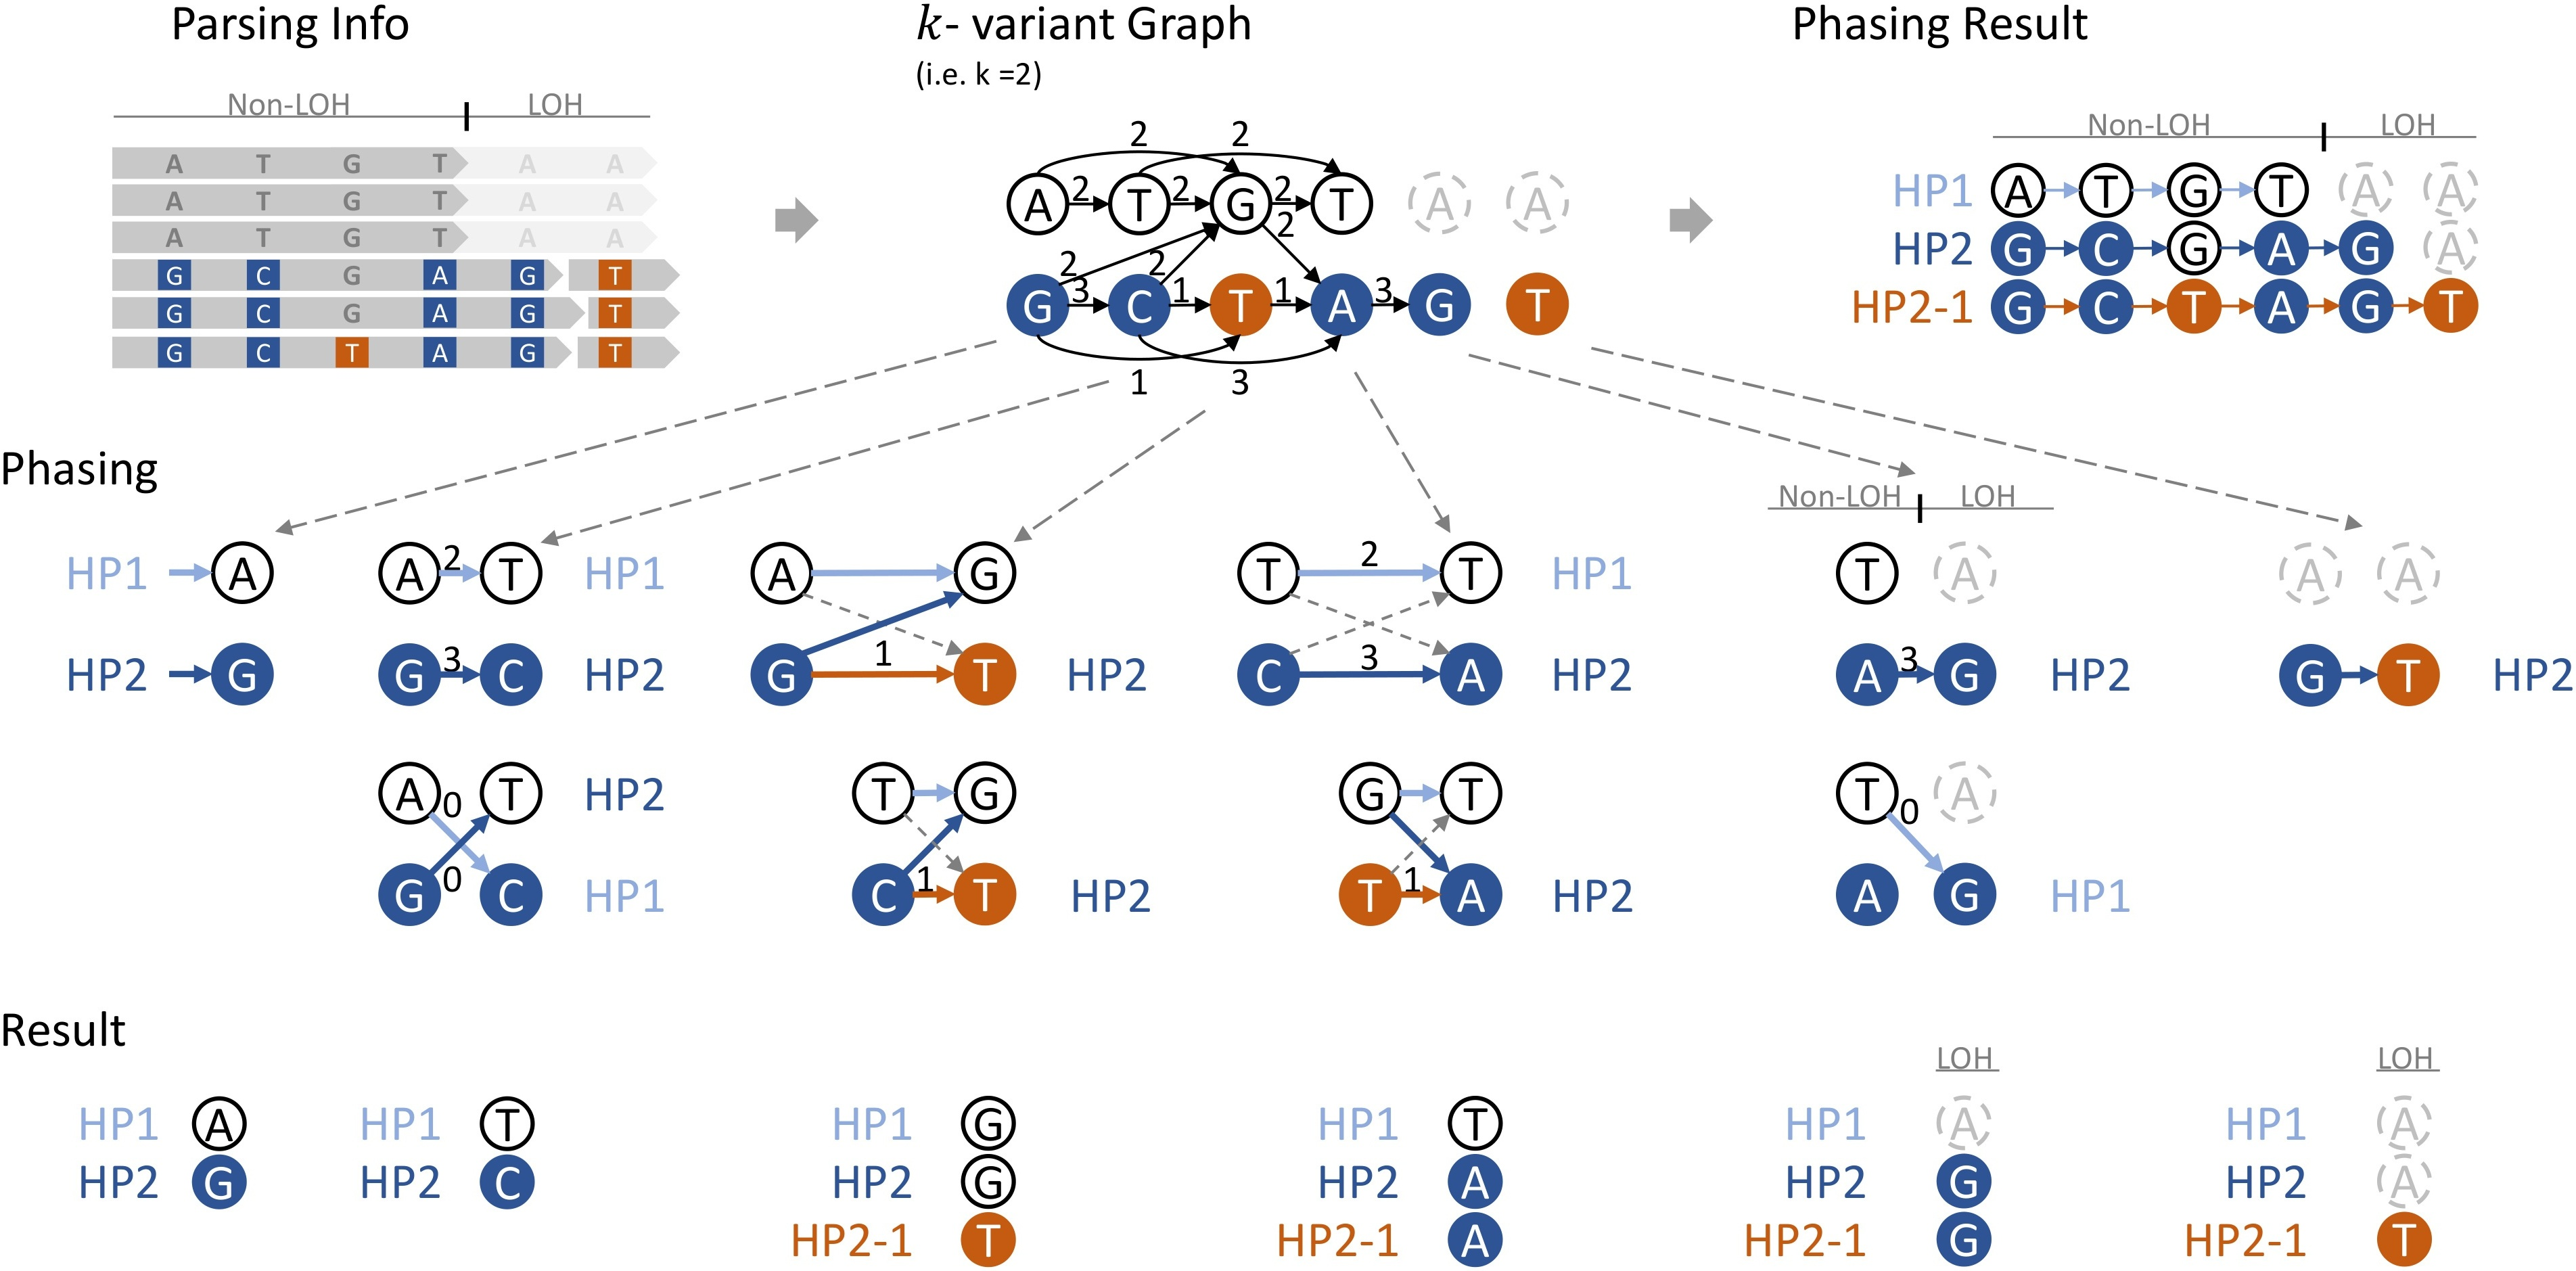
\includegraphics[keepaspectratio]{page_24_cropped.jpg}}
\caption[Haplotype Phasing Workflow]{Graph-based haplotype phasing workflow. This diagram illustrates how sequencing read data is transformed into a k-variant graph, where nodes are alleles and weighted edges represent their co-occurrence on reads. The algorithm then traverses this graph to reconstruct the most likely haplotypes, including distinguishing between germline (HP1, HP2) and newly evolved somatic (e.g., HP2-1) haplotypes.}\label{fig:met-page-24-cropped-jpg}
\end{figure}

\subsection{Tumor Purity Prediction}\label{tumor-purity-prediction}

Accurate estimation of tumor purity---the fraction of cancer cells in a sample---is essential for the correct interpretation of somatic variant data. Purity is predicted by modeling the genomic consequences of mixing tumor and normal cell populations.

\subsubsection{Principle of Haplotype Imbalance}\label{principle-of-haplotype-imbalance}

Information derived from haplotype imbalance (HI) can be further leveraged to estimate tumor purity. In practice, sequencing data often represent a mixture of tumor and normal cell populations. In a purely normal sample, the two germline haplotypes are expected to be equally represented, resulting in balanced HI values close to 0.5. As the fraction of tumor cells increases, this balance is progressively disrupted, and HI values shift away from 0.5 toward 1.0, reflecting increasing haplotype imbalance.

Formally, HI at each heterozygous site is defined as:
\[
\text{HI} = \frac{\max(\text{Count}_{\text{HP1}}, \text{Count}_{\text{HP2}})}{\text{Count}_{\text{HP1}} + \text{Count}_{\text{HP2}}}
\]

where $\text{Count}_{\text{HP1}}$ and $\text{Count}_{\text{HP2}}$ represent the allele-specific read counts assigned to the two germline haplotypes. To quantify the relationship between HI and tumor purity, HI is computed across all somatic variant sites and subsequently aggregated to capture the genome-wide distribution. Visualization using histograms or boxplots reveals a characteristic pattern: samples with low tumor purity exhibit HI values tightly centered around 0.5, whereas samples with high tumor purity display a systematic shift toward 1.0. This distributional change provides a quantitative basis for purity modeling. Accordingly, polynomial regression is applied to the observed HI distributions to establish a predictive relationship between HI and tumor purity. Once the regression model is trained, HI values derived from sequencing data can be directly input into the fitted function to yield accurate estimates of tumor purity (Figure~\ref{fig:met-page-25-cropped-jpg}).

\begin{figure}
\centering
\pandocbounded{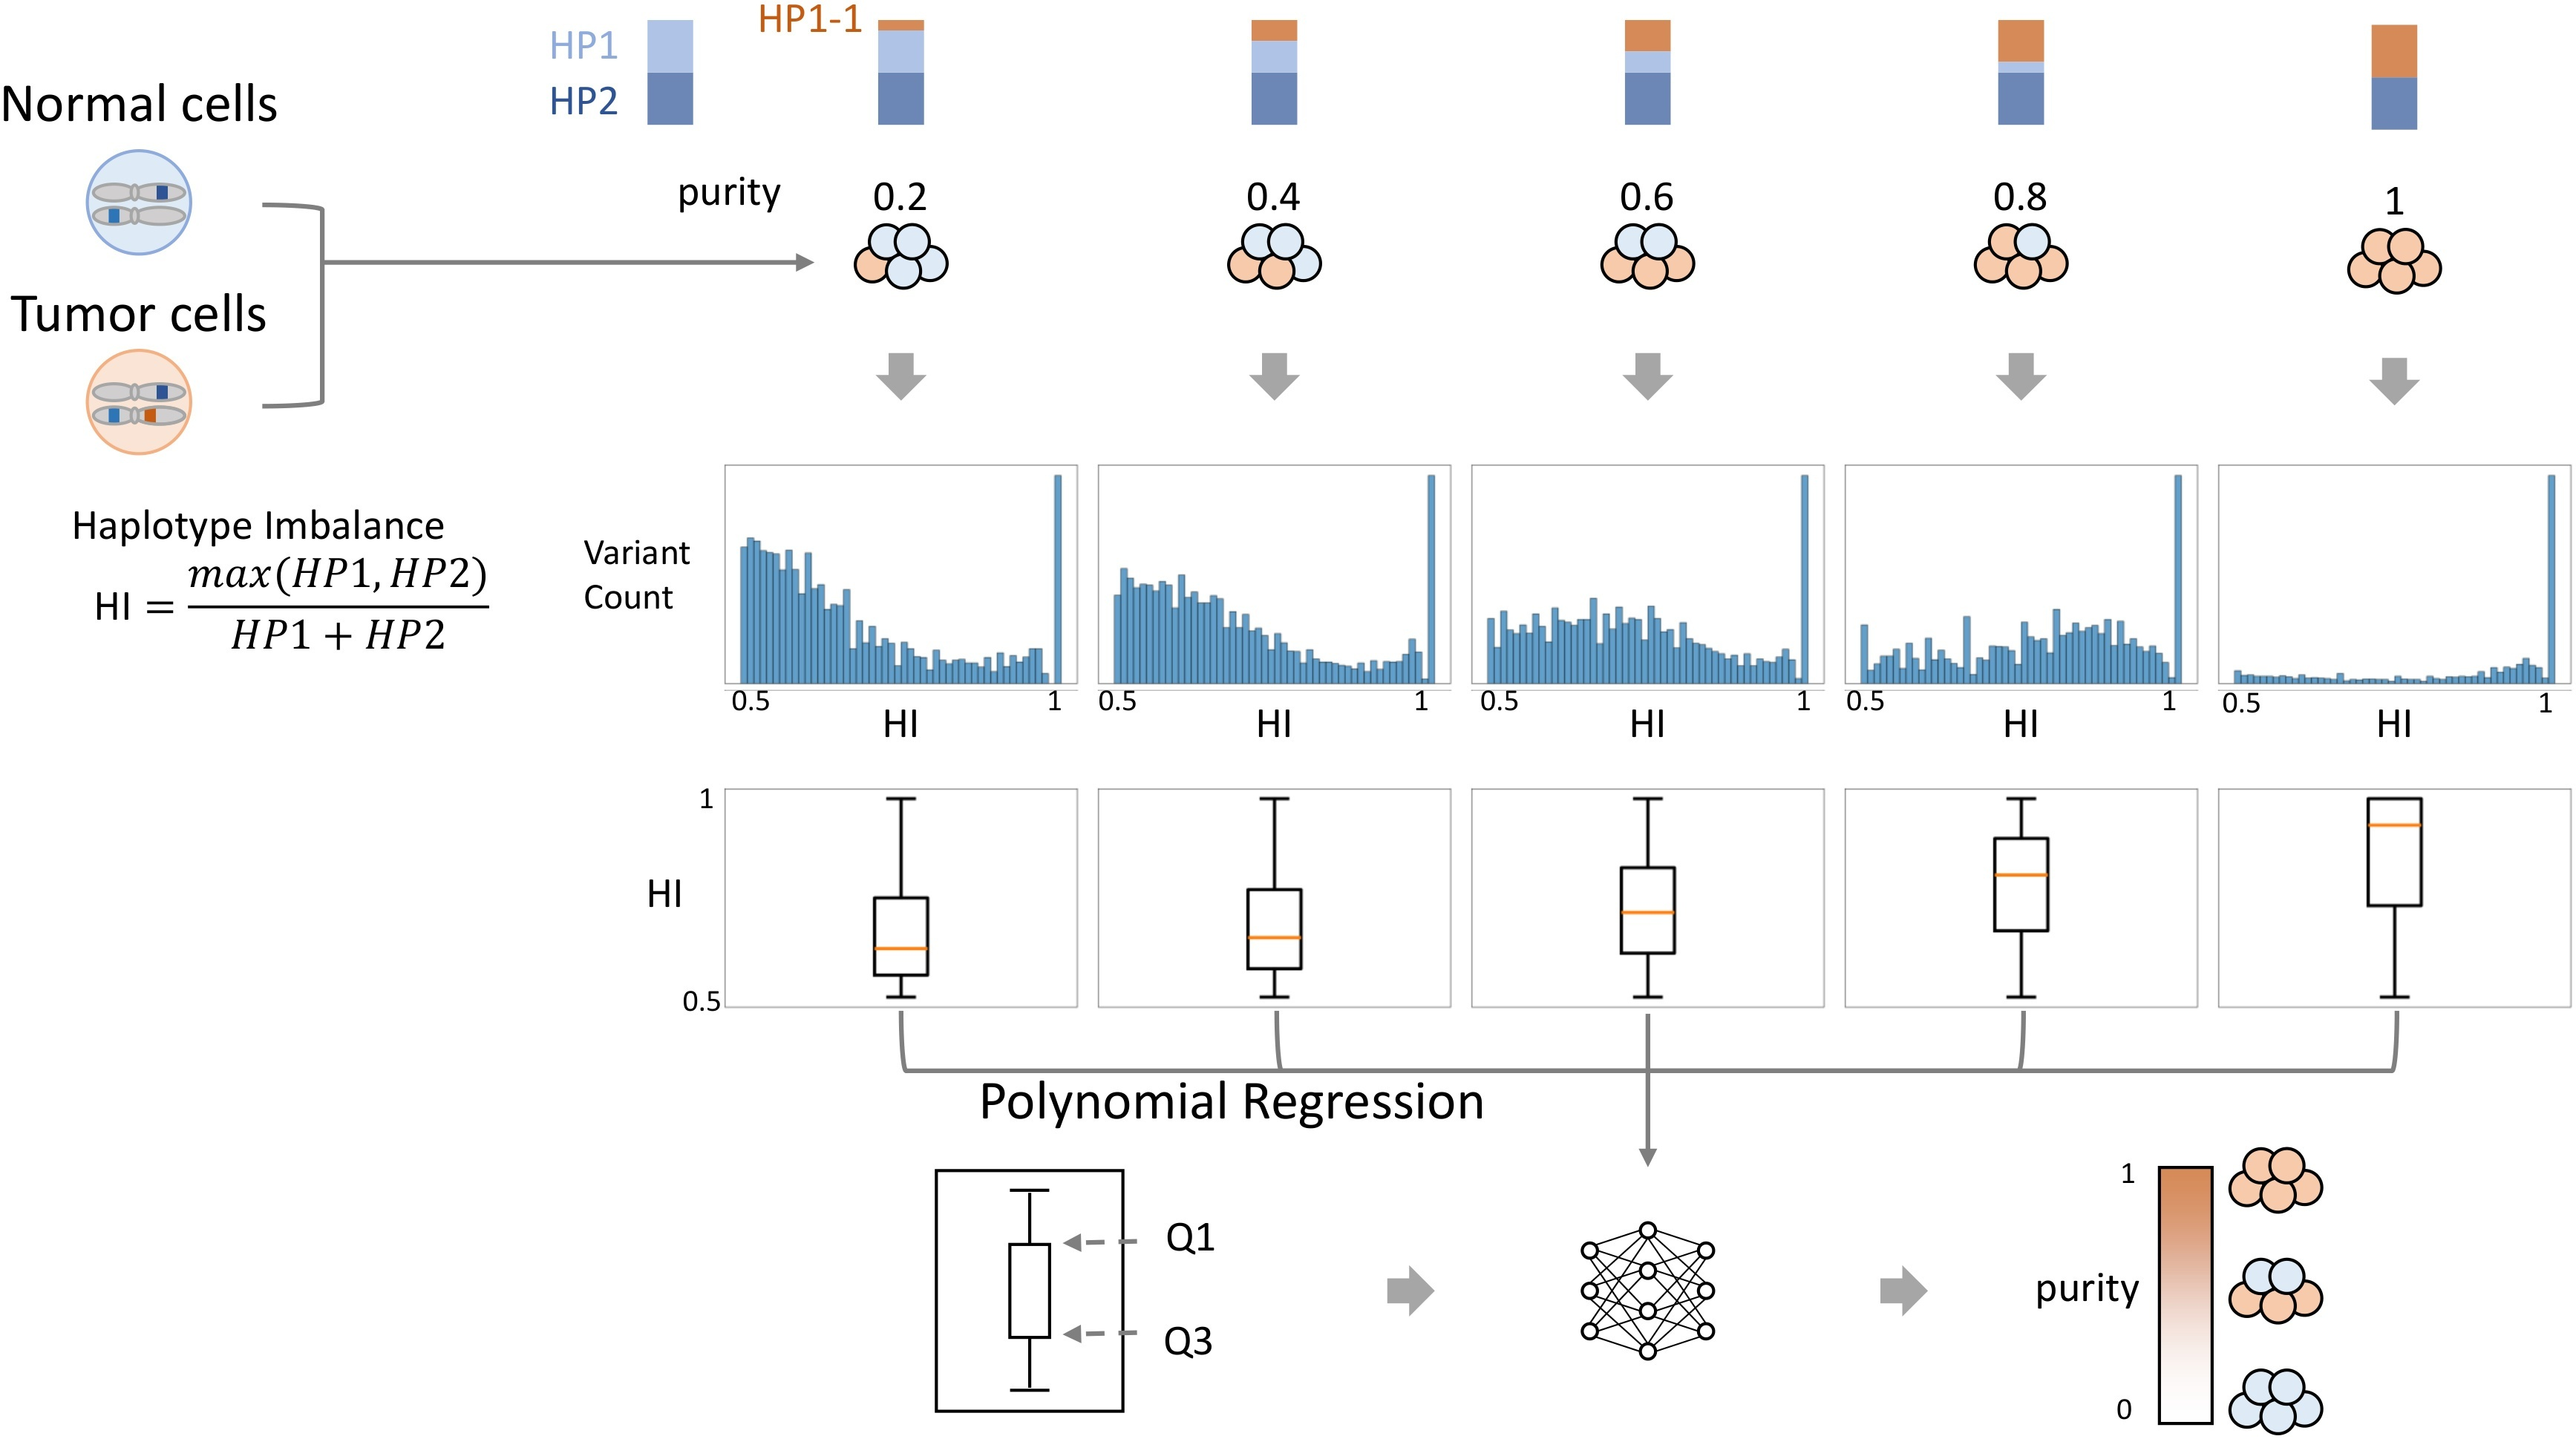
\includegraphics[keepaspectratio]{page_25_cropped.jpg}}
\caption[Haplotype Imbalance Principle]{Principle of tumor purity prediction using Haplotype Imbalance (HI). The figure shows that as tumor purity increases from 0.2 to 1.0, the proportion of somatic haplotypes increases. This causes the genome-wide distribution of HI, shown in histograms and box plots, to shift from a balanced state (centered at 0.5) to a highly imbalanced state with higher median values and a peak at 1.0.}\label{fig:met-page-25-cropped-jpg}
\end{figure}

\subsubsection{Predictive Modeling with Genomic Features}\label{predictive-modeling-with-genomic-features}

To formalize this relationship, a polynomial regression framework was applied. Two key sets of features were extracted from the genomic data. The first was the LOH Ratio, defined as the proportion of the genome affected by LOH:

$$
\text{LOH Ratio} = \frac{L_{\text{LOH}}}{L_{\text{Genome}}}
$$

where \(L_{\text{LOH}}\) denotes the total length of all detected LOH regions and \(L_{\text{Genome}}\) is the total analyzable genome length. Although the regression model primarily relied on haplotype imbalance (HI) as the main predictor, the LOH ratio provided complementary information. In particular, LOH is especially pronounced when tumor purity approaches 1, thereby improving predictive accuracy in high-purity samples.

The second feature set comprised the haplotype imbalance statistics, namely the first (Q1) and third (Q3) quartiles of the genome-wide HI distribution, which summarize the central tendency and variability of allelic imbalance. Together, these features (LOH Ratio, Q1 of HI, and Q3 of HI) were used as predictors in the polynomial regression model, which was fitted to establish the relationship between genomic features and tumor purity (Figure~\ref{fig:met-page-26-cropped-jpg}).

\begin{figure}
\centering
\pandocbounded{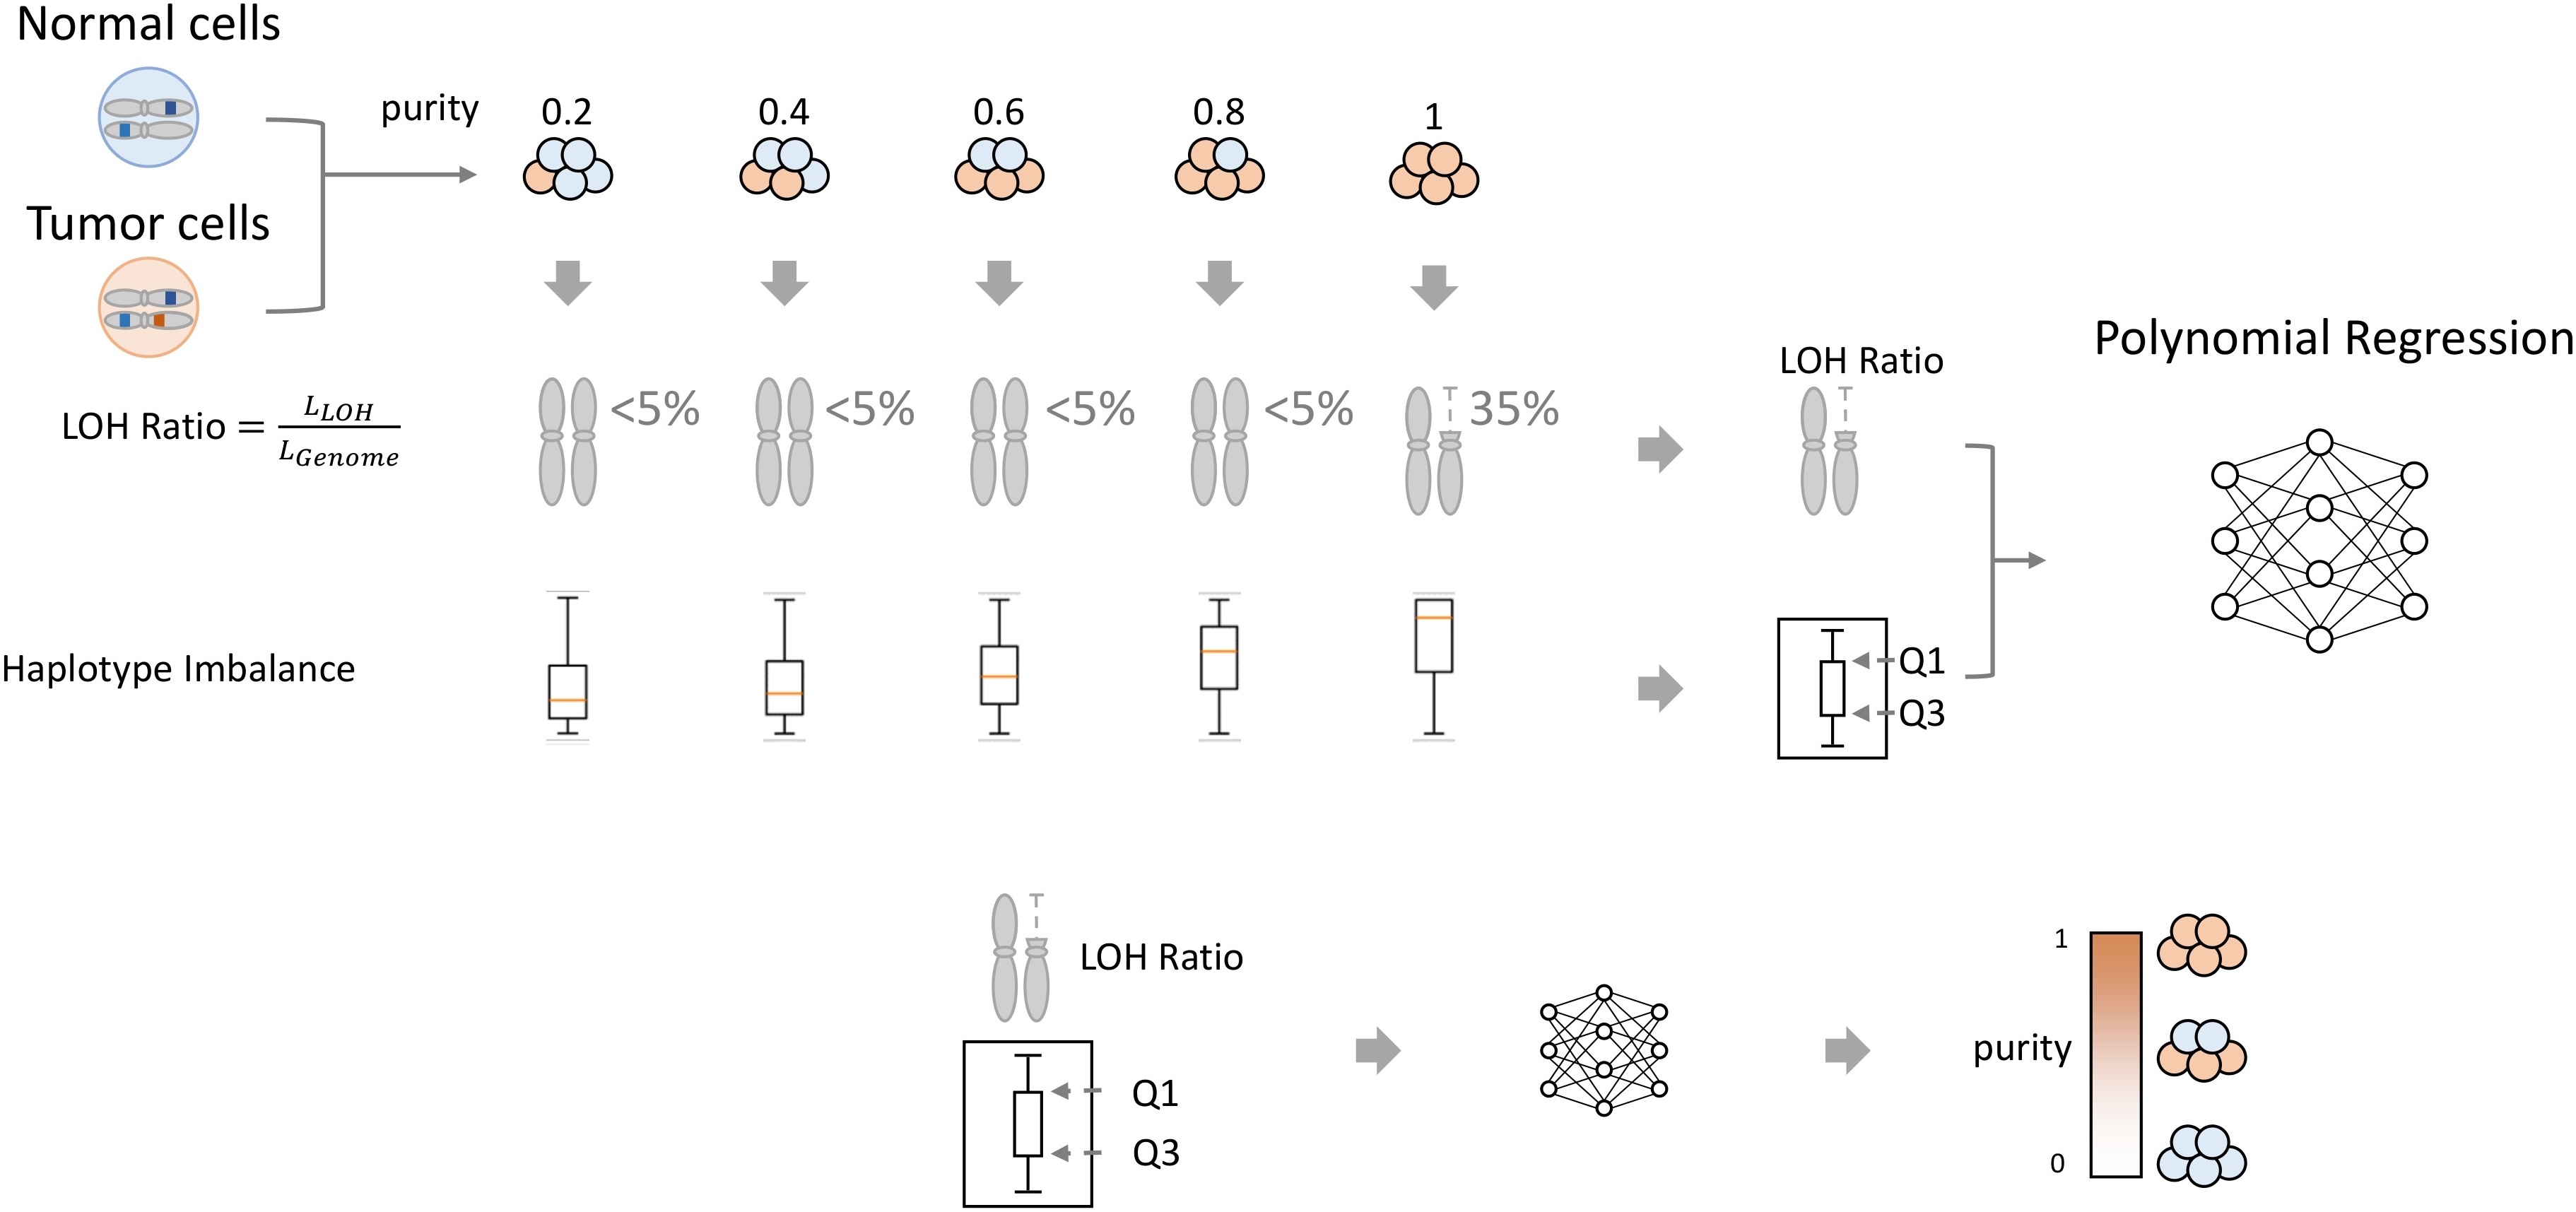
\includegraphics[keepaspectratio]{page_26_cropped.jpg}}
\caption[Tumor Purity Prediction Model]{Schematic of the tumor purity prediction model. The model takes two types of genomic features as input: the LOH Ratio (fraction of the genome with LOH) and statistics from the Haplotype Imbalance distribution (represented by the Q1 and Q3 quartiles of a box plot). These features are provided to a Polynomial Regression model, from which the estimated tumor purity is obtained.}\label{fig:met-page-26-cropped-jpg}
\end{figure}

\subsection{Data and Computational Resources}\label{data-and-computational-resources}

\subsubsection{Data Sources and Benchmark Sets}\label{data-sources-and-benchmark-sets}

This study made use of publicly available long-read sequencing data derived from a panel of well-characterized cancer cell lines. The inclusion of these standardized reference materials ensures the reproducibility of the analyses and enables rigorous benchmarking against established ground-truth call sets. The cell lines, together with their corresponding data sources and benchmark sets, are summarized in Table~\ref{tab:cell-lines}.

\begin{longtable}[]{@{}lll@{}}
\caption{Cancer cell lines used in this study, with their sequencing data sources and benchmark references.}
\label{tab:cell-lines} \\
\toprule
Cell Line & Material Source & Benchmark Source \\
\midrule
\endfirsthead
\toprule
Cell Line & Material Source & Benchmark Source \\
\midrule
\endhead
\bottomrule
\endlastfoot
COLO829 & ONT, NYGC & NYGC \\
H1437 & UCSC & Google \\
H2009 & UCSC & Google \\
HCC1395 & HKU, NYGC & SEQC2 \\
HCC1937 & UCSC & Google \\
HCC1954 & UCSC & Google \\
\end{longtable}

\subsubsection{Somatic Variant Calling Tools}\label{somatic-variant-calling-tools}

To assess the performance of the proposed pipeline, we compared it against several state-of-the-art somatic variant calling tools specifically designed for long-read sequencing and/or tumor-only analysis. The tools and their respective versions are summarized in Table~\ref{tab:callers}.

\begin{longtable}[]{@{}l@{}}
\caption{Somatic variant callers used for benchmarking.}
\label{tab:callers} \\
\toprule
Somatic Variant Callers \\
\midrule
\endfirsthead
\toprule
Somatic Variant Callers \\
\midrule
\endhead
\bottomrule
\endlastfoot
ClairS-TO v0.3.0 (ssrs) \\
ClairS-TO v0.3.0 (ss) \\
DeepSomatic v1.8.0 (tumor-only) \\
\end{longtable}

\subsubsection{Generation of In-Silico tumor–normal Mixtures}\label{generation-of-in-silico-tumor–normal-mixtures}

To test and evaluate the accuracy of variant calling under different tumor purities, and to train and validate the tumor purity prediction model, a benchmark dataset was required, with purity levels assumed to be known (assuming the pure tumor cell line has purity = 1). This dataset was generated using an in-silico titration approach. High-coverage long-read sequencing data were obtained from a pure tumor cell line and its matched normal cell line. Synthetic mixture samples were then created by downsampling the raw reads and mixing tumor and normal reads at predefined ratios under different total coverage levels (Figure~\ref{fig:met-page-27-cropped-jpg}). Specifically, five target purity levels were set: 1.0, 0.8, 0.6, 0.4, and 0.2, and corresponding mixed samples were generated at different total coverages. This procedure resulted in a benchmark dataset, where each sample was assigned a corresponding purity label, which can be used to assess the performance of variant calling and serve as a reference for training and validating tumor purity prediction models.

\begin{figure}
\centering
\pandocbounded{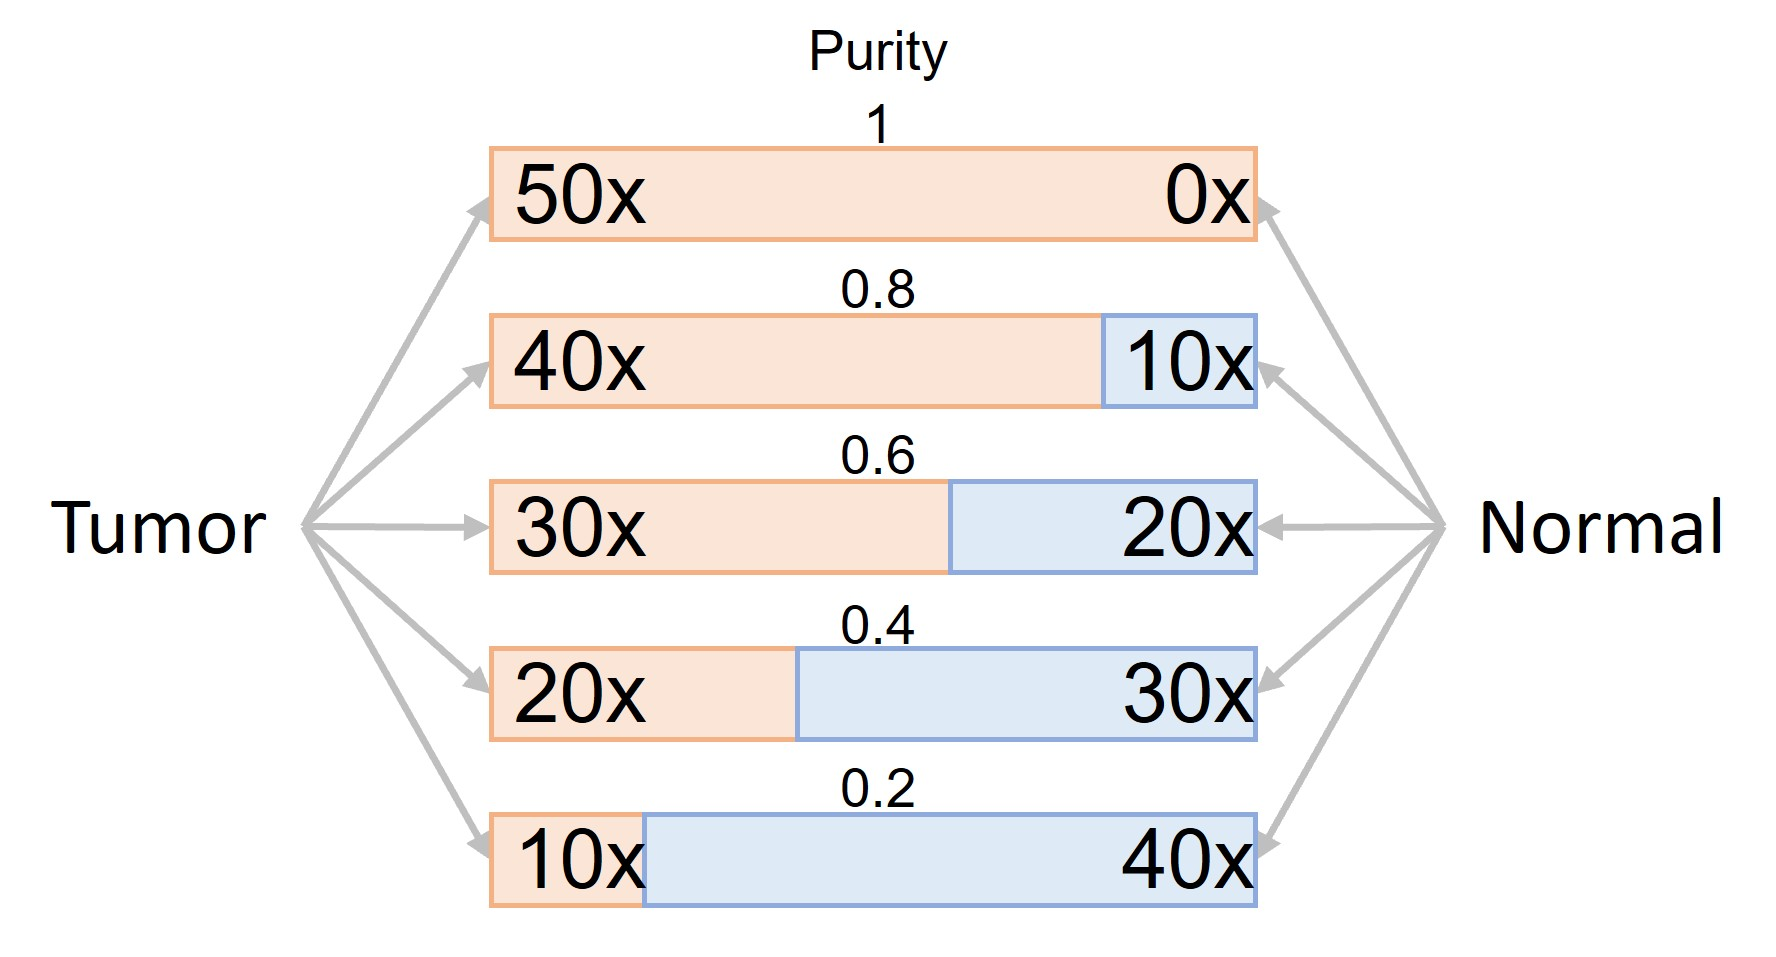
\includegraphics[width=0.6\textwidth,keepaspectratio]{page_27_cropped.jpg}}
\caption[In-Silico Mixture Generation]{Generation of in-silico tumor–normal mixtures for benchmarking. This diagram illustrates the method of creating synthetic samples with known tumor purity. Raw sequencing reads from a pure tumor sample (orange) and a pure normal sample (blue) are mixed in specific proportions to create samples with precise purity levels (e.g., 0.8 purity from 40x tumor and 10x normal reads), providing a ground-truth dataset for model training and validation.}\label{fig:met-page-27-cropped-jpg}
\end{figure}

\section{Appendix}\label{appendix}

\subsection{Supplementary Methods for Somatic Variant Analysis}\label{supplementary-methods-for-somatic-variant-analysis}

This appendix provides supplementary details on the computational methodologies developed and employed for the detection of somatic variants and structural alterations from long-read sequencing data. The sections below describe the algorithms for Loss of Heterozygosity (LOH) detection, the rationale and implementation of pattern-based filtering for somatic variant calls, the integrated workflow for variant analysis, and a case study demonstrating the application of these methods.

\subsubsection{Methodology for Loss of Heterozygosity (LOH) Detection}\label{methodology-for-loss-of-heterozygosity-loh-detection}

Loss of Heterozygosity (LOH) is a common genomic event in cancer wherein one parental allele of a chromosome segment is lost. To detect LOH regions, we developed a two-step classification method based on the local density of heterozygous variants. The approach first assigns a genotype to each variant based on its allele frequency and then calculates a Heterozygosity Ratio \(H_r\) for genomic windows to classify them as LOH or Non-LOH (Figure~\ref{fig:app-page-37-cropped-jpg}).

The determination of classification thresholds was guided by empirical distributions of the data. As shown in Figure~\ref{fig:app-page-37-cropped-jpg}a, the violin plot illustrates the distribution of Variant Allele Frequencies (VAF) for variants located within predefined LOH (green) and Non-LOH (blue) regions. In Non-LOH regions, the VAF distribution is bimodal, with a prominent peak at 0.5 representing heterozygous variants and a smaller peak near 1.0 corresponding to homozygous variants. By contrast, LOH regions exhibit a unimodal distribution strongly skewed towards 1.0, consistent with the loss of one allele and the concomitant depletion of heterozygous variants. Based on these empirical patterns, a threshold of VAF ≥ 0.8 was selected to classify variants as homozygous in subsequent analyses.

Similarly, Figure~\ref{fig:app-page-37-cropped-jpg}b presents a box plot of the Heterozygosity Ratio for regions classified as LOH and Non-LOH. The ratio, defined as the proportion of heterozygous variants within a genomic window, shows a clear separation between the two groups. Non-LOH regions consistently display higher values with a median around 0.55, whereas LOH regions approach zero. On the basis of this distribution, a threshold of $H_r = 0.09$ was established to distinguish LOH from Non-LOH regions.

This quantitative framework, supported by empirical observations of allele frequency and heterozygosity ratio distributions, provides a robust and automated method for identifying LOH events across the genome by leveraging the statistical signature of heterozygote depletion.

\begin{figure}
\centering
\pandocbounded{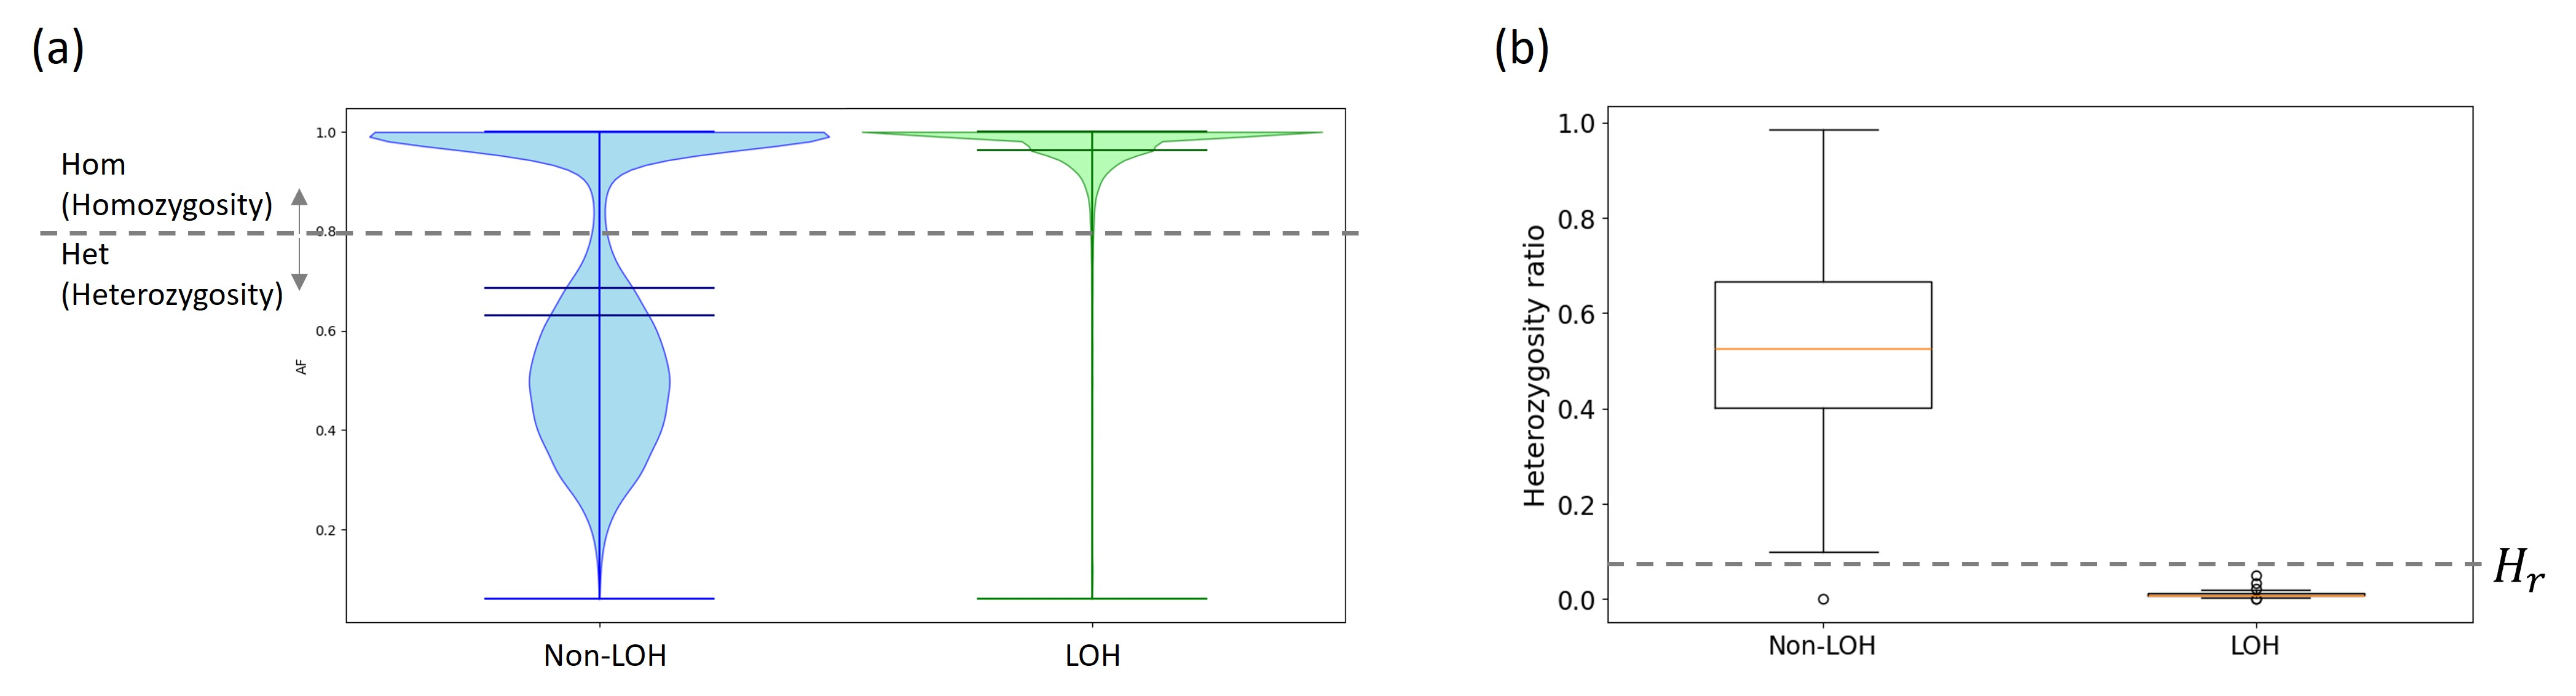
\includegraphics[keepaspectratio]{page_37_cropped.jpg}}
\caption[LOH Detection Methodology]{A two-panel plot illustrating the methodology for Loss of Heterozygosity (LOH) detection. (a) The violin plot shows the distribution of Variant Allele Frequencies (VAF) in Non-LOH (blue) and LOH (green) regions, demonstrating that LOH regions lack the characteristic heterozygous peak at VAF=0.5. (b) The box plot shows the distribution of the calculated Heterozygosity Ratio for the two region types, revealing a clear separation that allows for robust classification using a threshold (Hr = 0.09).}\label{fig:app-page-37-cropped-jpg}
\end{figure}

\subsubsection{Pattern-Based Filtering for Somatic Variant Calling}\label{pattern-based-filtering-for-somatic-variant-calling}

Alongside the detection of large-scale genomic events, the accurate identification of individual somatic variants is a critical objective that is frequently challenged by sequencing artifacts and other sources of noise. To address this challenge, we developed a filtering strategy that evaluates the specific patterns of evidence supporting each candidate variant. This approach is based on the rationale that true somatic mutations exhibit characteristic, high-confidence evidence patterns that differ from those of artifacts.

\paragraph{Rationale for Pattern-Based Evidence Selection}\label{rationale-for-pattern-based-evidence-selection}

The rationale for selecting specific evidence patterns is grounded in their empirical association with variant call accuracy rather than arbitrary design. As shown in Figure~\ref{fig:app-page-38-cropped-jpg}, predefined patterns were evaluated by comparing their relative abundance across validated true positive (TP) and false positive (FP) variant sets. The analysis revealed that \(V_H\) (high-confidence) patterns are strongly enriched for TPs with minimal FP contribution, while \(V_L\) (low-confidence) patterns, although less frequent, remain reliable indicators of true variants. In contrast, \(V_N\) (non-somatic) patterns, dominated by the `DISAGREE' category, contribute substantially to both TPs and FPs, rendering them unreliable. These findings demonstrate that the prioritization of \(V_H\) and \(V_L\) patterns is empirically justified and provides a principled basis for the filtering strategy.

\begin{figure}
\centering
\pandocbounded{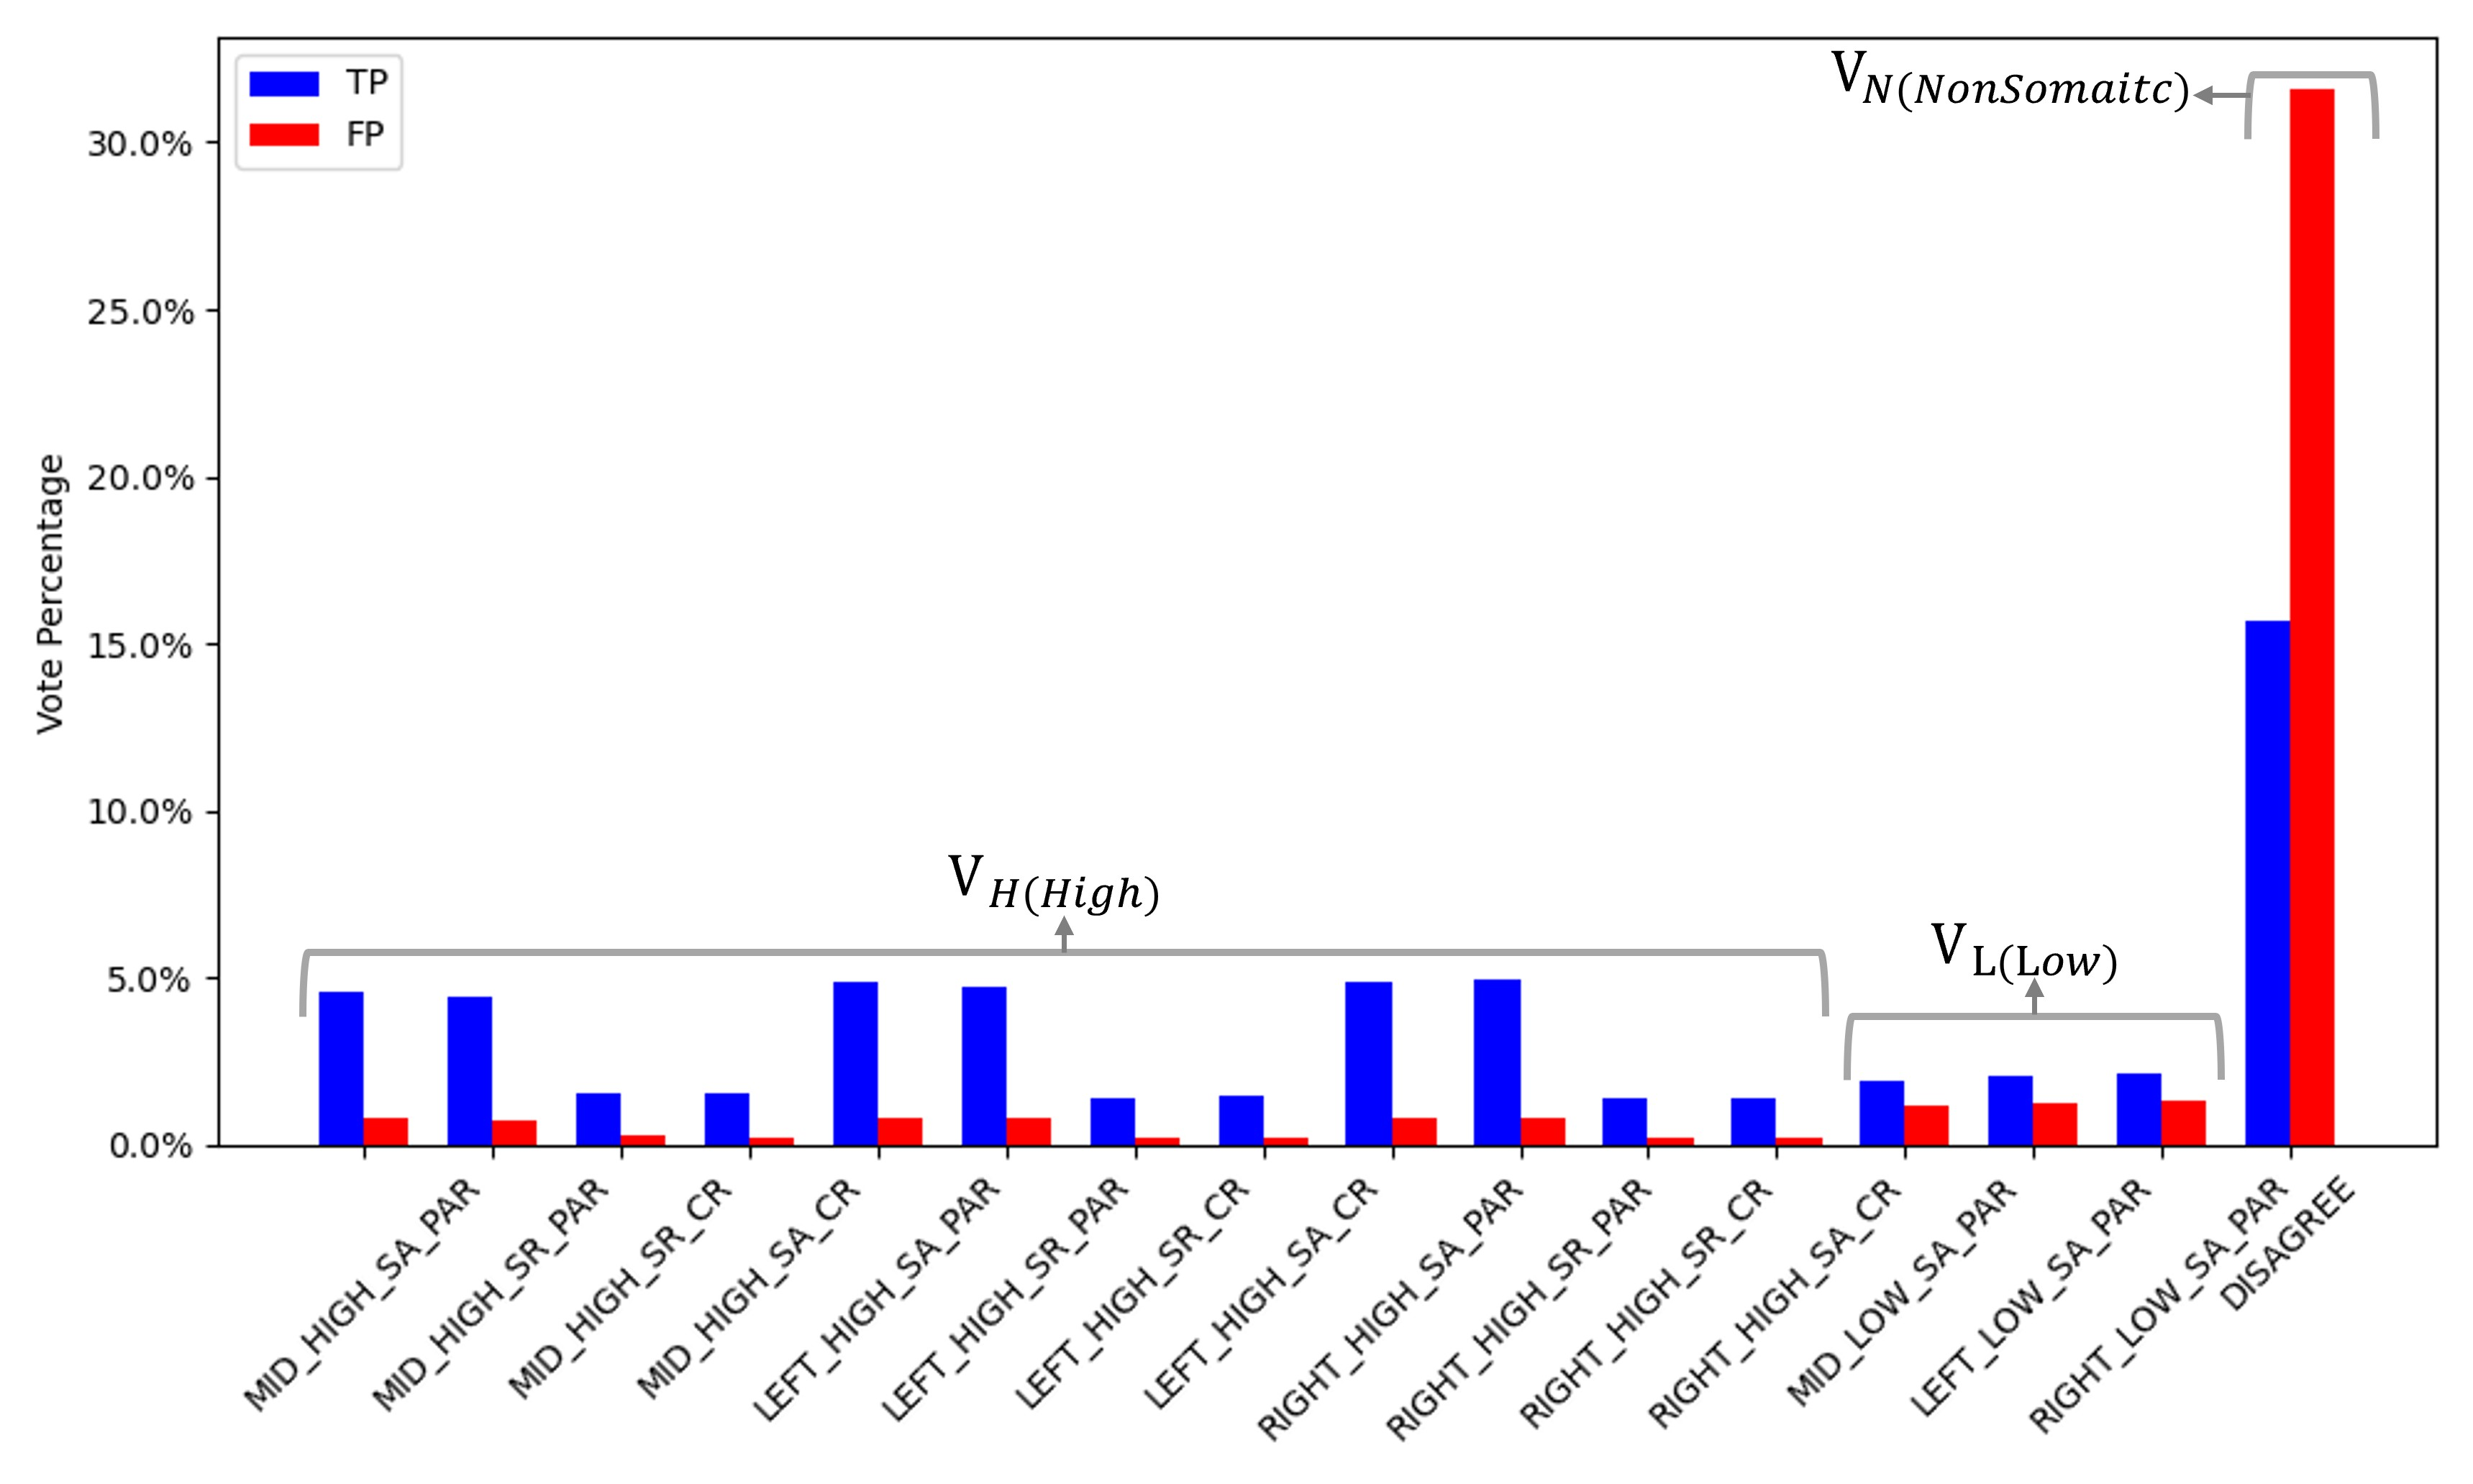
\includegraphics[keepaspectratio]{page_38_cropped.jpg}}
\caption[Evidence Pattern Comparison]{Comparison of True Positive (TP, blue) and False Positive (FP, red) variant calls across predefined evidence patterns. The patterns are grouped into three categories: high-confidence (\(V_H\)), low-confidence (\(V_L\)), and non-somatic (\(V_N\)). \(V_H\) patterns are strongly enriched for TPs with minimal FP contribution, \(V_L\) patterns occur less frequently but remain reliable indicators of true variants, and \(V_N\) patterns are dominated by the DISAGREE' category, which contributes substantially to both TPs and FPs and is therefore ambiguous and unreliable. These distributions provide the rationale for adopting a filtering strategy that prioritizes variants supported by \(V_H\) and \(V_L\) patterns.}\label{fig:app-page-38-cropped-jpg}
\end{figure}

\paragraph{Pattern Artifact Filtering using a Somatic Path Ratio}\label{pattern-artifact-filtering-using-a-somatic-path-ratio}

To evaluate the robustness of the Somatic Path Ratio as a filtering criterion, we systematically compared its distribution across validated true positive (TP) and false positive (FP) variant calls (Figure~\ref{fig:app-page-39-cropped-jpg}). As illustrated, TP variants are strongly enriched near a ratio of 1.0, whereas FP variants exhibit a broader and lower distribution. This clear separation indicates that the Somatic Path Ratio provides a reliable metric for discriminating true somatic mutations from sequencing artifacts.

The choice of the threshold \(\tau\) was guided by empirical data. By analyzing the overlap of TP and FP distributions, a cutoff of approximately \(\tau = 0.8\) was identified as an optimal balance. At this threshold, a portion of FP calls can be effectively excluded while preserving high sensitivity for TP variants. Importantly, this cutoff minimizes the trade-off between precision and recall, ensuring that filtering improves accuracy without substantial loss of sensitivity.

Overall, these analyses support the use of \(\tau = 0.8\) as a data-driven threshold derived from the empirical distributions of TP and FP calls. The application of this threshold enhances the reliability of variant filtering while maintaining broad sensitivity in detection.

\begin{figure}
\centering
\pandocbounded{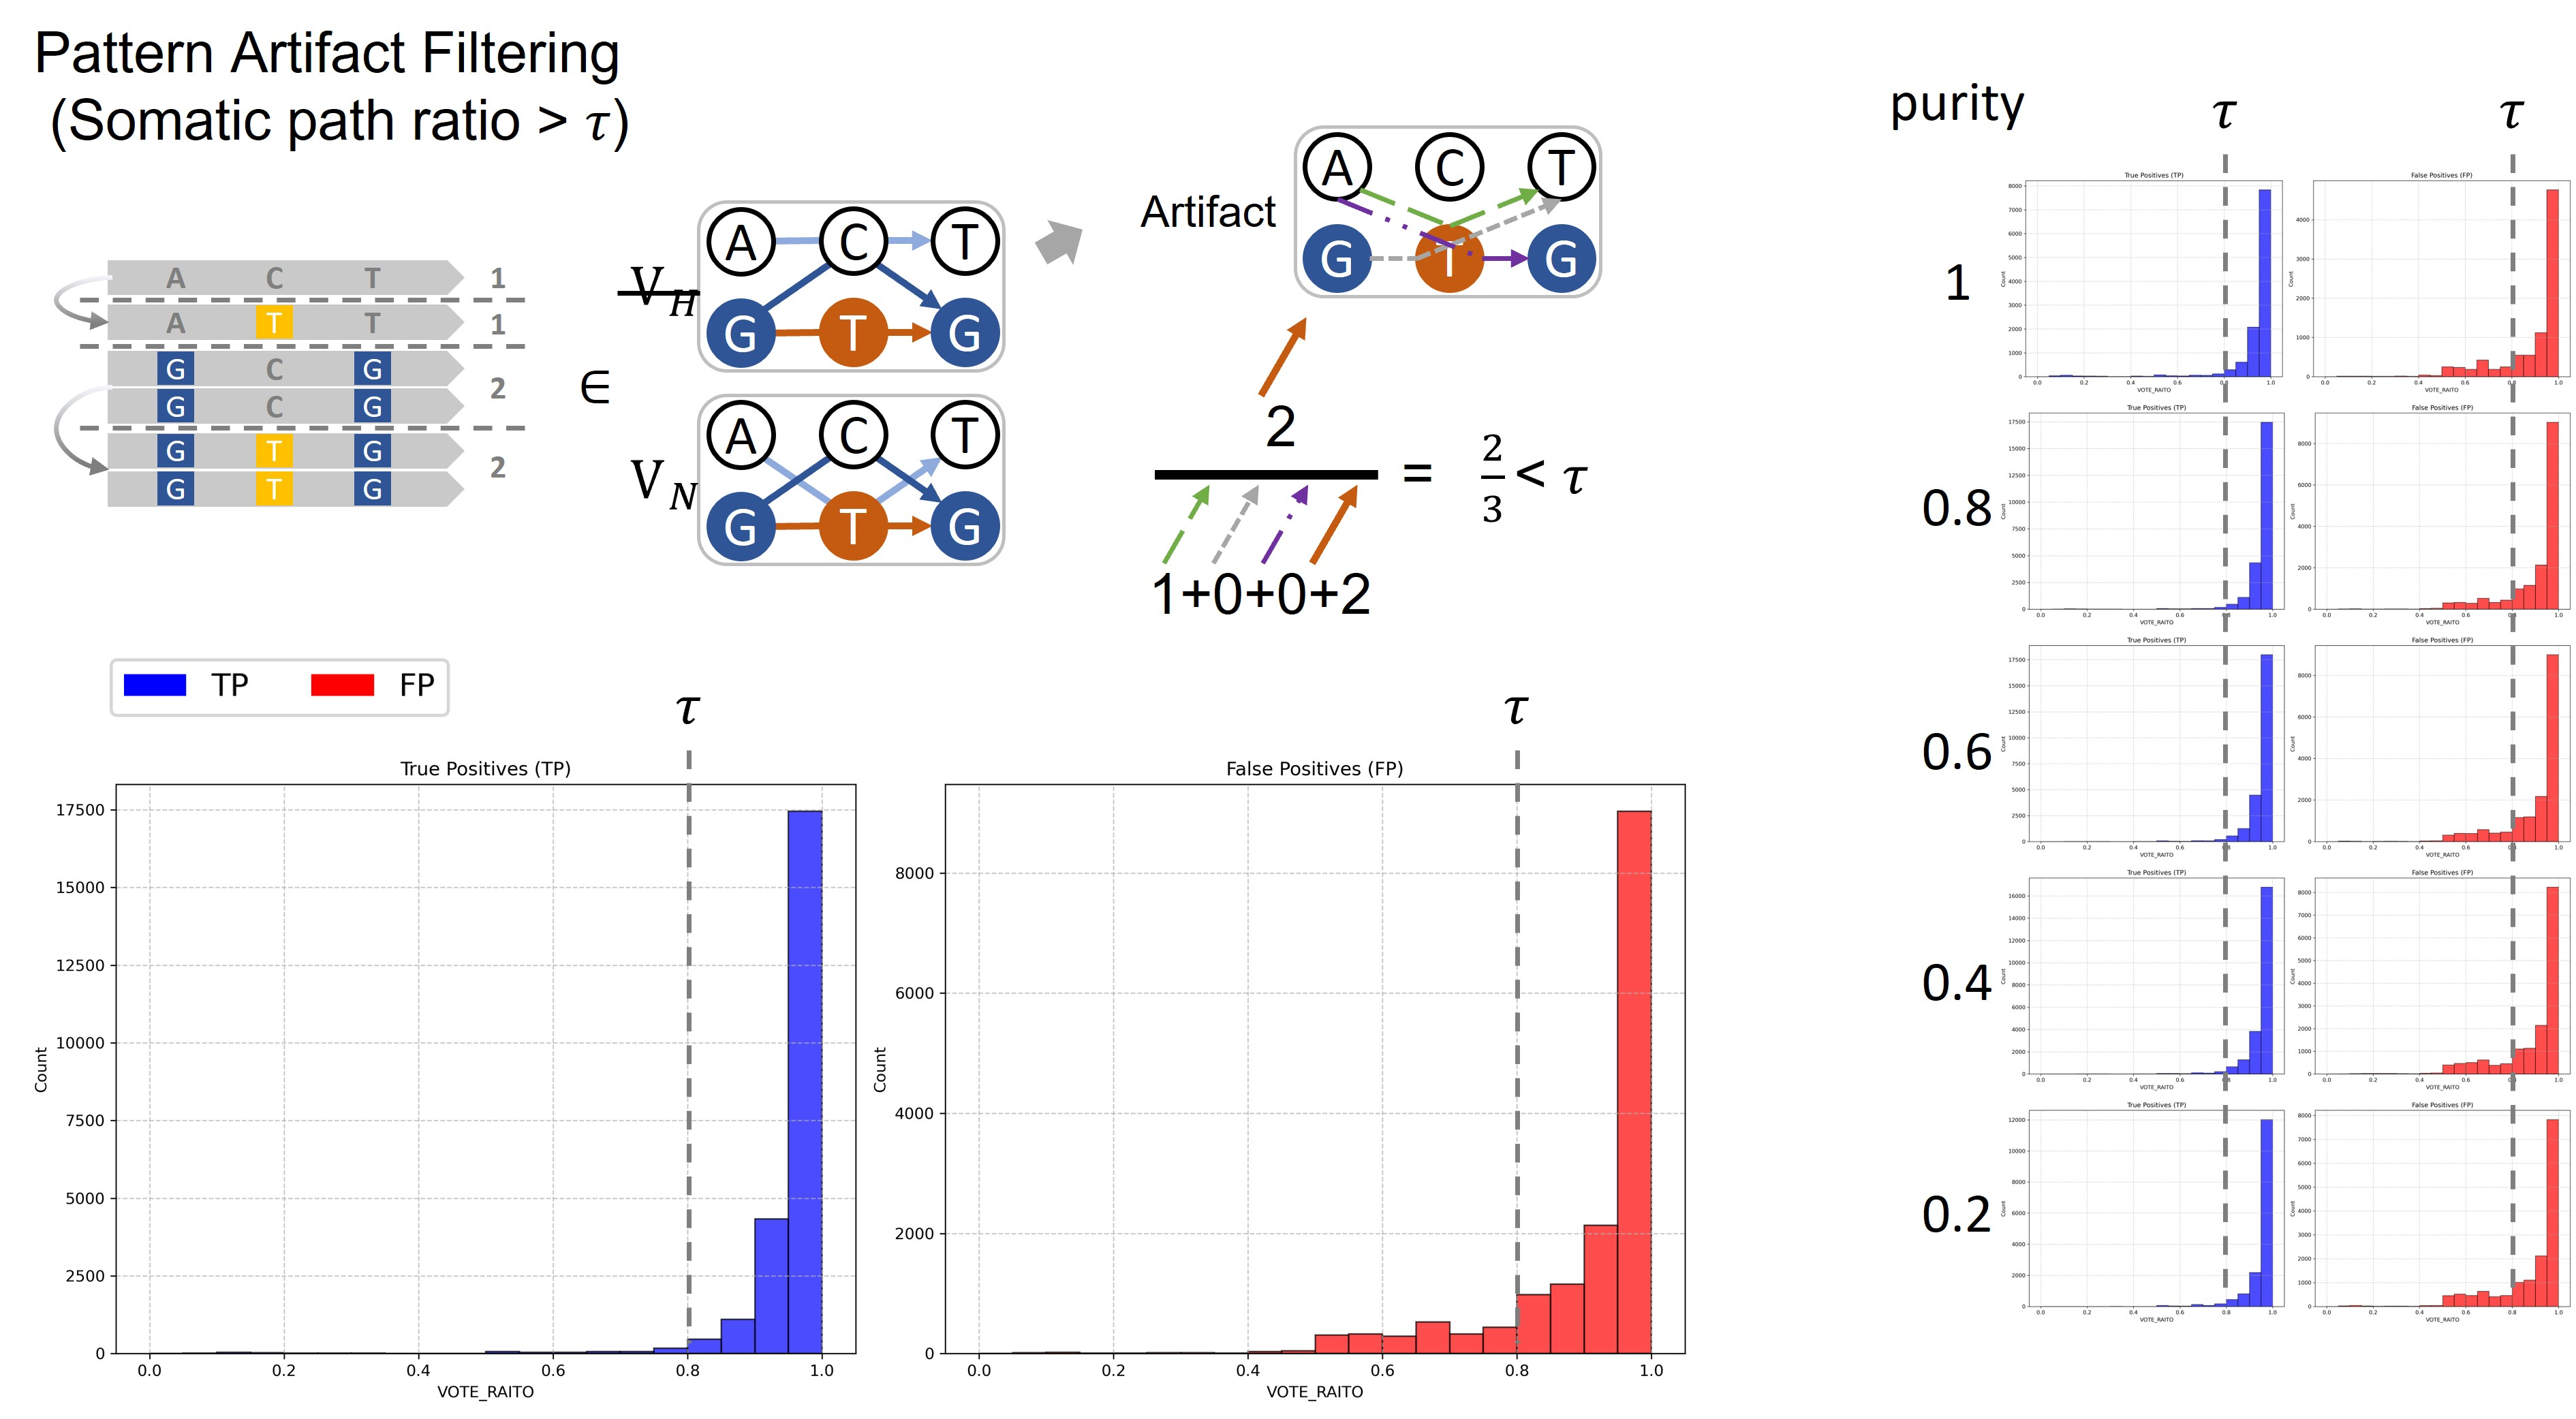
\includegraphics[keepaspectratio]{page_39_cropped.jpg}}
\caption[Somatic Path Ratio Distribution]{Distribution and robustness of the Somatic Path Ratio for artifact filtering. The histograms show that true positives (TP, blue) consistently have a high ratio near 1.0, whereas false positives (FP, red) have a lower, more dispersed distribution, enabling effective filtering with a threshold \(\tau \approx 0.8\). Additional plots demonstrate this separation is maintained across a wide range of tumor purities (1.0 to 0.2).}\label{fig:app-page-39-cropped-jpg}
\end{figure}

\paragraph{Low-Confidence Variant Detection using Vlow Ratio}\label{low-confidence-variant-detection-using-vlow-ratio}

For variants supported by less definitive evidence patterns (\(V_L\)), an auxiliary filtering criterion was introduced. This measure is defined as the proportion of supporting evidence for the low-confidence variant path (\(V_L\)) relative to the total evidence from both the variant (\(V_L\)) and non-variant (\(V_N\)) paths:

$$
\frac{V_L}{V_L + V_N} \geq \theta
$$

To establish an appropriate threshold, the distribution of this measure was compared across validated true positive (TP) and false positive (FP) calls (Figure~\ref{fig:app-page-40-cropped-jpg}). FP variants are predominantly concentrated near zero, whereas TP variants display a broader distribution extending toward higher values. This separation enables the application of a threshold to reduce FP calls while retaining the majority of TP calls.

Empirical analysis indicated that a cutoff of approximately \(\theta = 0.2\) provides a suitable balance: it effectively removes a considerable fraction of FP calls while largely preserving TP sensitivity. Furthermore, the FP distribution remains narrowly centered at zero across different tumor purity levels, whereas the TP distribution shifts moderately toward lower values. These findings support the adoption of \(\theta \approx 0.2\) as a robust filtering criterion across heterogeneous sample contexts.

\begin{figure}
\centering
\pandocbounded{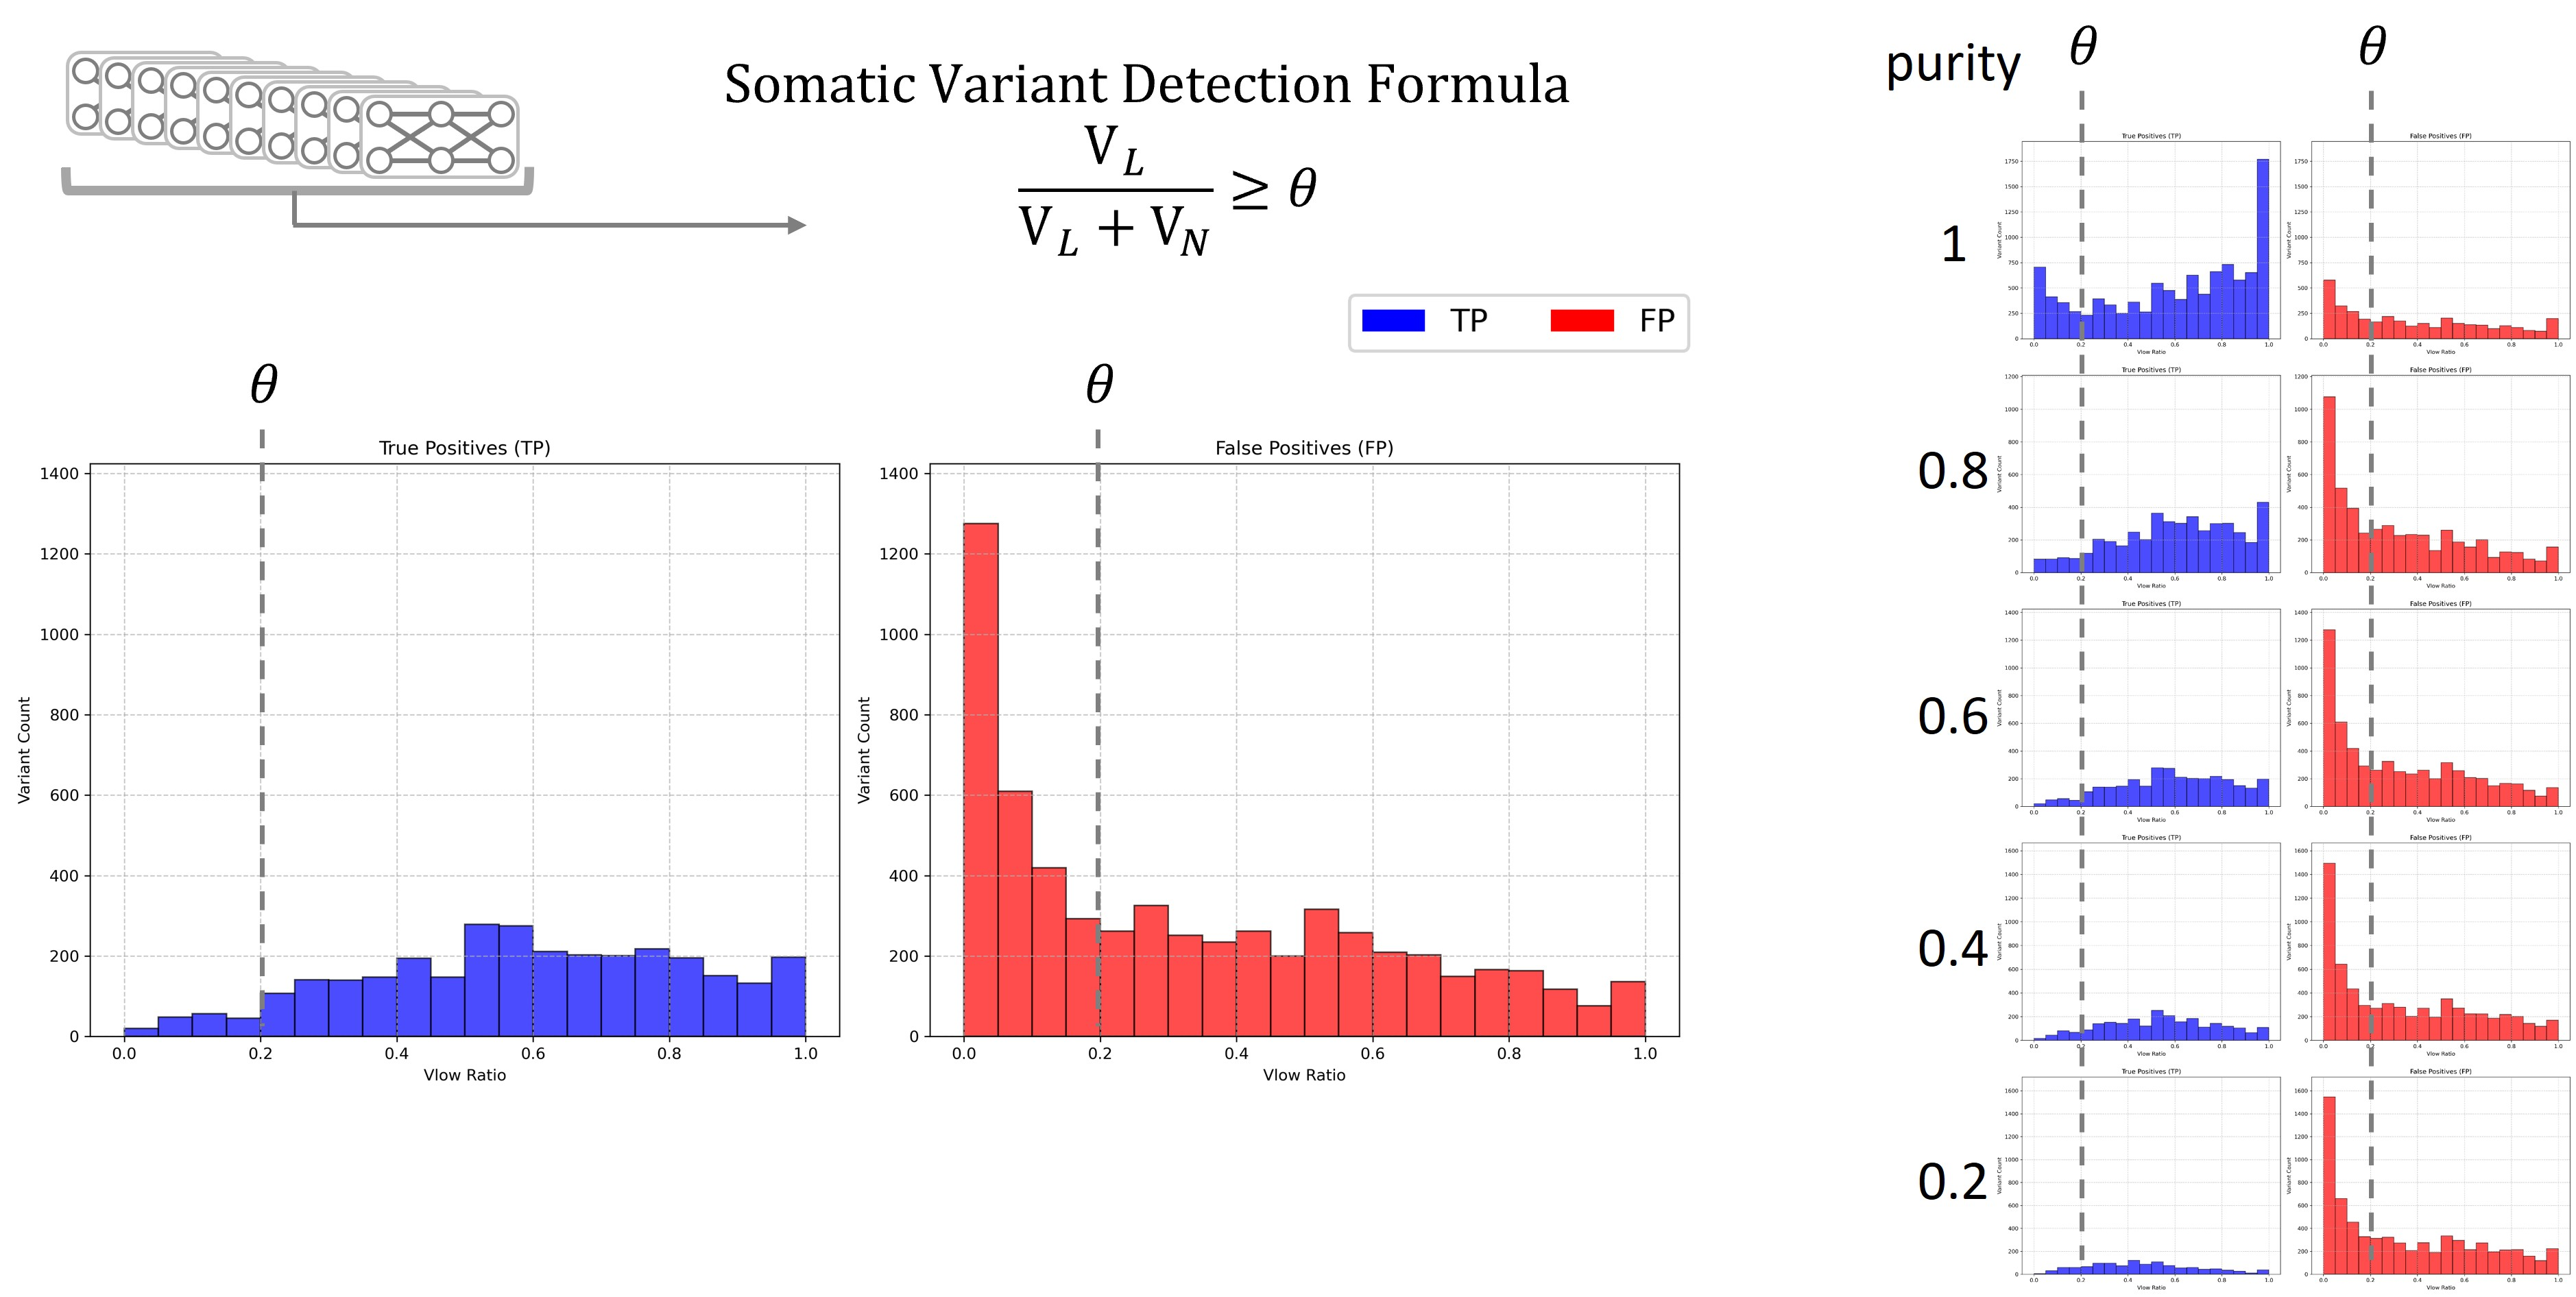
\includegraphics[keepaspectratio]{page_40_cropped.jpg}}
\caption[Low-confidence variant filtering using $V_{low}$ ratio.]{Distribution of the $V_{low}$ ratio for validated true positives (TP, blue) and false positives (FP, red). A threshold \(\theta \approx 0.2\) (dashed line) separates FP calls, which are predominantly concentrated near zero, from TP calls, which extend toward higher values. The left panels show TP distributions, and the right panels show FP distributions, across varying tumor purity levels (1.0 to 0.2). This analysis indicates that \(\theta \approx 0.2\) provides a robust filtering criterion, effectively reducing FP calls while preserving TP sensitivity across heterogeneous purity contexts.}\label{fig:app-page-40-cropped-jpg}
\end{figure}

\subsection{Purity-Aware Workflow Considerations}
\label{app:purity-aware-workflow}

The core principle underlying our method lies in the distinct behavior of germline and somatic variant allele frequencies (VAFs) in tumor--normal mixed samples. Specifically, the VAF of a heterozygous somatic variant is directly proportional to tumor purity, whereas the VAF of a heterozygous germline variant remains approximately 0.5 and is comparatively insensitive to purity (Figure~\ref{fig:app-page-41-cropped-jpg}). This statistical contrast forms the basis for separating somatic from germline signals.

At high purity, however, the VAF distributions of somatic and germline variants substantially overlap, rendering their separation statistically challenging. To address this, the workflow in (Figure~\ref{fig:app-page-42-cropped-jpg}) adopts a conditional strategy. For samples not classified as high purity, somatic variant calling proceeds after candidate selection and phasing, and the pipeline terminates accordingly. For high-purity samples, the conventional somatic variant calling step is bypassed to prevent loss of recall; instead, evidence from loss-of-heterozygosity (LOH) detection is iteratively incorporated to refine haplotype phasing and maintain analytical robustness.

\begin{figure}
\centering
\pandocbounded{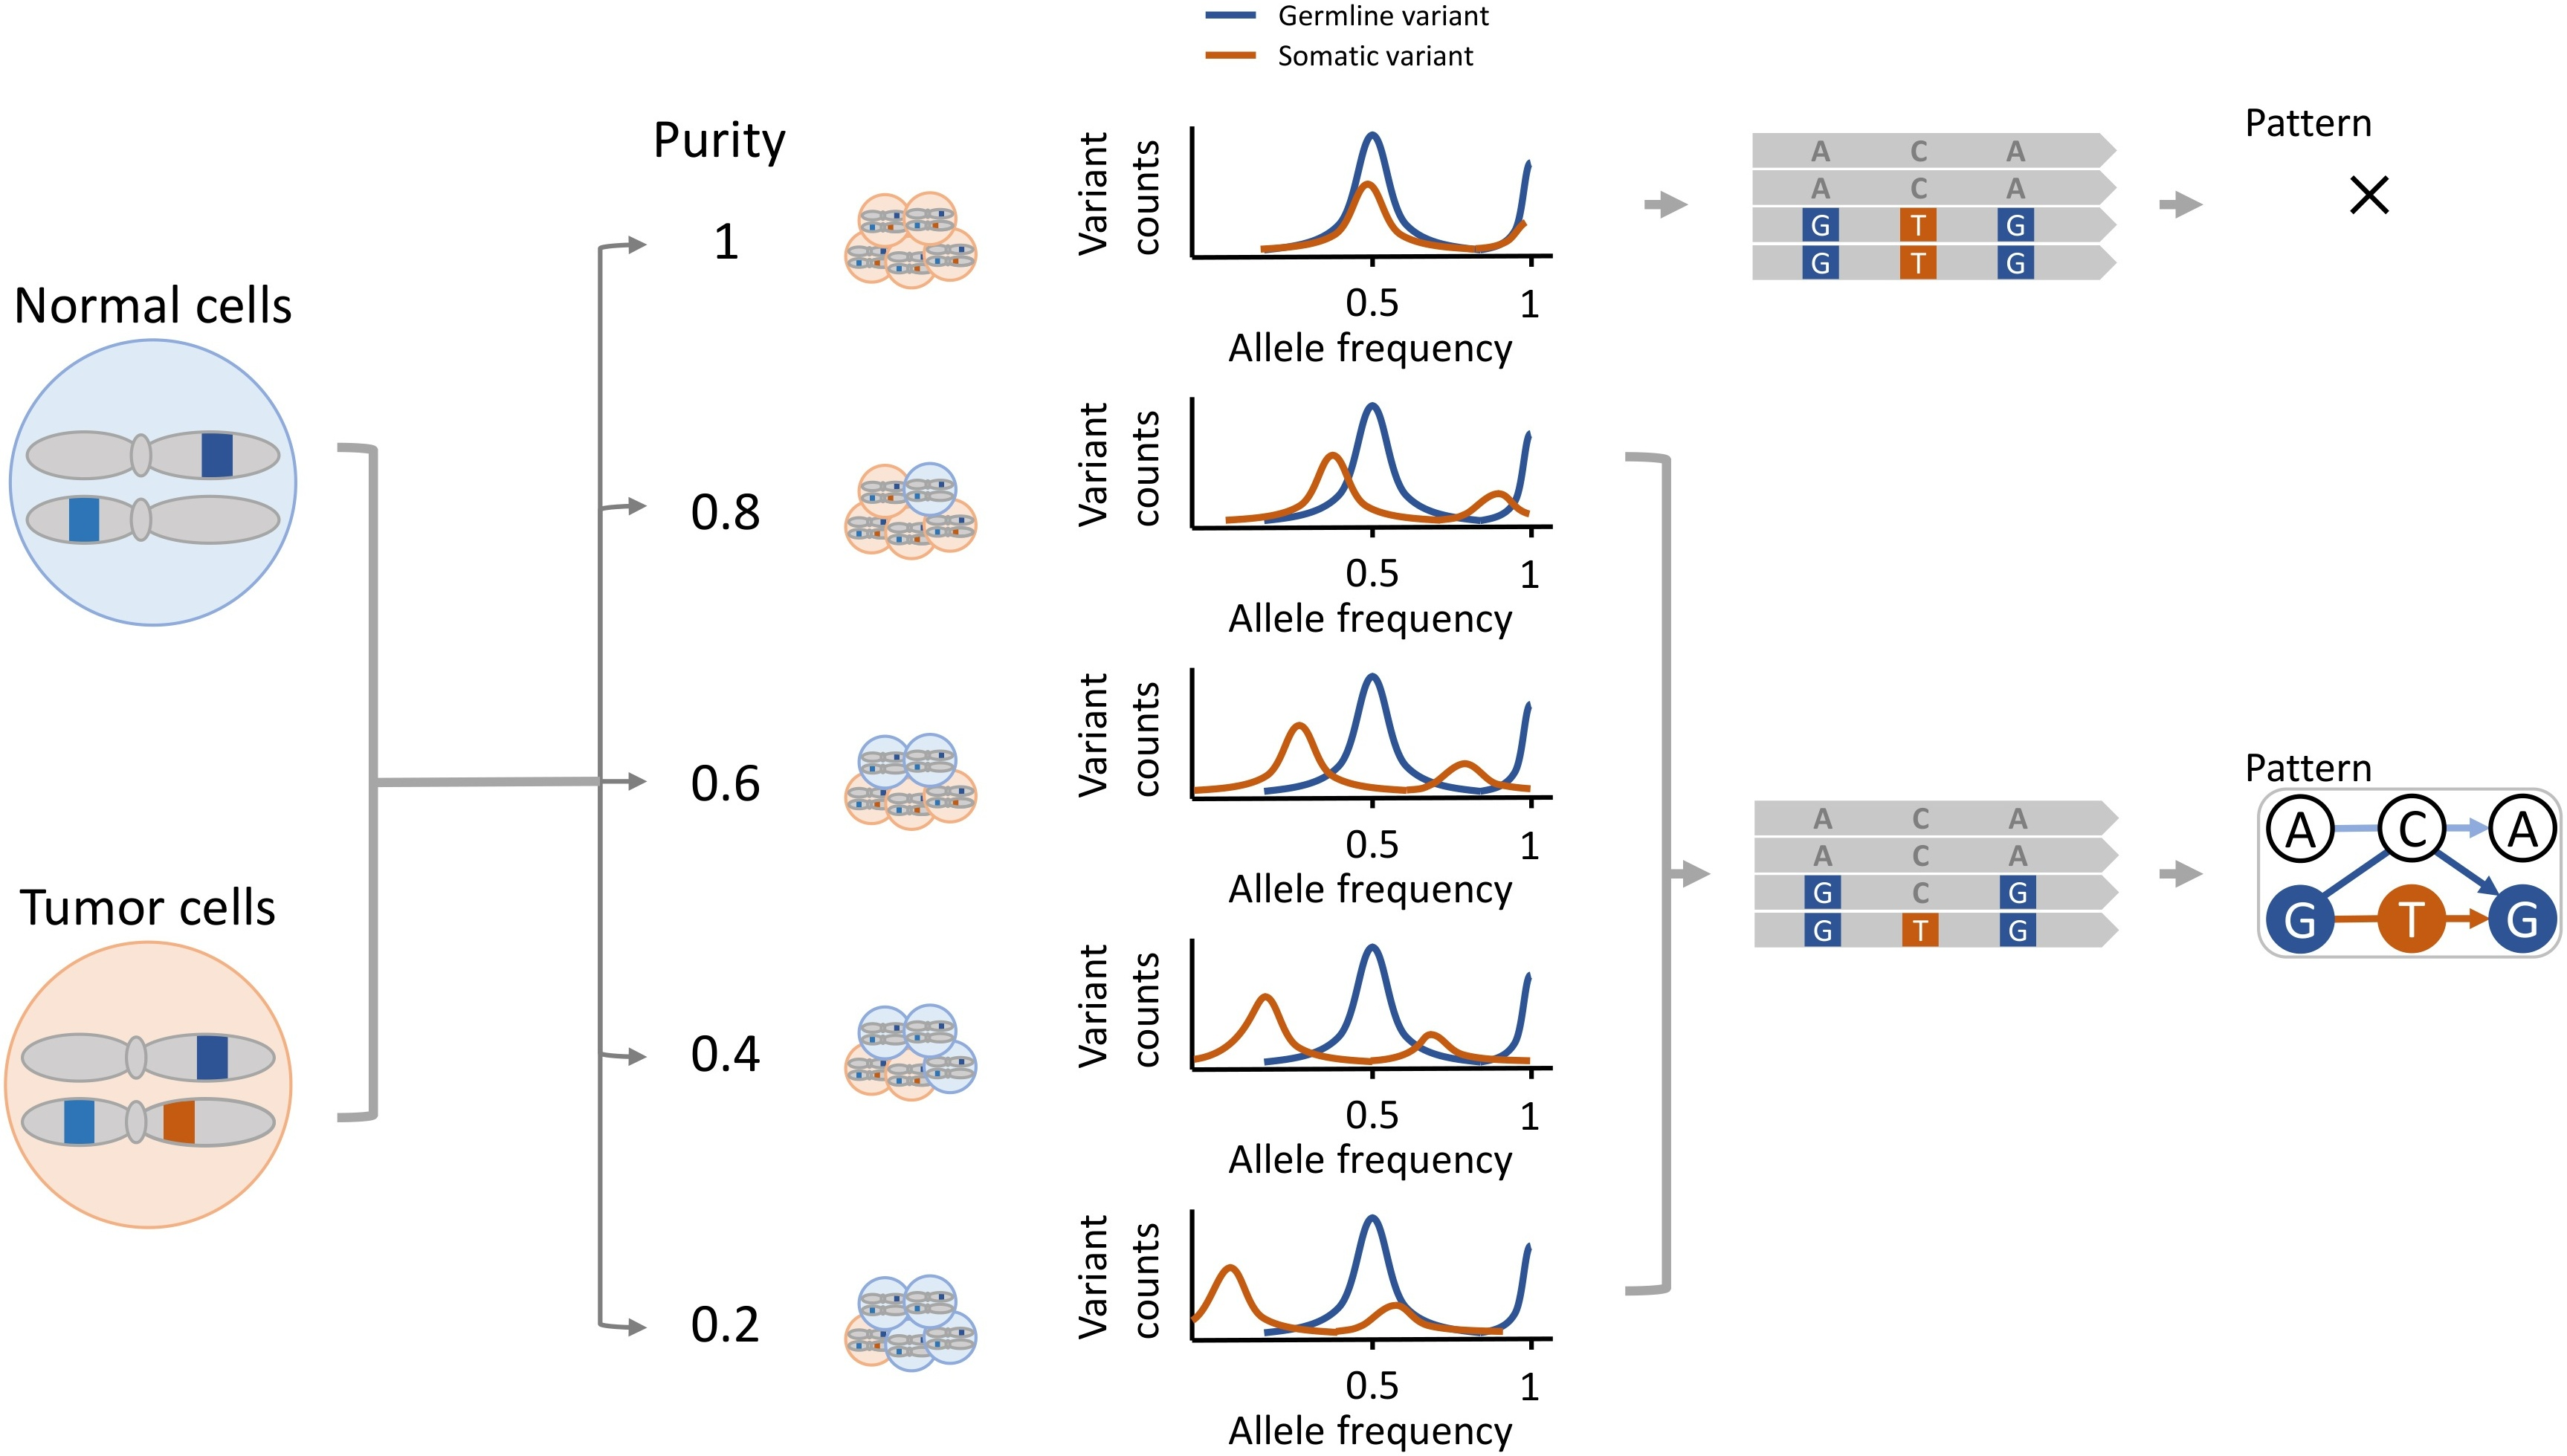
\includegraphics[keepaspectratio]{page_41_cropped.jpg}}
\caption[Tumor Purity Effect on Allele Frequencies]{Effect of tumor purity on variant allele frequencies (VAFs). The VAF of a heterozygous germline variant remains stable at approximately 0.5 across purity levels, whereas the VAF of a heterozygous somatic variant decreases proportionally with decreasing purity. At high purity, the distributions of somatic and germline variants overlap, complicating statistical separation.}\label{fig:app-page-41-cropped-jpg}
\end{figure}

\begin{figure}
\centering
\pandocbounded{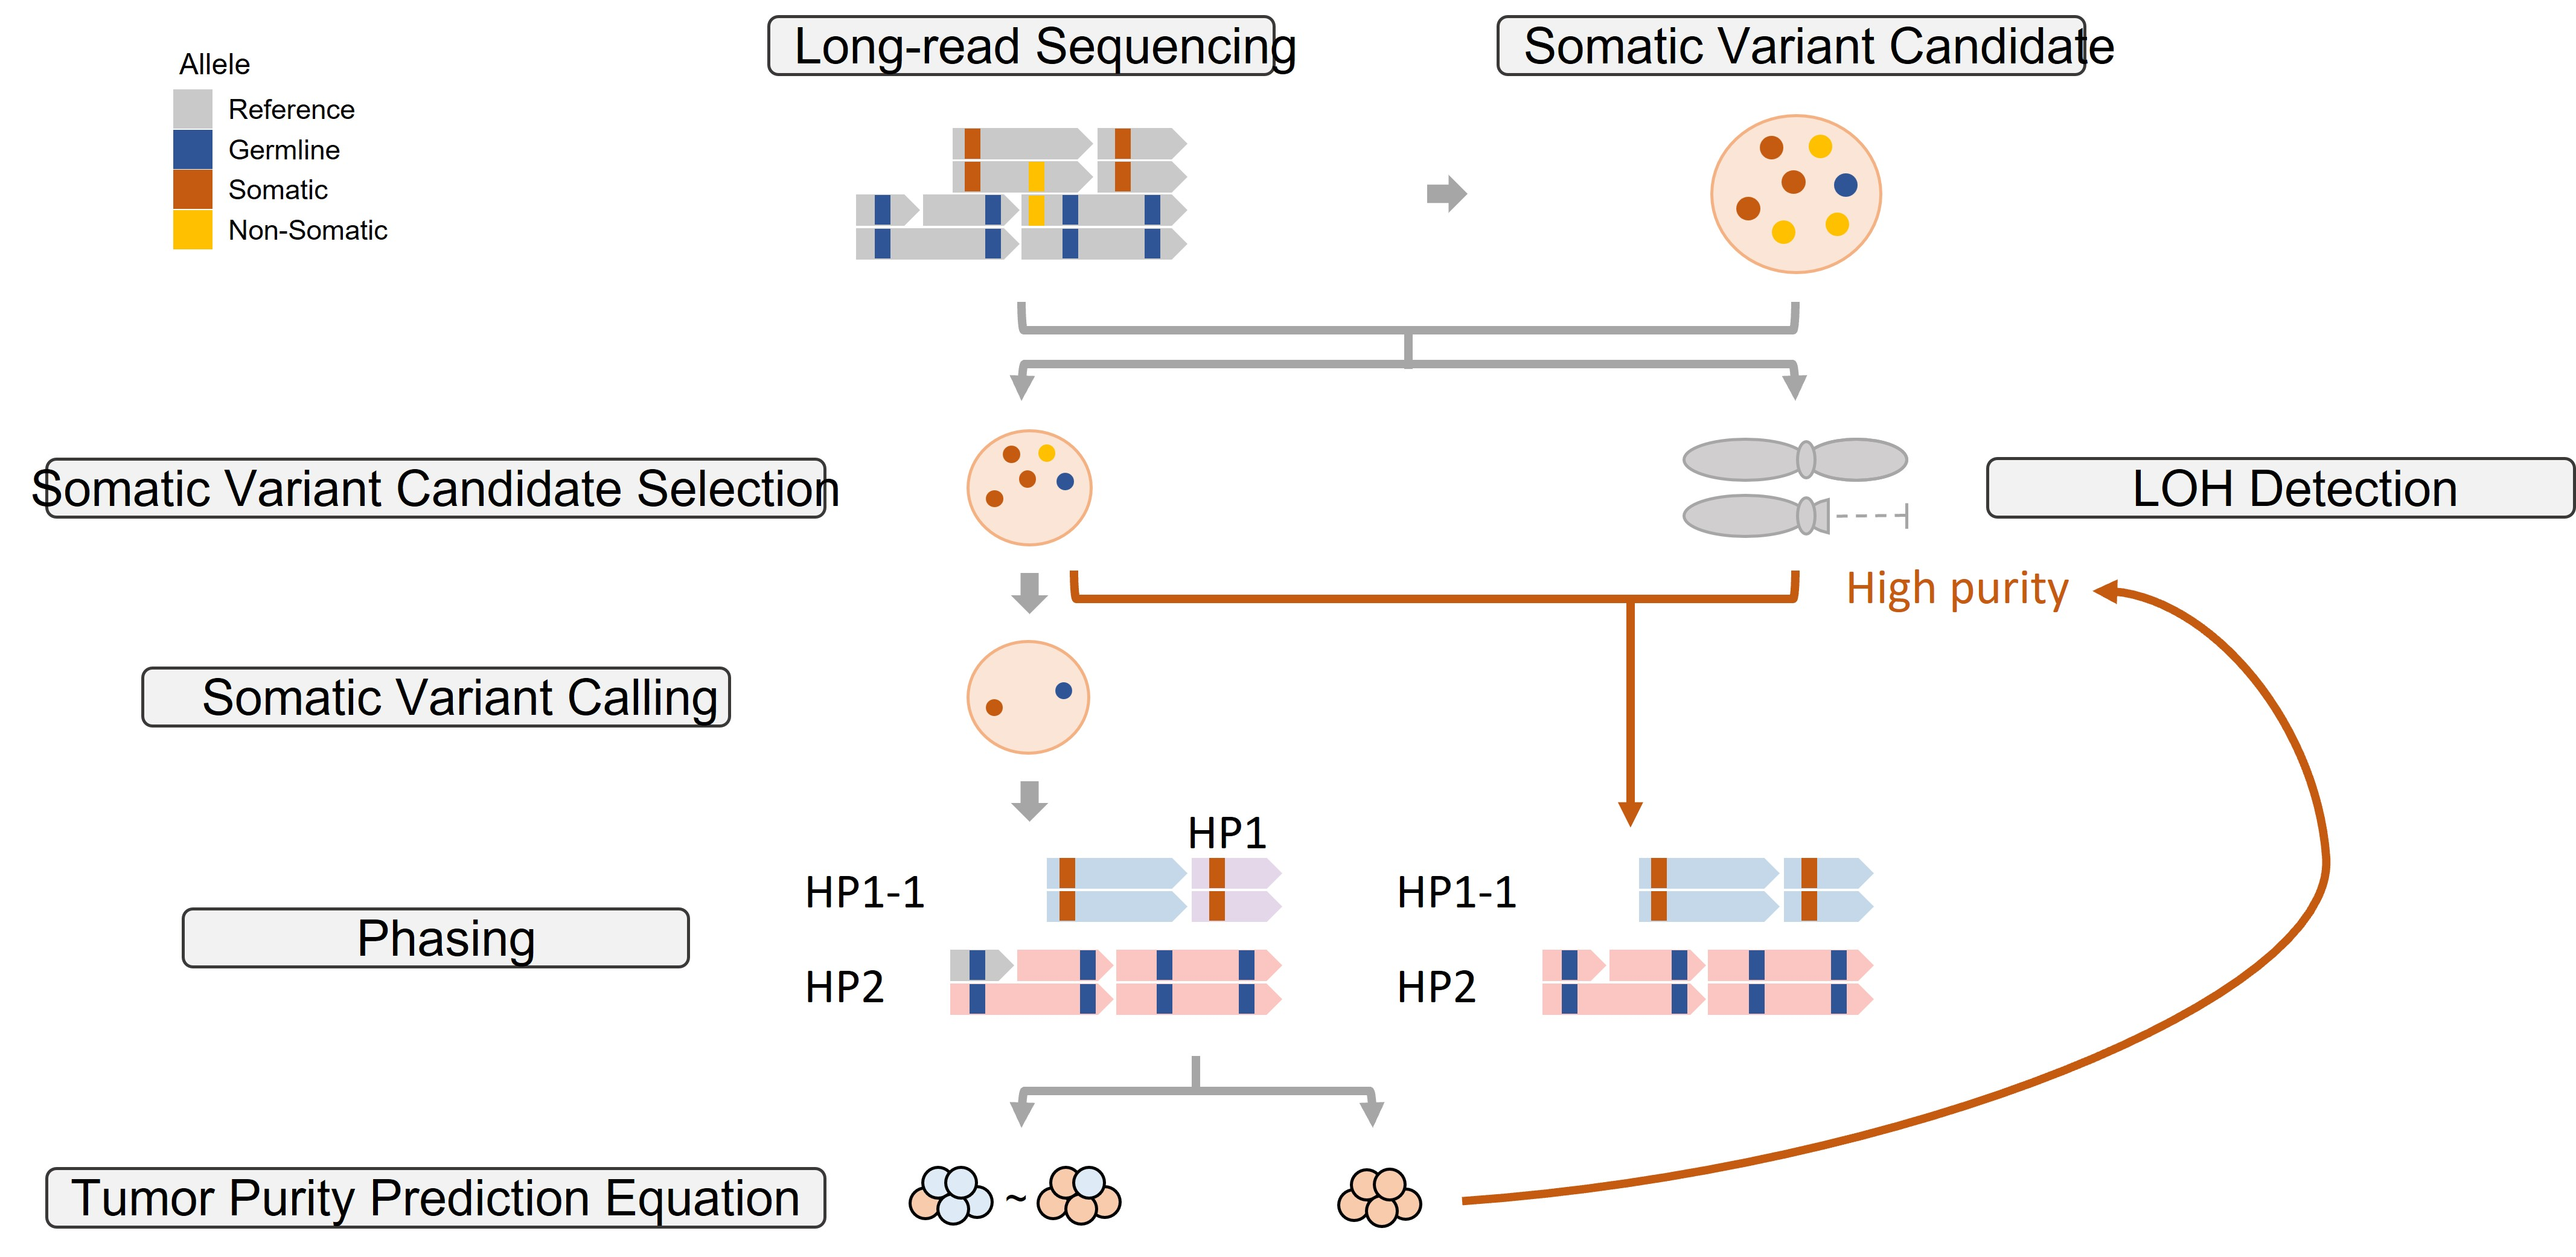
\includegraphics[keepaspectratio]{page_42_cropped.jpg}}
\caption[Integrated Computational Workflow]{Purity-aware computational workflow for somatic variant analysis. For moderate- to low-purity samples, somatic variant calling is applied following candidate selection and phasing. For high-purity samples, where somatic and germline VAFs are indistinguishable, the standard somatic calling step is bypassed to avoid recall loss. Instead, loss-of-heterozygosity (LOH) detection results are iteratively integrated to refine haplotype phasing and preserve analytical accuracy.}\label{fig:app-page-42-cropped-jpg}
\end{figure}

\bibliographystyle{sn-nature}
\nocite{*}
\bibliography{references}

\end{document} 